% Auto-generated by scripts/07b_build_counterfactuals_appendix.R.
\clearpage
\section{Counterfactuals}
\label{sec:app-counterfactuals}

This appendix reports the country-level policy inventory, sensitivity to alternative counterfactual
constructions, the product-group decomposition of annual policy effects, and country-level observed
and counterfactual headline inflation series. Each country figure combines all simulated energy and
food price-policy layers using the HICP item weights in the national CPI basket.

\subsection{Policy Inventory and Counterfactual Definitions}
\label{sec:app-counterfactual-definitions}

Tables~\ref{tab:ea20-price-counterfactual-measures} and~\ref{tab:tariff-shield-formula-comparison} separate the coverage of the policy inventory from the rules used to construct counterfactual prices.

\begin{landscape}
% Auto-generated from data/counterfactual_measure_assumptions.xlsx (include = TRUE).
\fontsize{8.5}{9.4}\selectfont
\setlength{\LTleft}{0pt}
\setlength{\LTright}{0pt}
\setlength{\tabcolsep}{2pt}
\renewcommand{\arraystretch}{1.12}
\captionsetup{hypcap=false}
\captionof{table}{Price measures included in the national counterfactual estimates}
\label{tab:ea20-price-counterfactual-measures}
\vspace{0.3em}
\begin{longtable}{@{}p{0.75in}p{4.0in}p{0.85in}p{1.75in}p{1.4in}@{}}
\toprule
Country & Simplified policy coverage & Policy years & Effect identification & Policy count \\
\midrule
\endfirsthead
\toprule
Country & Simplified policy coverage & Policy years & Effect identification & Policy count \\
\midrule
\endhead
\midrule
\multicolumn{5}{r}{\emph{Continued on next page}}\\
\endfoot
\bottomrule
\endlastfoot
Austria & Products: electricity, gas. Instruments: price caps or regulated tariffs, tax and charge relief, subsidies or rebates. & 2022--2024 & 1 source-determined; 3 model-imputed (official formula, representative bill input). & 4 entries; 3 distinct policies \\
Belgium & Products: electricity, gas, motor fuels. Instruments: price caps or regulated tariffs, tax and charge relief, subsidies or rebates. & 2022--2023 & 2 source-determined; 4 model-imputed. & 6 entries; 3 distinct policies \\
Croatia & Products: food, electricity, gas, heating. Instruments: price caps or regulated tariffs, tax and charge relief, subsidies or rebates. & 2022--2023 & 7 source-determined; 2 model-imputed. & 9 entries; 4 distinct policies \\
Cyprus & Products: electricity, heating, motor fuels. Instruments: price caps or regulated tariffs, tax and charge relief, subsidies or rebates. & 2021--2023 & 1 source-determined; 4 model-imputed. & 5 entries; 3 distinct policies \\
Estonia & Products: electricity, gas, heating, motor fuels. Instruments: price caps or regulated tariffs, tax and charge relief, subsidies or rebates. & 2021--2024 & 0 source-determined; 8 model-imputed. & 8 entries; 8 distinct policies \\
Finland & Products: electricity, motor fuels, passenger transport. Instruments: tax and charge relief. & 2022--2023 & 5 source-determined; 1 model-imputed. & 6 entries; 3 distinct policies \\
France & Products: electricity, gas, motor fuels. Instruments: price caps or regulated tariffs, subsidies or rebates. & 2021--2024 & 2 source-determined; 1 model-imputed. & 3 entries; 3 distinct policies \\
Germany & Products: electricity, gas, heating, motor fuels. Instruments: price caps or regulated tariffs, tax and charge relief, subsidies or rebates. & 2022--2024 & 1 source-determined; 6 model-imputed. & 7 entries; 6 distinct policies \\
Greece & Products: electricity, gas, motor fuels. Instruments: subsidies or rebates. & 2021--2023 & 0 source-determined; 3 model-imputed. & 3 entries; 3 distinct policies \\
Ireland & Products: electricity, gas, motor fuels. Instruments: tax and charge relief, subsidies or rebates. & 2022--2023 & 2 source-determined; 5 model-imputed. & 7 entries; 7 distinct policies \\
\pagebreak
Italy & Products: electricity, gas, motor fuels. Instruments: tax and charge relief, subsidies or rebates. & 2021--2023 & 3 source-determined; 5 model-imputed. & 8 entries; 5 distinct policies \\
Latvia & Products: electricity, gas, heating. Instruments: price caps or regulated tariffs, tax and charge relief, subsidies or rebates. & 2022--2023 & 0 source-determined; 3 model-imputed. & 3 entries; 3 distinct policies \\
Lithuania & Products: electricity, gas. Instruments: subsidies or rebates. & 2022--2023 & 0 source-determined; 2 model-imputed. & 2 entries; 1 distinct policy \\
Luxembourg & Products: electricity, gas, heating, motor fuels, other consumption. Instruments: price caps or regulated tariffs, tax and charge relief, subsidies or rebates. & 2022--2024 & 67 source-determined; 5 model-imputed. & 72 entries; 6 distinct policies \\
Malta & Products: electricity, motor fuels. Instruments: price caps or regulated tariffs, subsidies or rebates. & 2022--2023 & 0 source-determined; 2 model-imputed. & 2 entries; 2 distinct policies \\
Netherlands & Products: electricity, gas, heating, motor fuels. Instruments: price caps or regulated tariffs, tax and charge relief. & 2022--2023 & 7 source-determined; 4 model-imputed. & 11 entries; 6 distinct policies \\
Portugal & Products: food, electricity, gas, motor fuels. Instruments: price caps or regulated tariffs, tax and charge relief. & 2021--2026 & 1 source-determined; 14 model-imputed. & 15 entries; 8 distinct policies \\
Slovakia & Products: electricity, gas, heating. Instruments: price caps or regulated tariffs, tax and charge relief. & 2023 & 0 source-determined; 3 model-imputed. & 3 entries; 1 distinct policy \\
Slovenia & Products: electricity, gas, heating, motor fuels. Instruments: price caps or regulated tariffs, tax and charge relief. & 2021--2023 & 0 source-determined; 9 model-imputed. & 9 entries; 7 distinct policies \\
Spain & Products: food, electricity, gas, motor fuels. Instruments: price caps or regulated tariffs, tax and charge relief, subsidies or rebates. & 2021--2026 & 5 source-determined; 10 model-imputed. & 15 entries; 9 distinct policies \\
\midrule\textbf{Euro area} & \textbf{Sum of the 20 country rows.} & \textbf{2021--2026} & \textbf{104 source-determined; 94 model-imputed.} & \textbf{198 entries; 91 distinct policies} \\
\end{longtable}
\par\vspace{0.25em}\fontsize{8}{8.8}\selectfont\noindent Notes: Products and instruments are grouped for readability; the underlying workbook retains the measure-level descriptions, dates, COICOP codes, and the measure-specific evidence basis. Source-determined effects are quantified directly from statutory tax rates, regulated tariffs, or official administrative price or bill series. Model-imputed effects require an aggregate-equivalent wedge, representative bill, calibrated pass-through, or model-based proxy. An official policy announcement alone does not make an effect source-determined when its price effect must be estimated. Policy count reports executed country-product entries and distinct policy devices. The distinct count consolidates successive phases or extensions and a single legal measure represented by several product trajectories; for example, Luxembourg's product-specific VAT trajectories count as one policy. The Euro-area row is the sum of the 20 country rows. Sources: Bruegel Dataset (2021), `National policies to shield consumers from rising energy prices,' version of 26 June 2023; authors' calculations.

\end{landscape}
% The inventory uses both captionof and longtable; undo longtable's second counter step.
\addtocounter{table}{-1}
\clearpage

\noindent\begin{minipage}{\linewidth}
\centering
\fontsize{7.6}{8.5}\selectfont
\setlength{\tabcolsep}{3.5pt}
\renewcommand{\arraystretch}{1.10}
\captionof{table}{Official energy-price-support rules and their counterfactual implementation}
\label{tab:tariff-shield-formula-comparison}
\begin{tabularx}{\linewidth}{@{}p{1.7cm}p{4.25cm}Xp{4.0cm}@{}}
\toprule
Country and policy & Official rule & Implementation & Main difference \tabularnewline
\midrule
Austria: electricity price brake
& $S=\min(Q,2{,}900)\min\{\max(p-0.10,0),0.30\}$; $B^{1}=B^{0}-S$.
& E-Control bill: $Q=3{,}500$, $p=\text{EUR }0.24$/kWh; official non-energy
components and VAT. $\widehat{\rho}=B^{0}/B^{1}=1.433$.
& Statutory rule on a representative bill; no contract-price, consumption, or billing-date distribution. \tabularnewline
\addlinespace
Germany: electricity and gas price brakes
& Relief: $S=\alpha Q^{0}\max(p-c,0)$; bill: $B^{1}=F+pQ-S$.
$\alpha=0.8$; caps: EUR 0.40/kWh (electricity), EUR 0.12/kWh (gas).
& Same bill rule; representative contract. $p$: BNetzA April 2023 price,
monthly HICP path. Baseline: $Q/Q^{0}=1$, $F=0$;
$\widehat{\rho}=B^{0}/B^{1}$.
& Contract-level rule versus representative contract; no distribution of
prices, fixed charges, or consumption. \tabularnewline
\addlinespace
Netherlands: 2023 electricity and gas price cap
& Relief: $S=\min(Q,\bar Q)\max(p-c,0)$. Caps: EUR 0.40/kWh up to 2,900 kWh;
EUR 1.45/m$^{3}$ up to 1,200 m$^{3}$.
& CBS monthly contract and capped tariffs. $B^{0}=B^{1}+Q(p-p^{\mathrm{cap}})$;
$\widehat{\rho}=B^{0}/B^{1}$. Representative quantities: 2,063 kWh and 1,136 m$^{3}$.
& Average bills and quantities versus household billing dates, consumption,
and contract tariffs. \tabularnewline
\addlinespace
Italy: electricity and gas social bonuses
& Bill credit: $S_{iq}(d)=CCI_{iq}d/D_q$, plus ordinary bonus. $CCI_{iq}$:
quarter- and beneficiary-specific.
& ARERA aggregate funding:
$\widehat{\rho}_{jq}=E^{0}_{jq}/(E^{0}_{jq}-S_{jq})$;
$E^{0}_{jq}$: domestic volume $\times$ average final price.
& Means-tested bill credit versus aggregate HICP wedge; no eligibility,
family-size, heating-use, or take-up incidence. \tabularnewline
\addlinespace
Spain: Iberian electricity-market adjustment
& Generator adjustment: $Y_d=\max\{(P^{\mathrm{gas}}_d-P^{\mathrm{ref}}_d)/0.55,0\}$
per MWh; cost allocated to non-exempt demand.
& OMIE hourly settlements: $P^{1}_h=P^{\mathrm{OMIE}}_h+A^{C}_h$;
$P^{0}_h=P^{\mathrm{OMIE}}_h+A^{P}_h$; $\rho_h=P^{0}_h/P^{1}_h$.
& Published wholesale wedge; no recomputation of $Y_d$ or retail exemptions;
proportional HICP transmission. \tabularnewline
\addlinespace
France: gas and electricity tariff shields
& No reconstructed formula: CRE and Insee publish observed and no-shield
regulated-tariff paths.
& Published tariff-path ratio applied to HICP; documented Insee pass-through
parameters where required.
& Public counterfactual tariff; only HICP mapping requires chaining and
pass-through assumptions. \tabularnewline
\bottomrule
\end{tabularx}
\begin{flushleft}
\fontsize{7.0}{7.9}\selectfont Notes: $F$: fixed charge; $p$: contract price;
$Q$: current consumption; $Q^{0}$: reference consumption; $c$: statutory cap;
$A^{C}$ and $A^{P}$: OMIE consumer and producer adjustments. $\widehat{\rho}$ denotes a
counterfactual-to-observed ratio reconstructed from representative or aggregate inputs; $\rho_h$
is the corresponding directly observed hourly ratio. The table contrasts
official rules with the HICP counterfactual transformation. Sources: Austrian Parliament and
E-Control; Bundesnetzagentur and BMWK; Dutch Government and CBS; ARERA; Spain's Royal Decree-law 10/2022 and
OMIE; CRE and Insee; authors' calculations.
\end{flushleft}
\end{minipage}

\clearpage

\subsection{Sensitivity to Counterfactual Construction}
\label{sec:app-counterfactual-sensitivity}

Table~\ref{tab:ea20-policy-method-sensitivity} compares the full specification with direct
reconstructions only, the exclusion of conditional benchmarks, and alternative benchmark wedges.

\begin{table}[H]
\small
\setlength{\tabcolsep}{4pt}

\caption{\label{tab:ea20-policy-method-sensitivity}Sensitivity of euro-area inflation-inequality effects to counterfactual construction methods}
\centering
\resizebox{\textwidth}{!}{%
\begin{tabular}[t]{lrrrrrr}
\toprule
\multicolumn{1}{c}{} & \multicolumn{6}{c}{Inflation inequality}\\
\cmidrule(lr){2-7}
\multicolumn{1}{c}{} & \multicolumn{3}{c}{Individual P20--P80} & \multicolumn{3}{c}{Income Q1--Q5}\\
\cmidrule(lr){2-4} \cmidrule(lr){5-7}
Scenario & 2021 & 2022 & 2023 & 2021 & 2022 & 2023\\
\midrule
Full specification & -0.1 & -1.8 & -0.7 & -0.1 & -0.6 & -0.6\\
Direct reconstructions only & 0.0 & -1.1 & -0.2 & 0.0 & -0.4 & -0.1\\
Full specification without conditional benchmarks & -0.1 & -1.7 & -0.4 & -0.1 & -0.6 & -0.3\\
Conditional benchmark wedges at 50\% & -0.1 & -1.7 & -0.5 & -0.1 & -0.6 & -0.4\\
Conditional benchmark wedges at 150\% & -0.1 & -1.8 & -0.9 & -0.1 & -0.7 & -0.7\\
\addlinespace
Dependence on estimated layers: full minus direct-only & -0.1 & -0.7 & -0.4 & 0.0 & -0.3 & -0.4\\
\bottomrule
\end{tabular}
}%
\begin{flushleft}
\footnotesize{Notes. The first block reports the observed minus counterfactual P20--P80 range of annual household inflation, in percentage points. The range is P80 minus P20. National percentile endpoints use HBS survey weights and are averaged with annual HICP country weights over the 19-country household sample; Portugal is excluded. The second block reports the corresponding Q1--Q5 effects for all 20 euro-area countries. Direct reconstructions use statutory rates, unit rebates, or published reference-price paths without a fitted intensity. The 50\% and 150\% rows scale only the conditional benchmark price wedges. Full minus direct-only measures dependence on estimated layers; it is not a confidence interval. Sources: Eurostat, HBS 2020 microdata, national sources, authors' calculations.}
\end{flushleft}
\end{table}

\clearpage

\subsection{Country-Level Observed and Counterfactual Inflation}
\label{sec:app-country-counterfactual-figures}

Figures~\ref{fig:country-counterfactuals-1}--\ref{fig:country-counterfactuals-4} compare observed inflation with the counterfactual that removes household price policies.

\begin{figure}[H]
\centering
\begin{minipage}[t]{0.485\textwidth}\centering
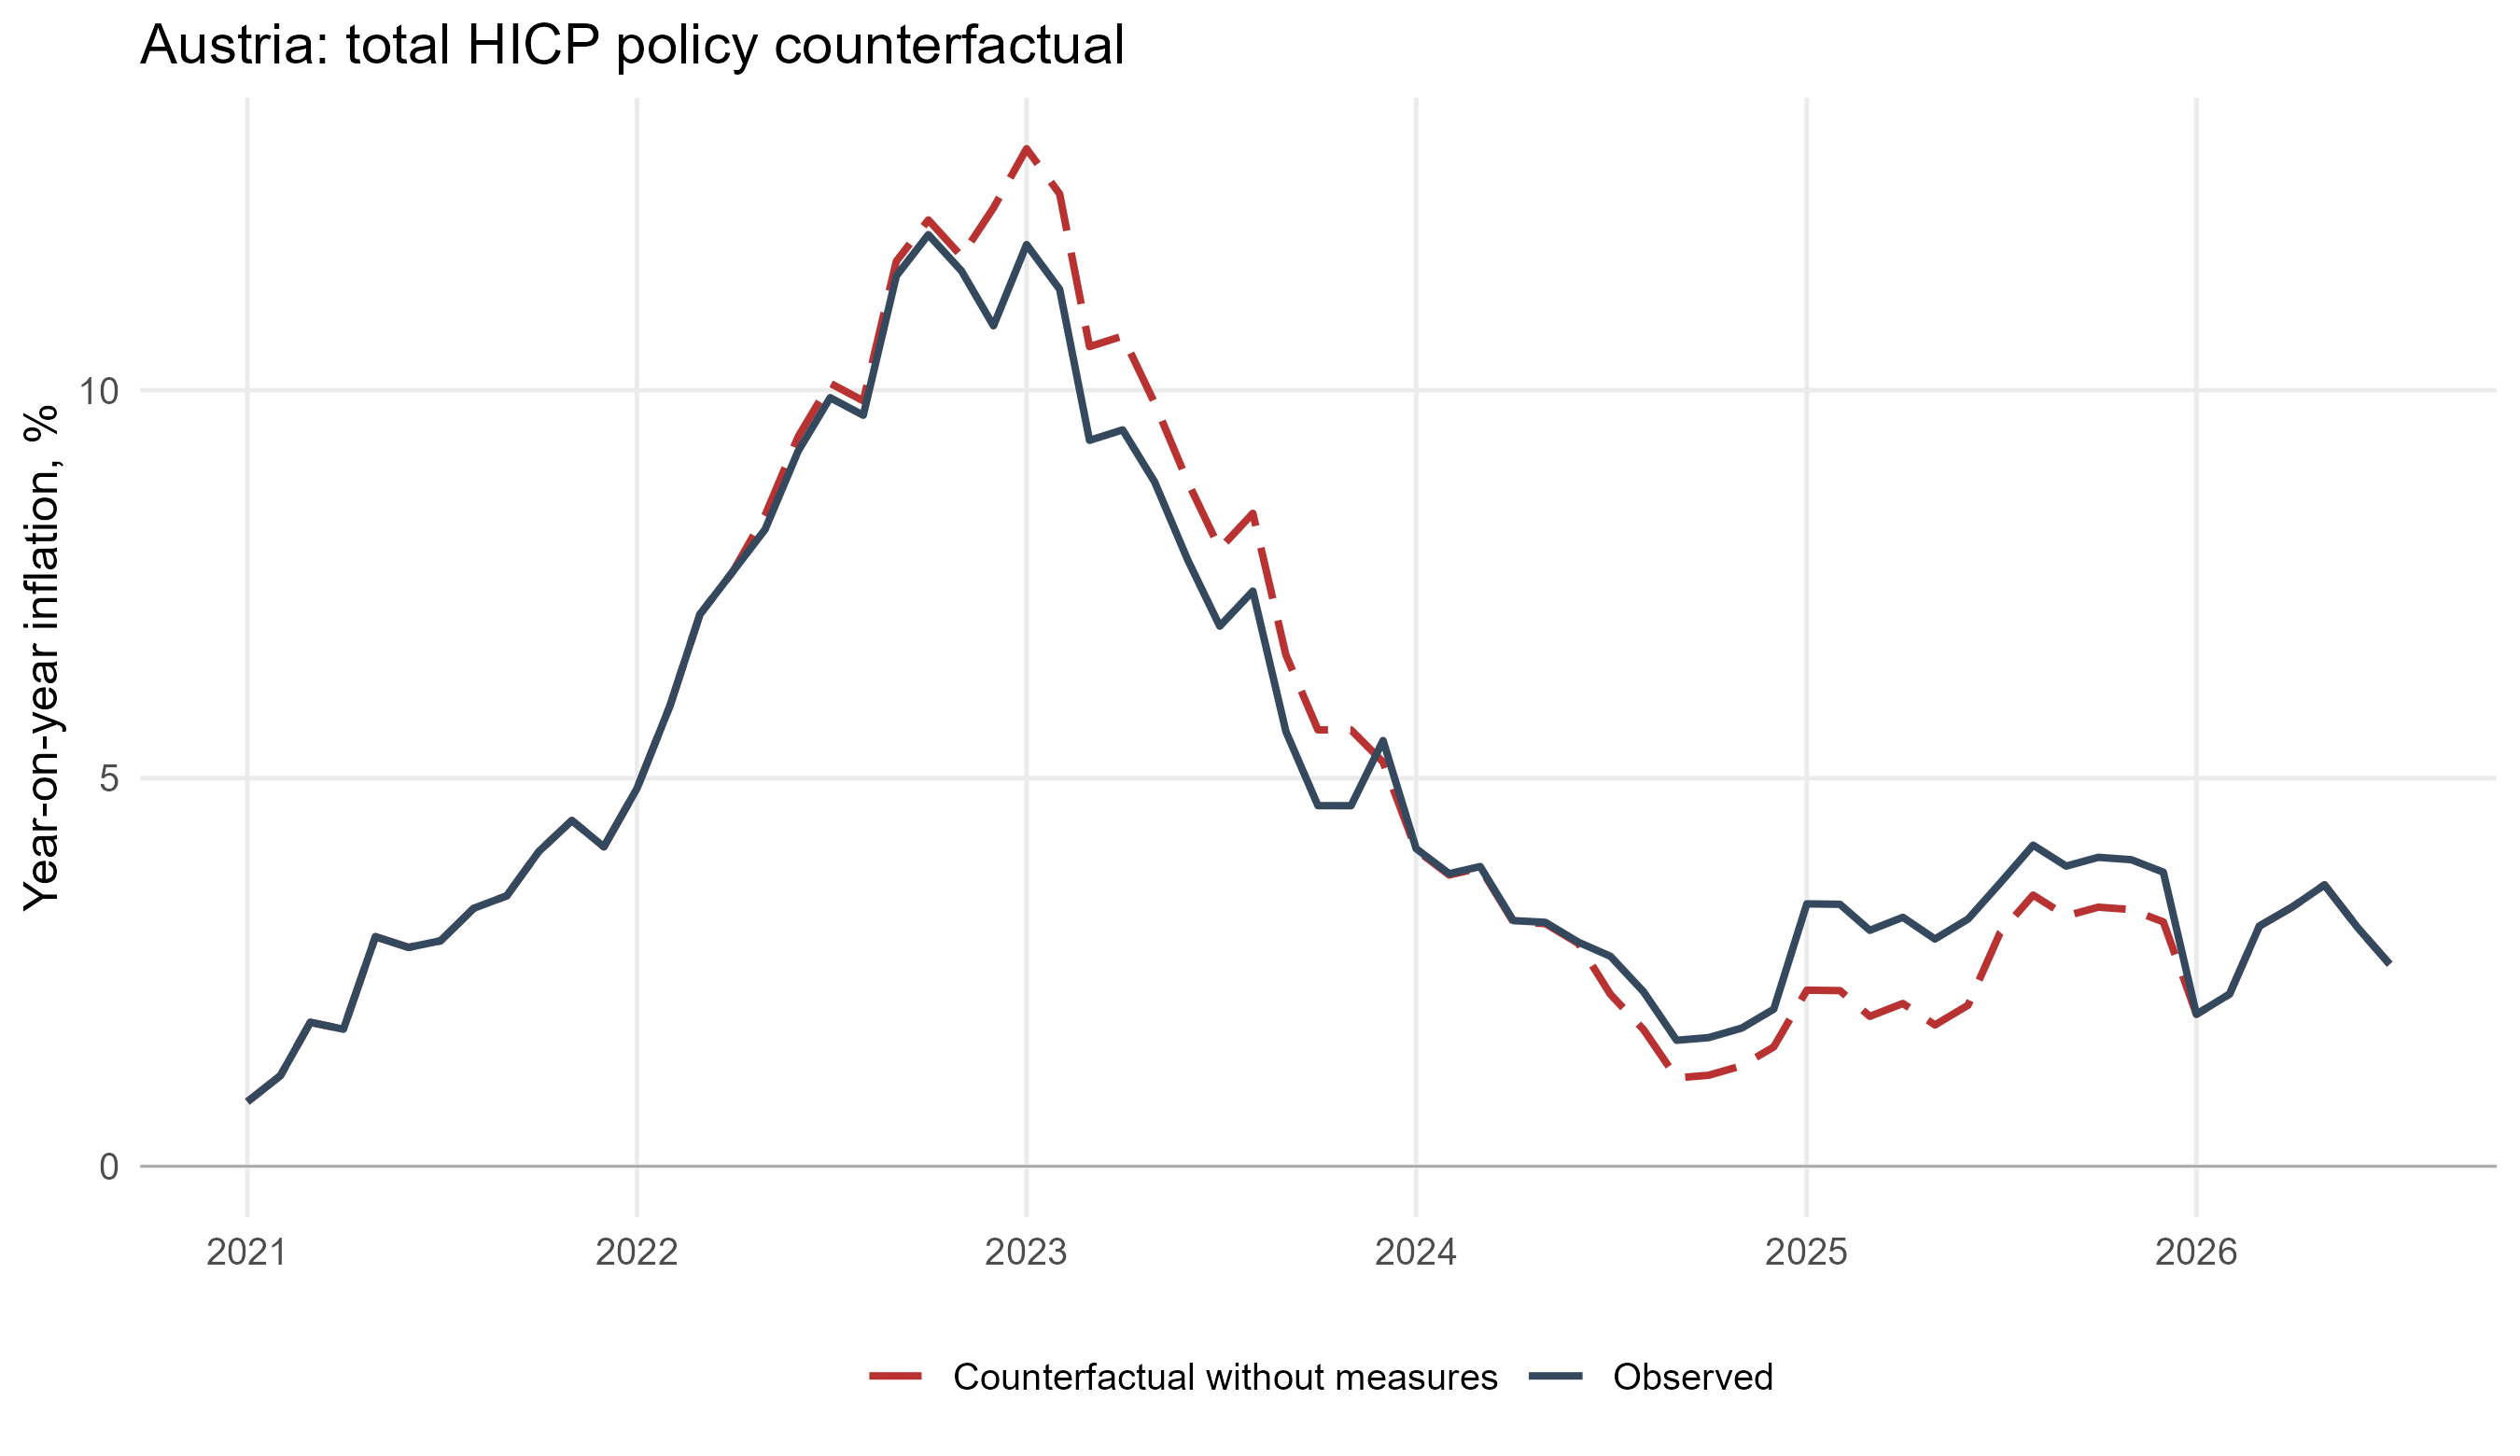
\includegraphics[width=\linewidth,height=0.225\textheight,keepaspectratio]{fig/policy_total_cpi_counterfactual_inflation_AT_austria.png}\\[-0.4em]\textbf{(a) Austria}
\end{minipage}\hfill
\begin{minipage}[t]{0.485\textwidth}\centering
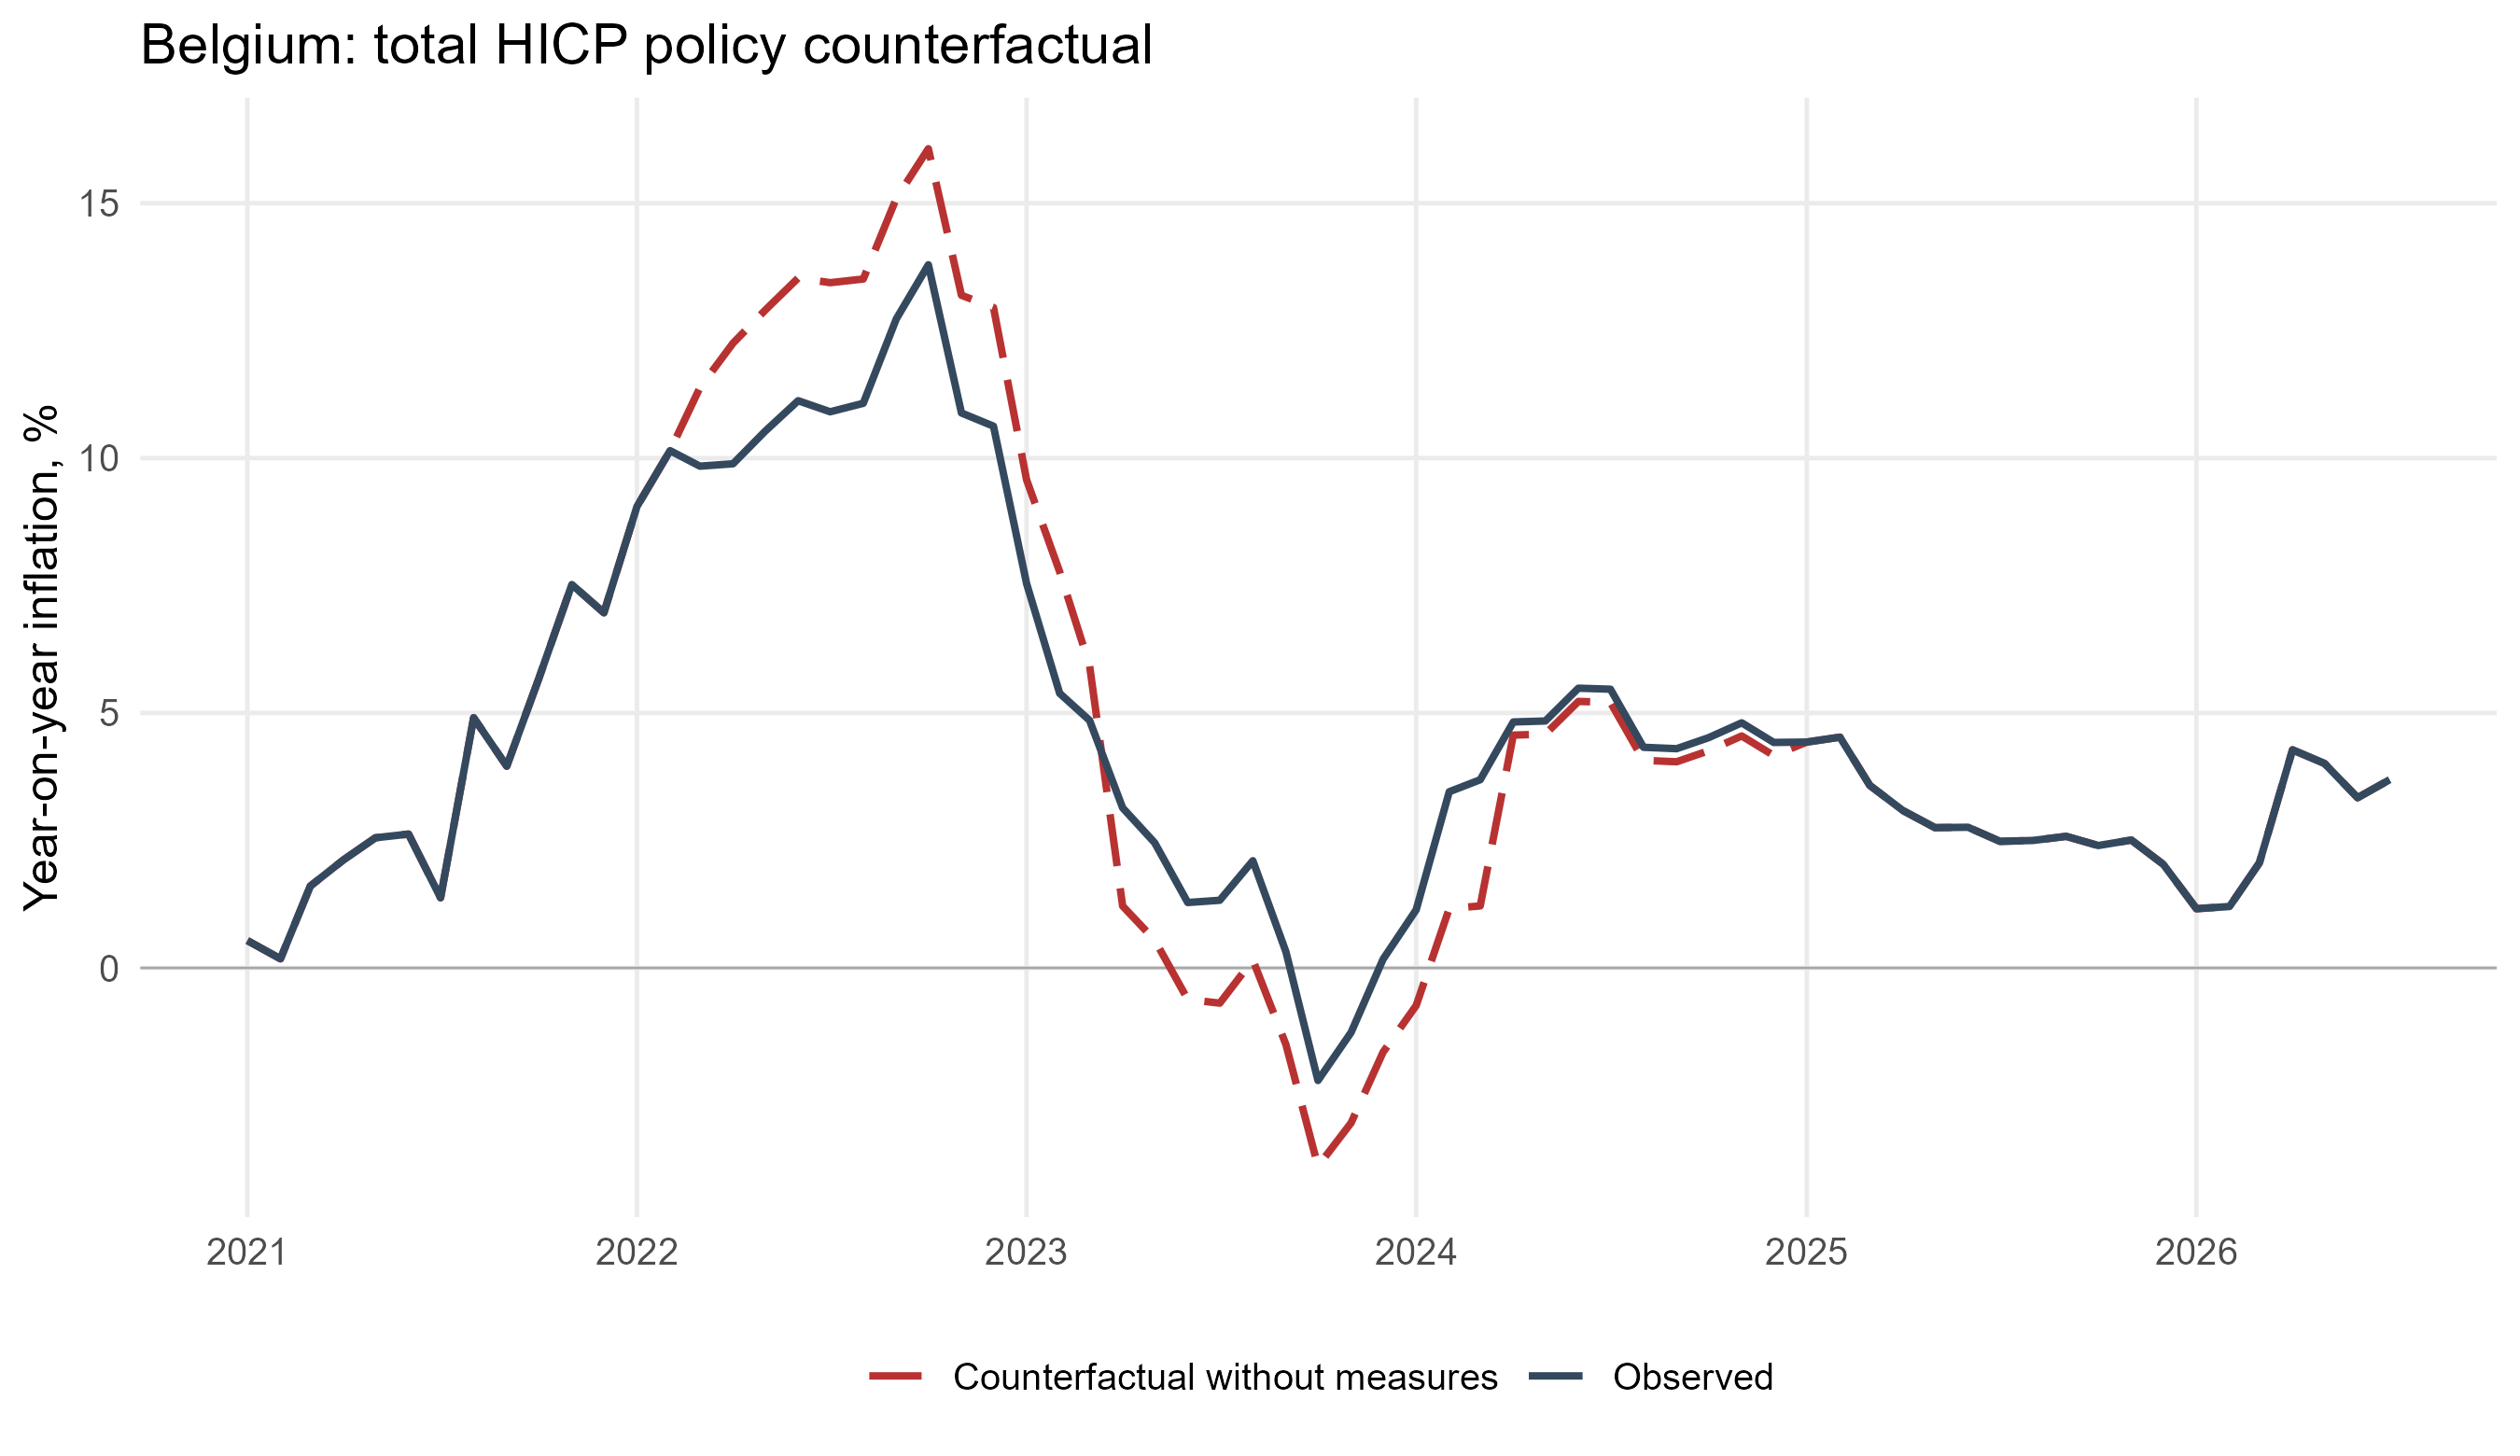
\includegraphics[width=\linewidth,height=0.225\textheight,keepaspectratio]{fig/policy_total_cpi_counterfactual_inflation_BE_belgium.png}\\[-0.4em]\textbf{(b) Belgium}
\end{minipage}

\vspace{0.25em}
\begin{minipage}[t]{0.485\textwidth}\centering
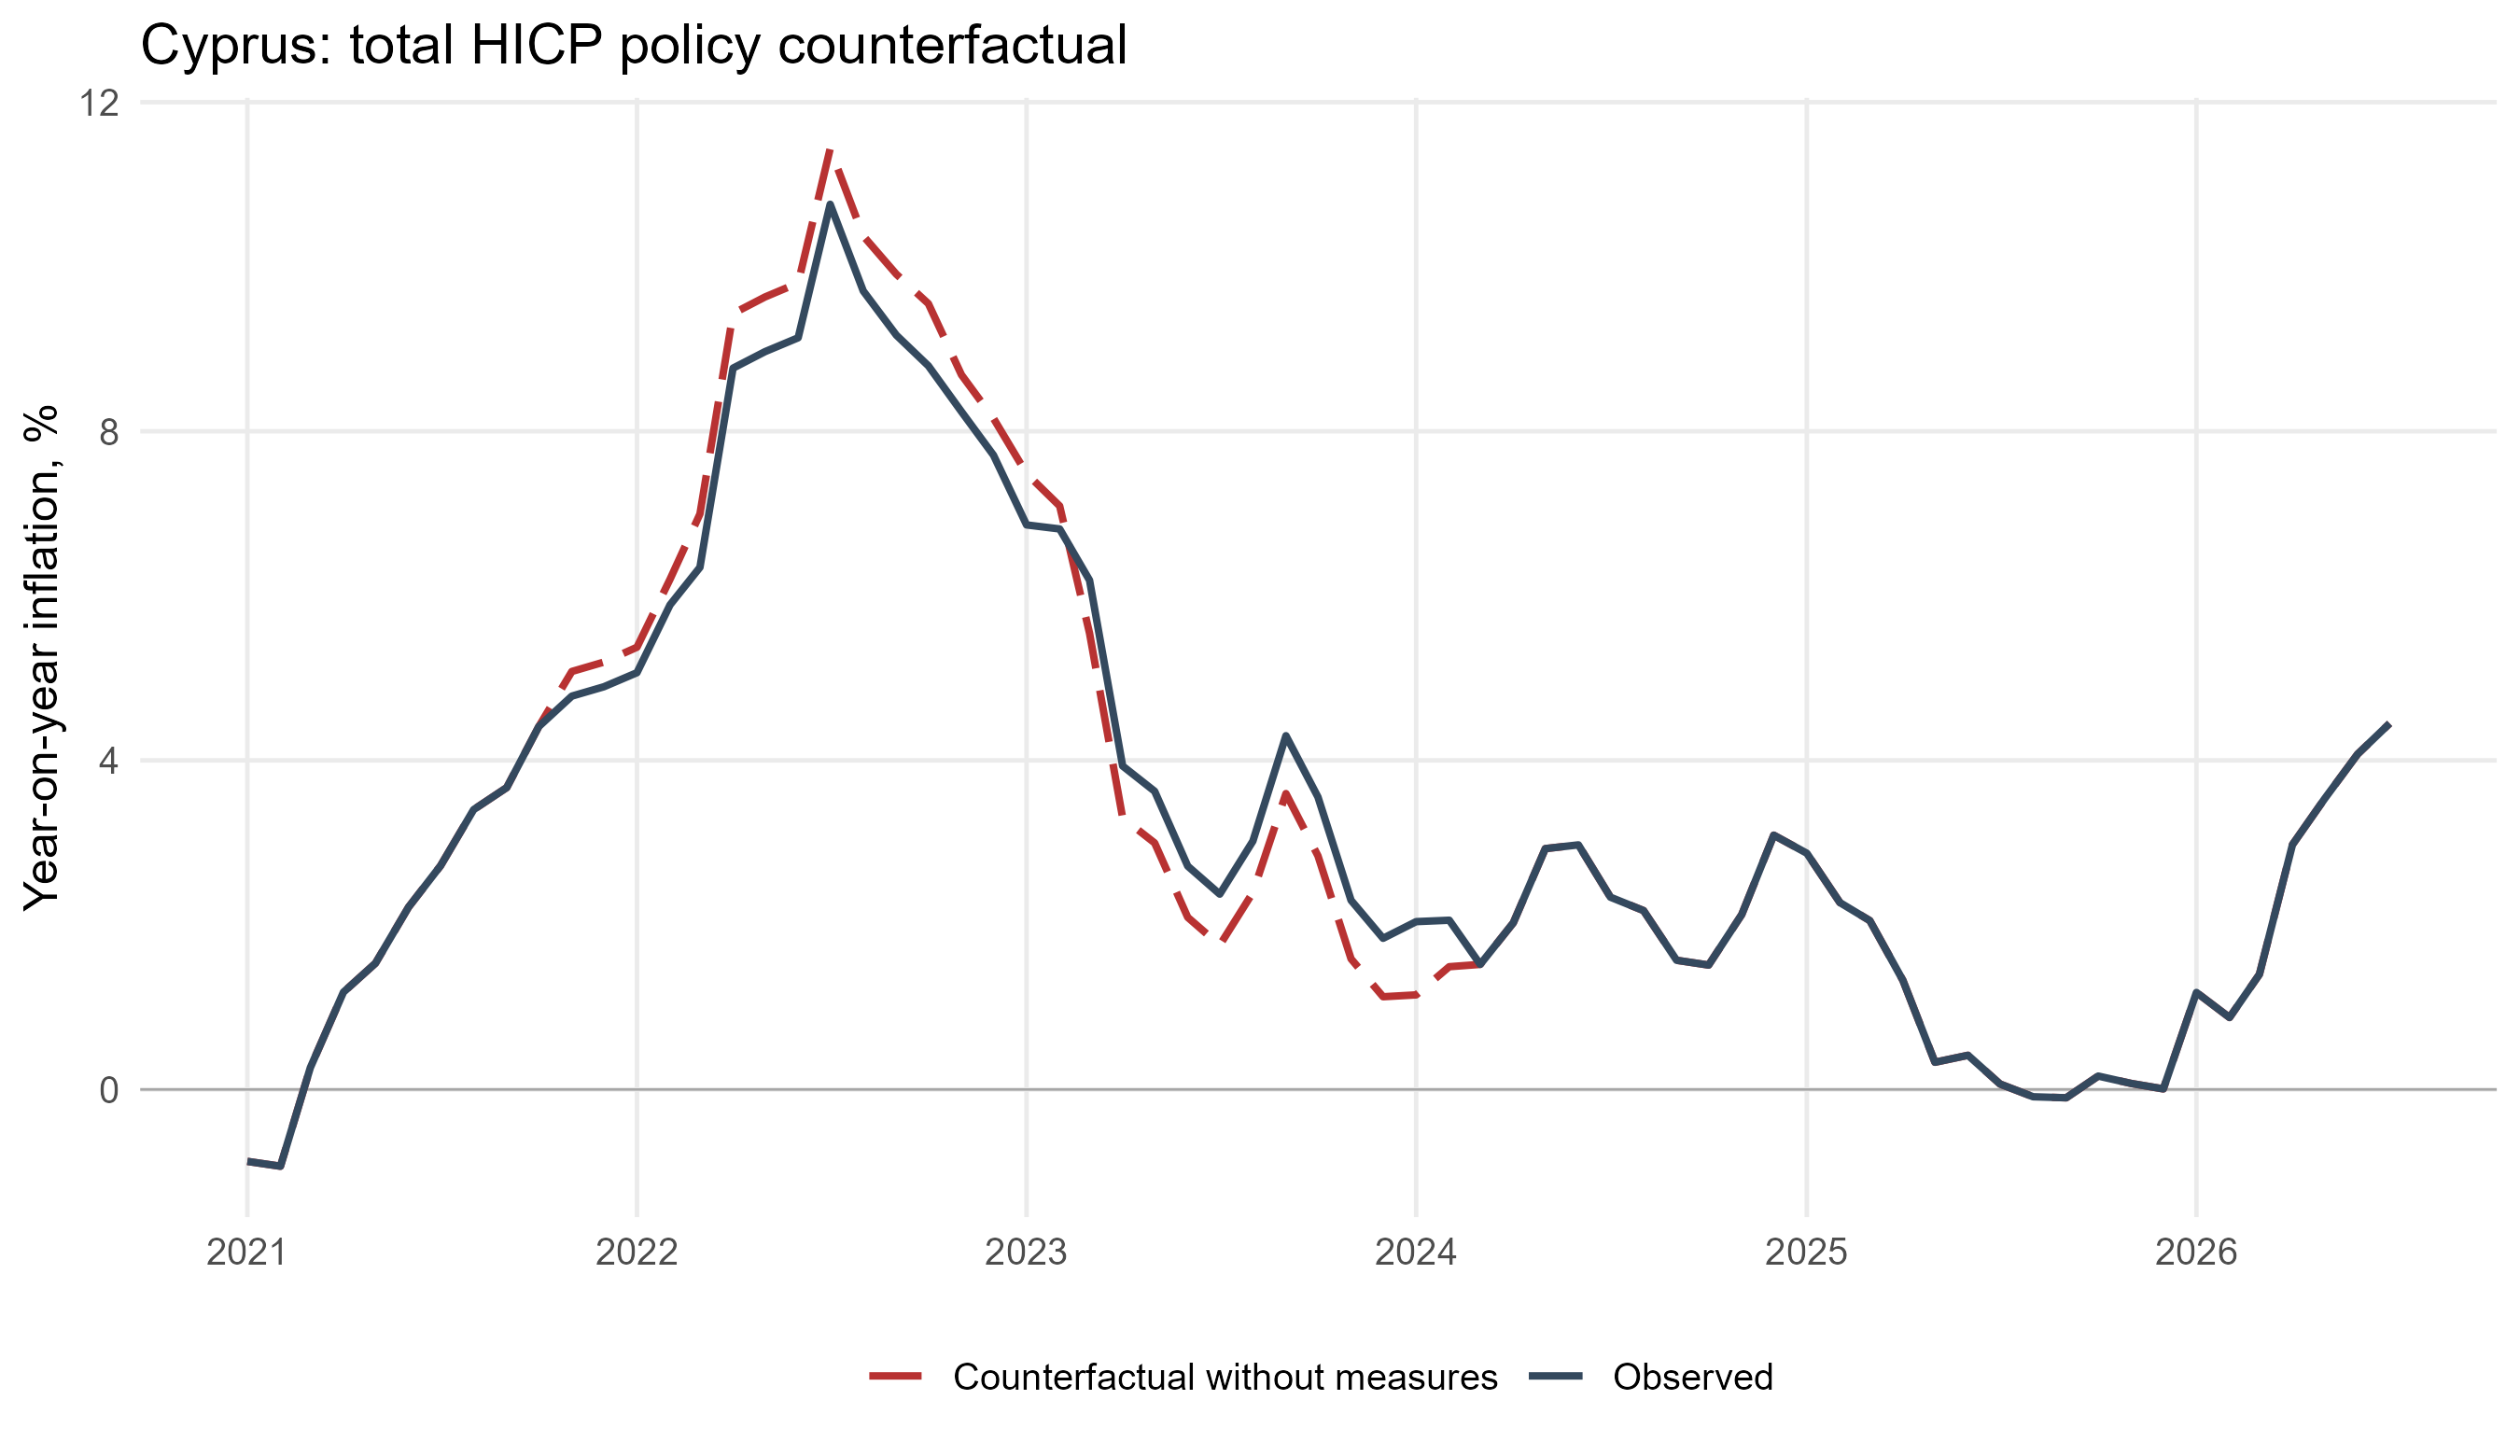
\includegraphics[width=\linewidth,height=0.225\textheight,keepaspectratio]{fig/policy_total_cpi_counterfactual_inflation_CY_cyprus.png}\\[-0.4em]\textbf{(c) Cyprus}
\end{minipage}\hfill
\begin{minipage}[t]{0.485\textwidth}\centering
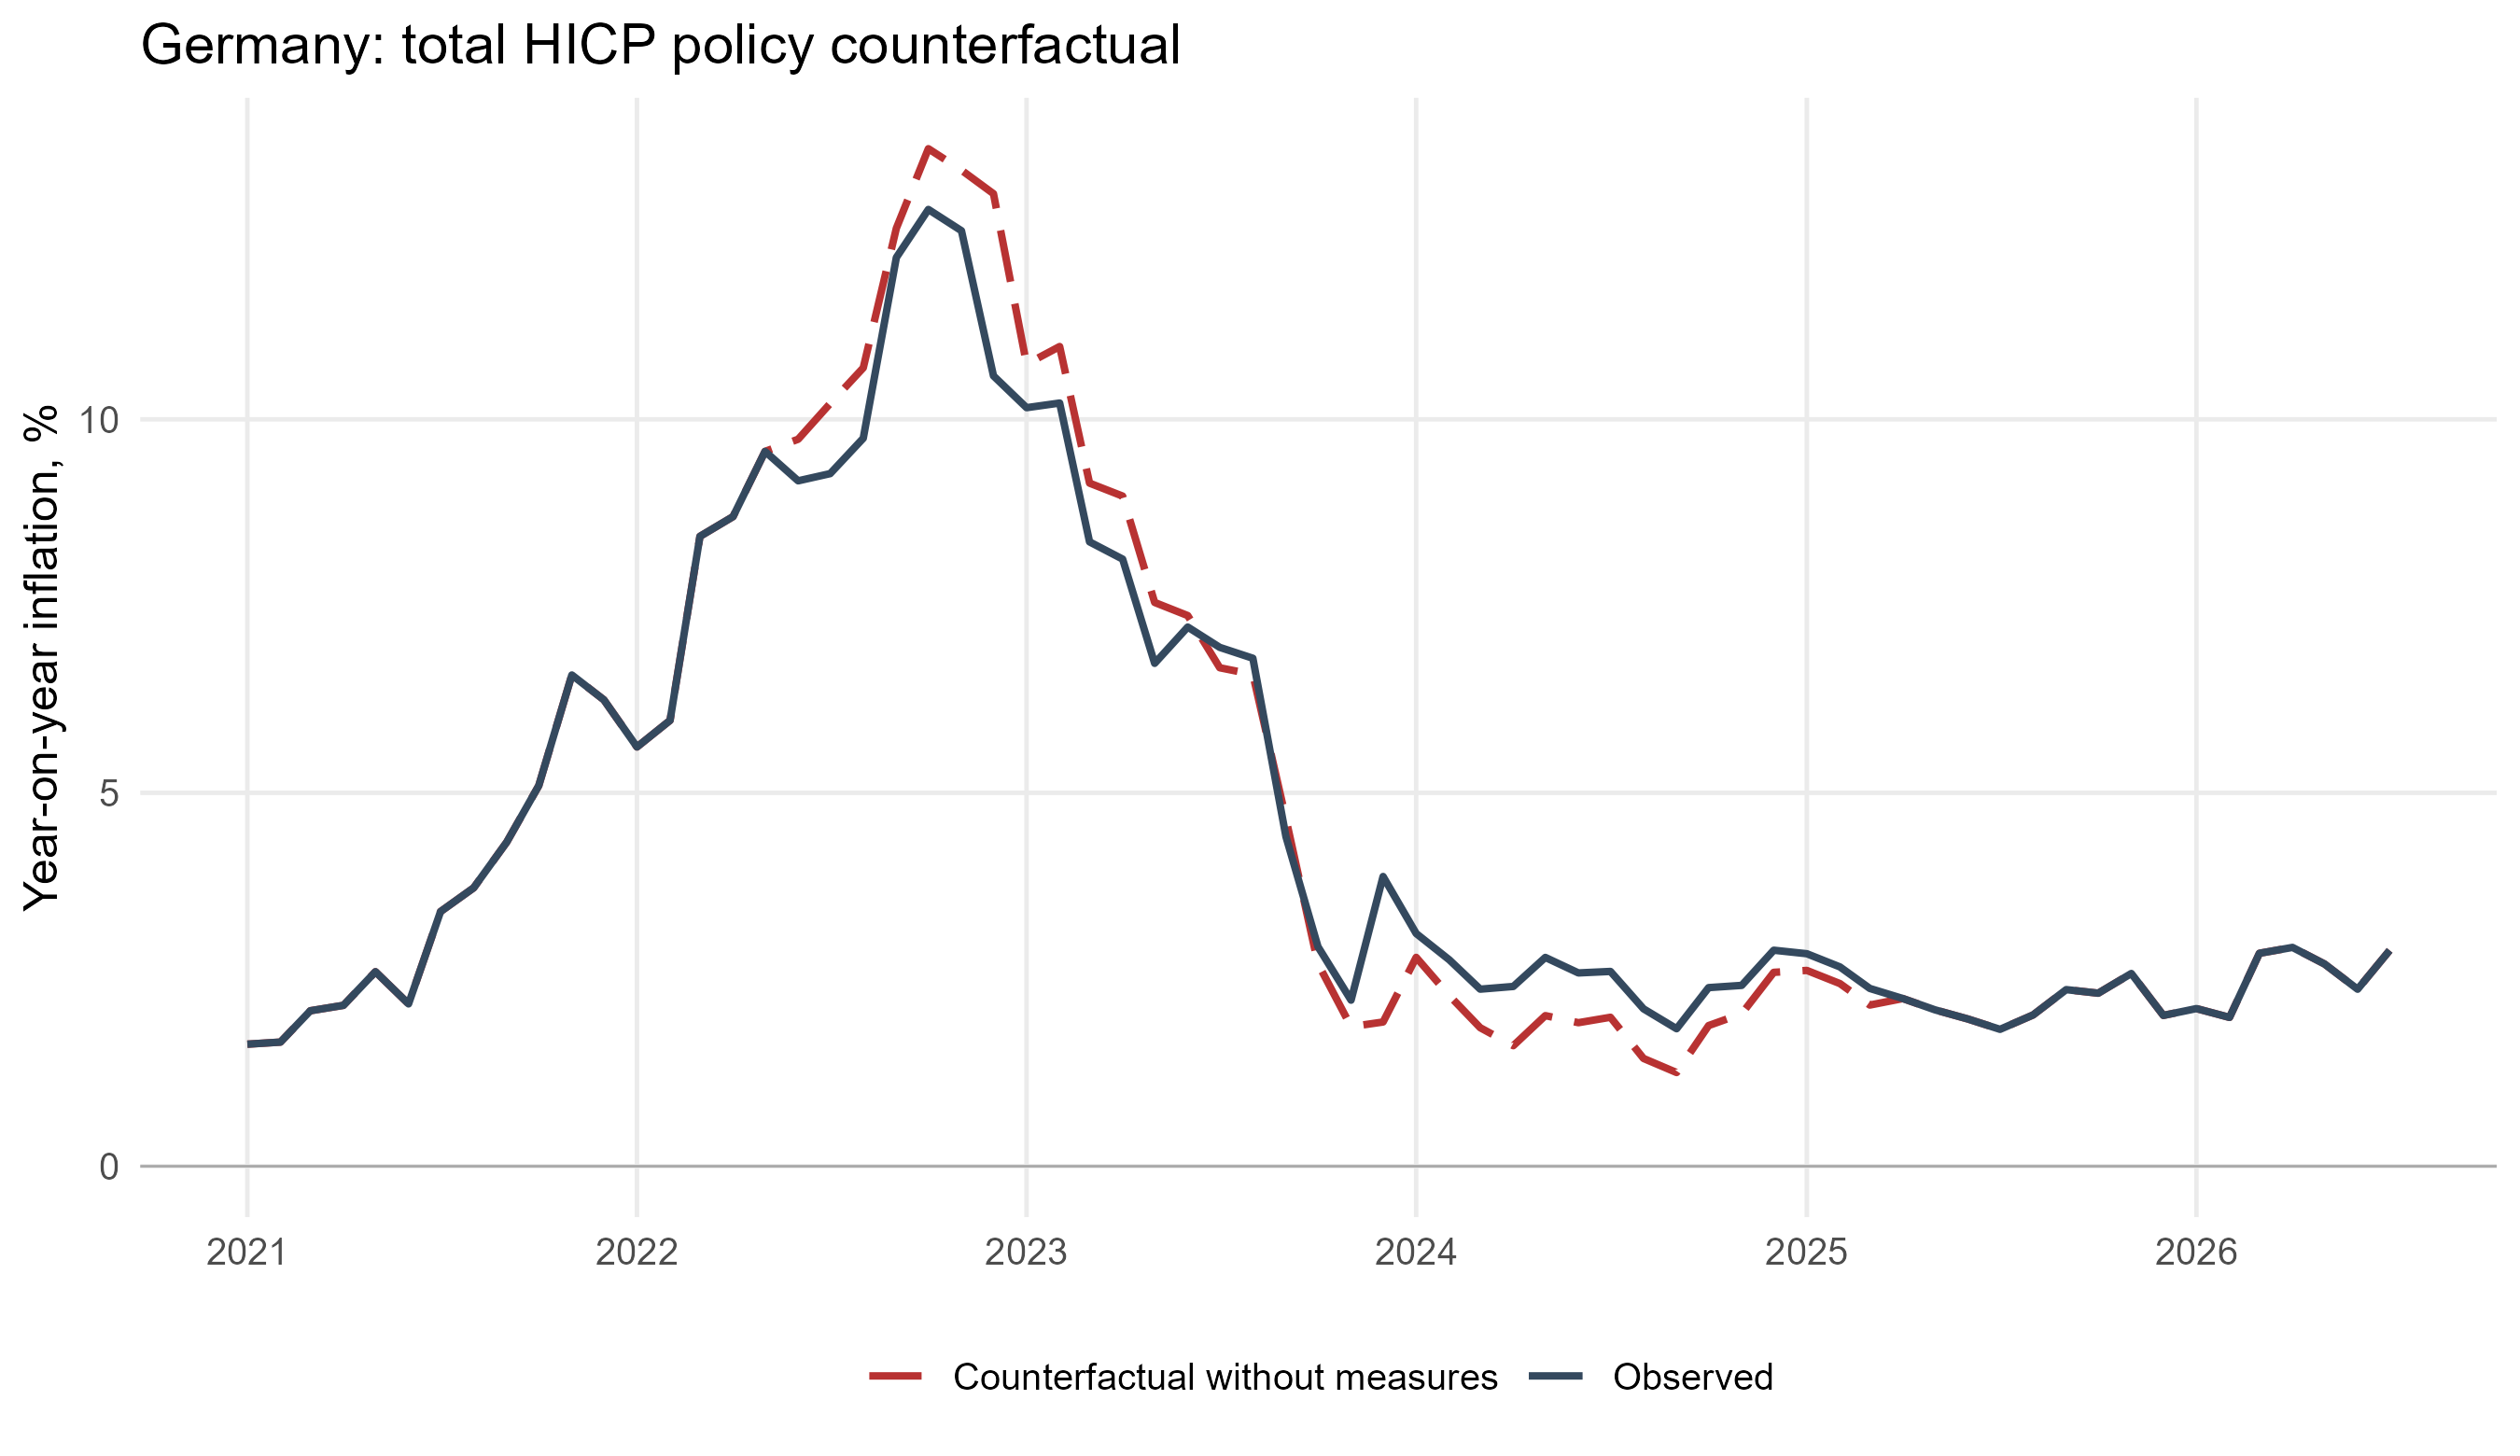
\includegraphics[width=\linewidth,height=0.225\textheight,keepaspectratio]{fig/policy_total_cpi_counterfactual_inflation_DE_germany.png}\\[-0.4em]\textbf{(d) Germany}
\end{minipage}

\vspace{0.25em}
\begin{minipage}[t]{0.485\textwidth}\centering
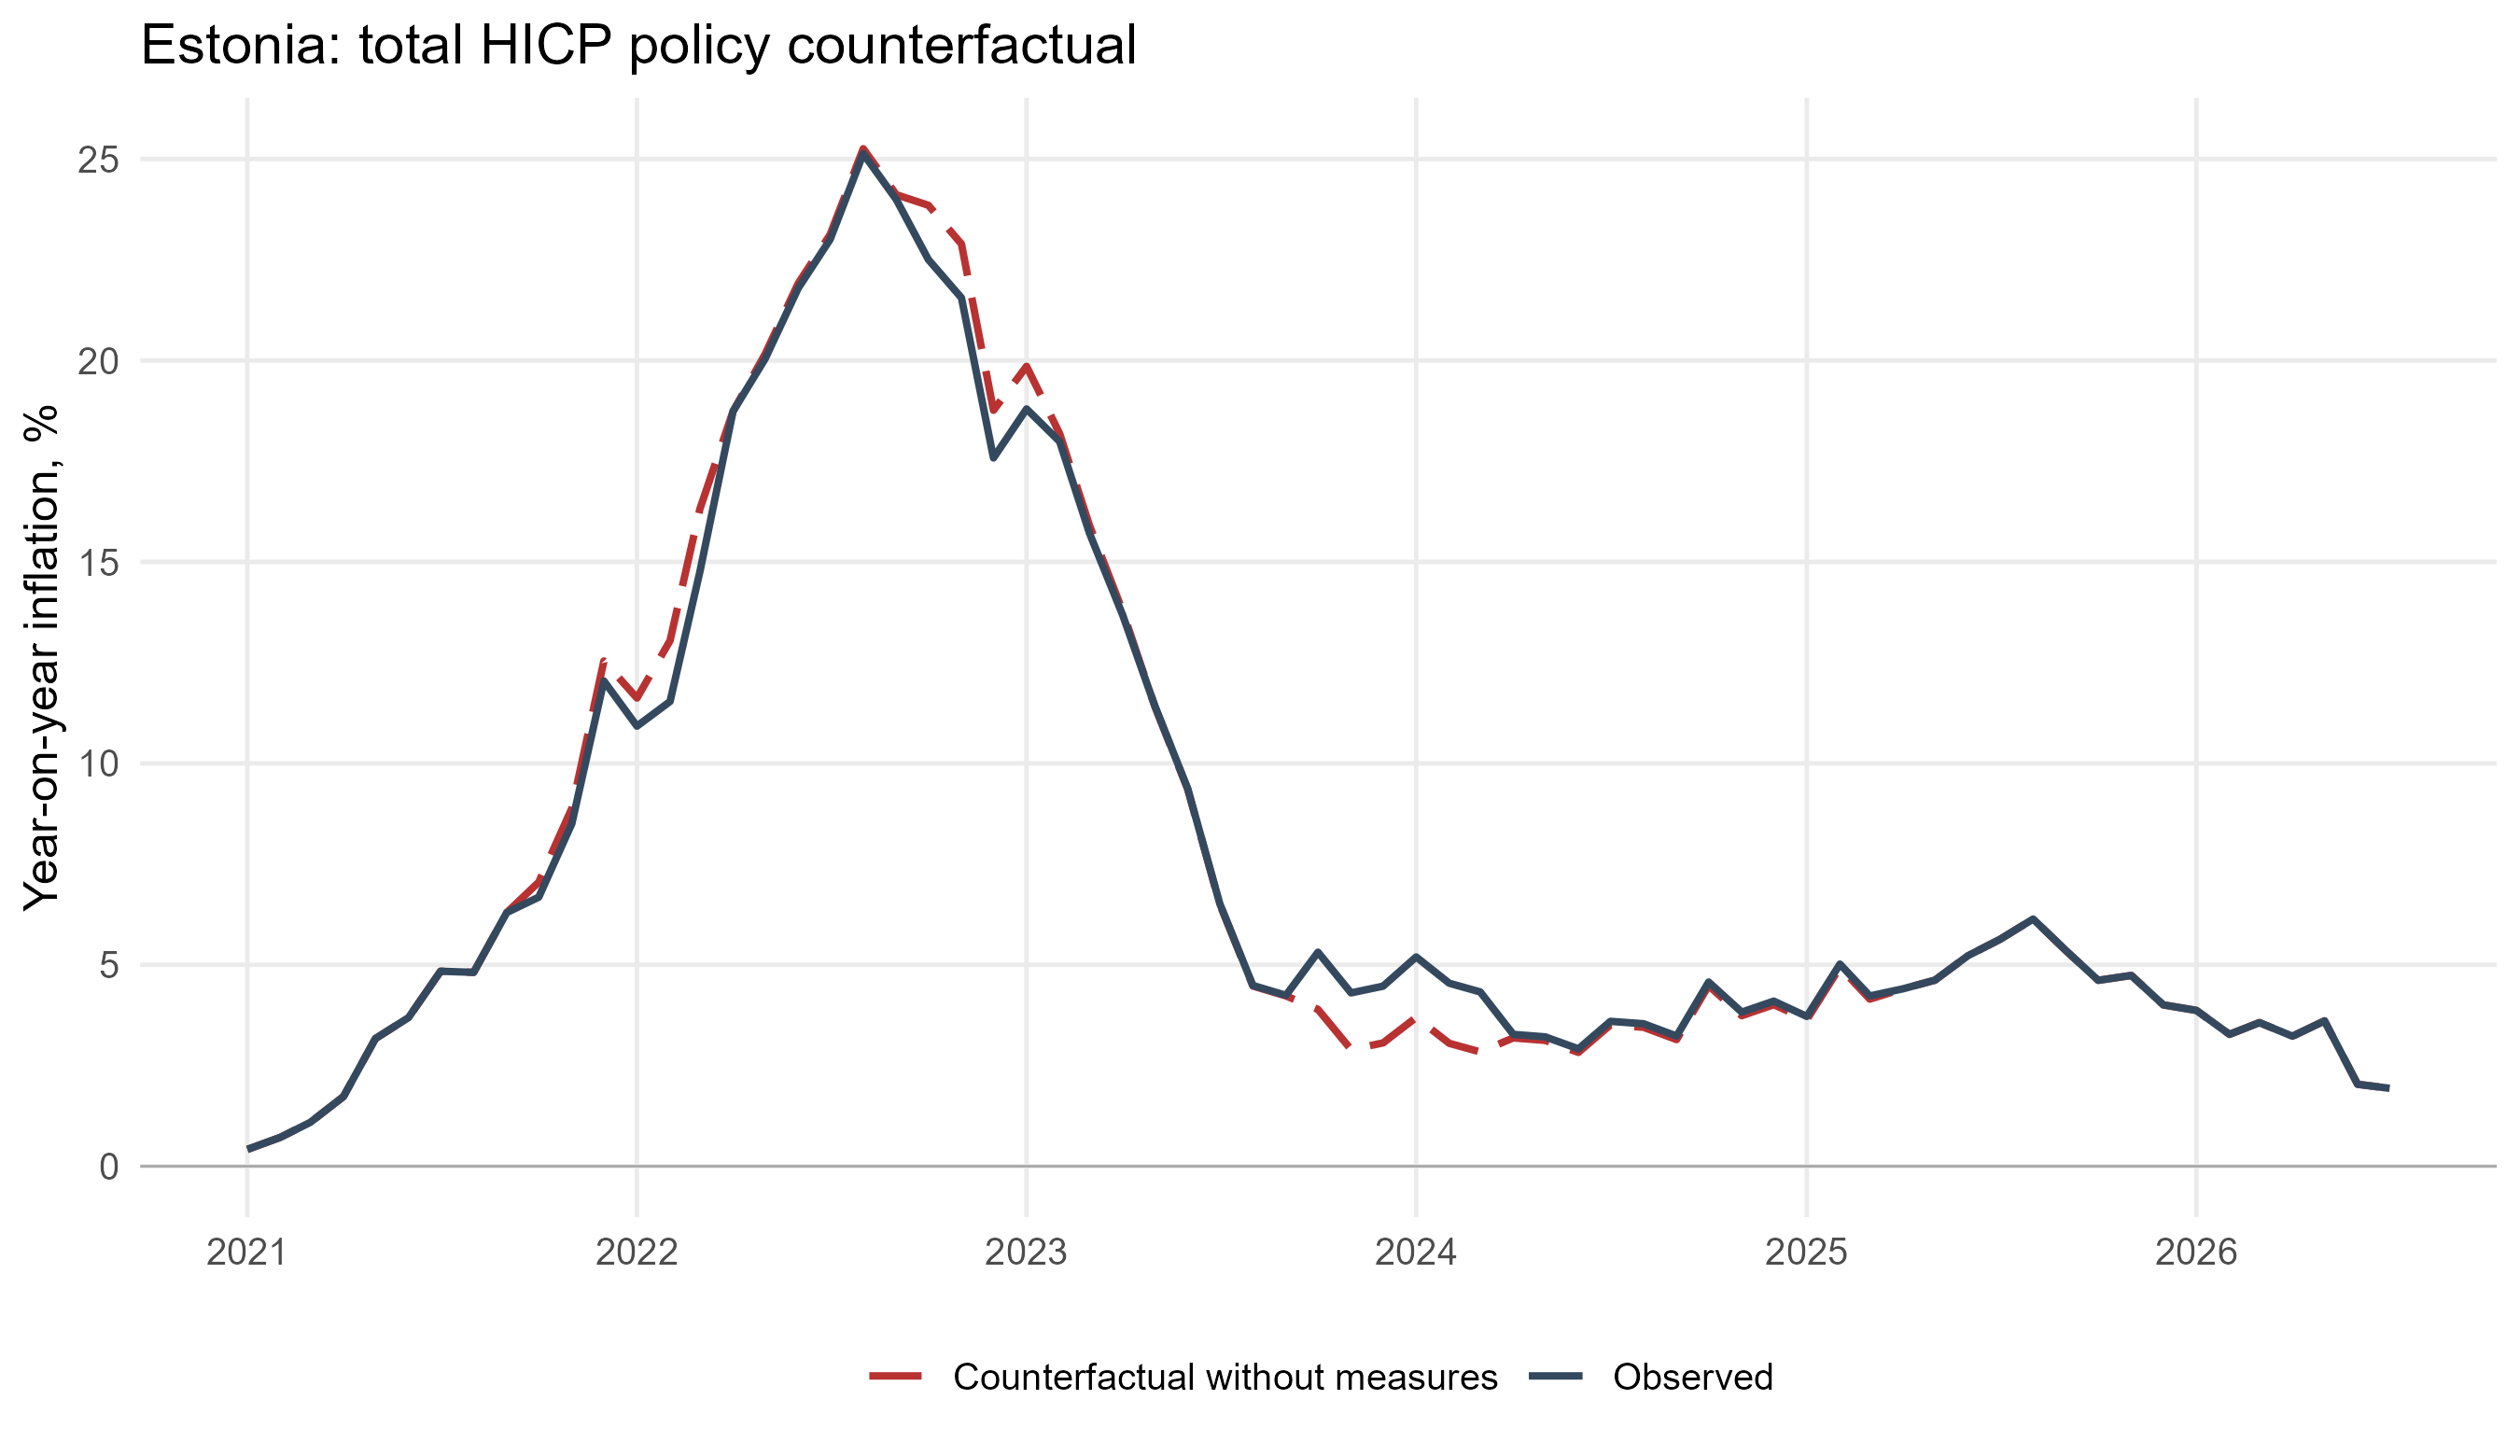
\includegraphics[width=\linewidth,height=0.225\textheight,keepaspectratio]{fig/policy_total_cpi_counterfactual_inflation_EE_estonia.png}\\[-0.4em]\textbf{(e) Estonia}
\end{minipage}\hfill
\begin{minipage}[t]{0.485\textwidth}\centering
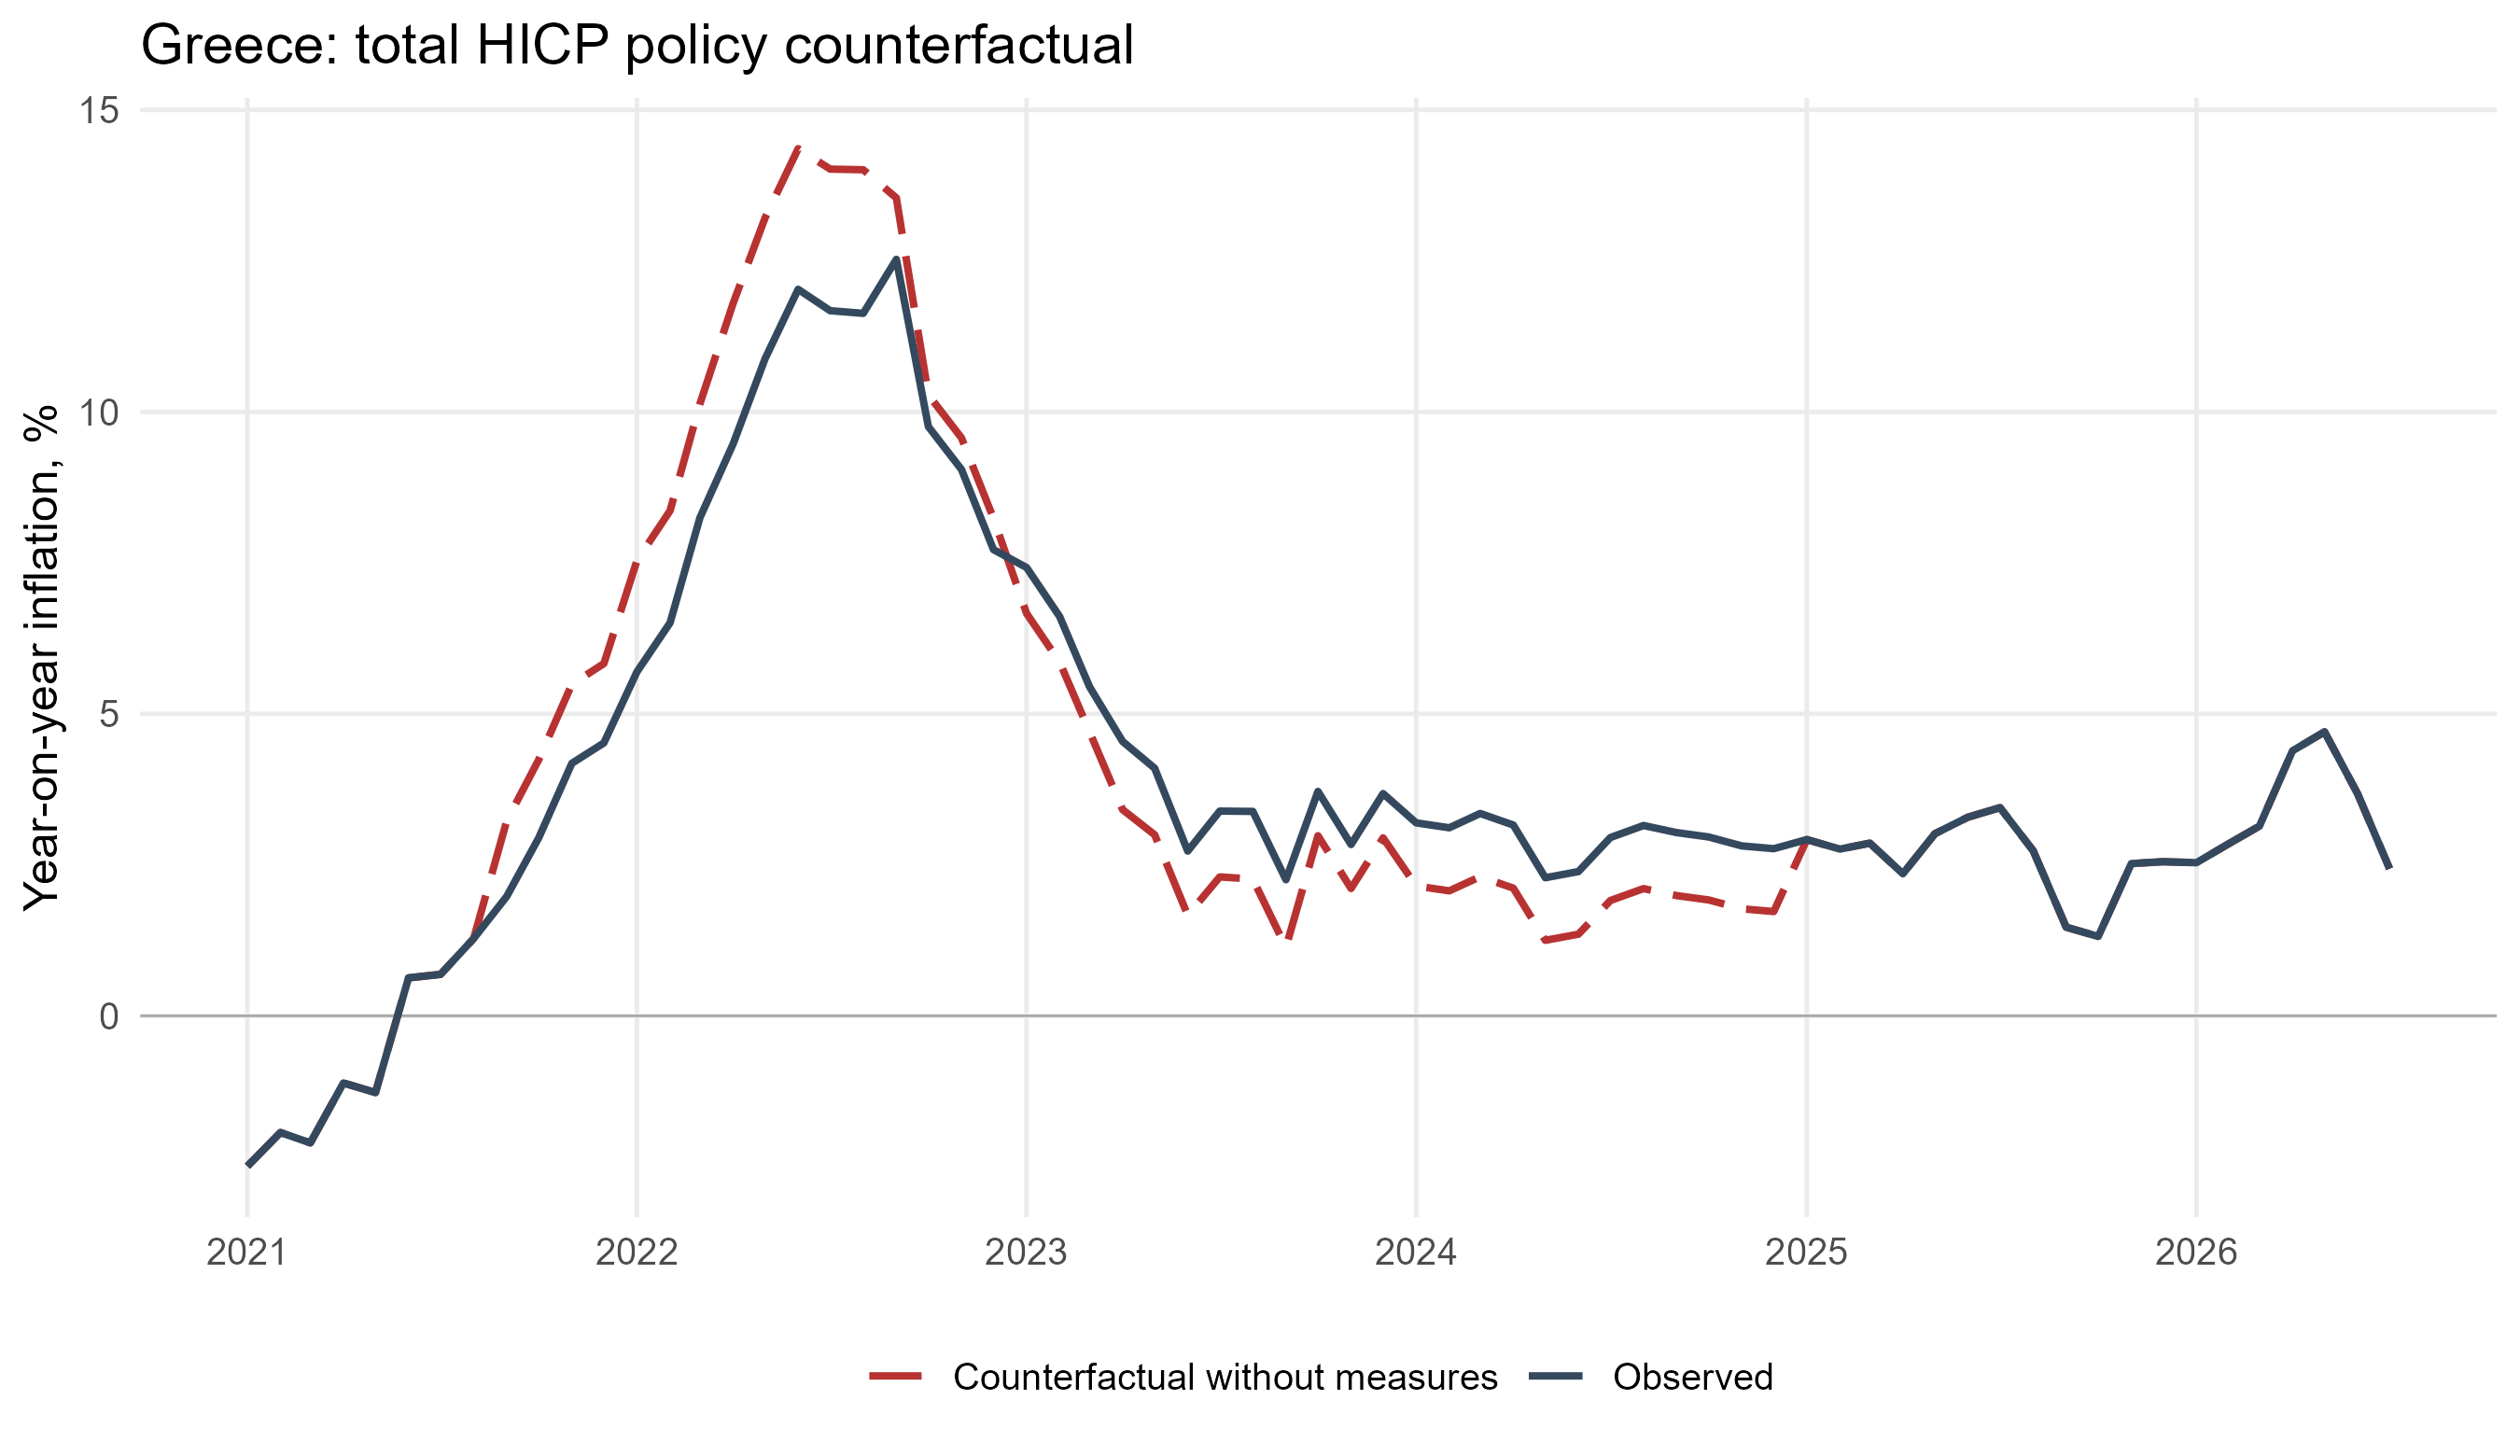
\includegraphics[width=\linewidth,height=0.225\textheight,keepaspectratio]{fig/policy_total_cpi_counterfactual_inflation_EL_greece.png}\\[-0.4em]\textbf{(f) Greece}
\end{minipage}
\caption{Observed and counterfactual inflation: Austria, Belgium, Cyprus, Germany, Estonia, Greece}
\label{fig:country-counterfactuals-1}
\end{figure}
\clearpage

\begin{figure}[H]
\centering
\begin{minipage}[t]{0.485\textwidth}\centering
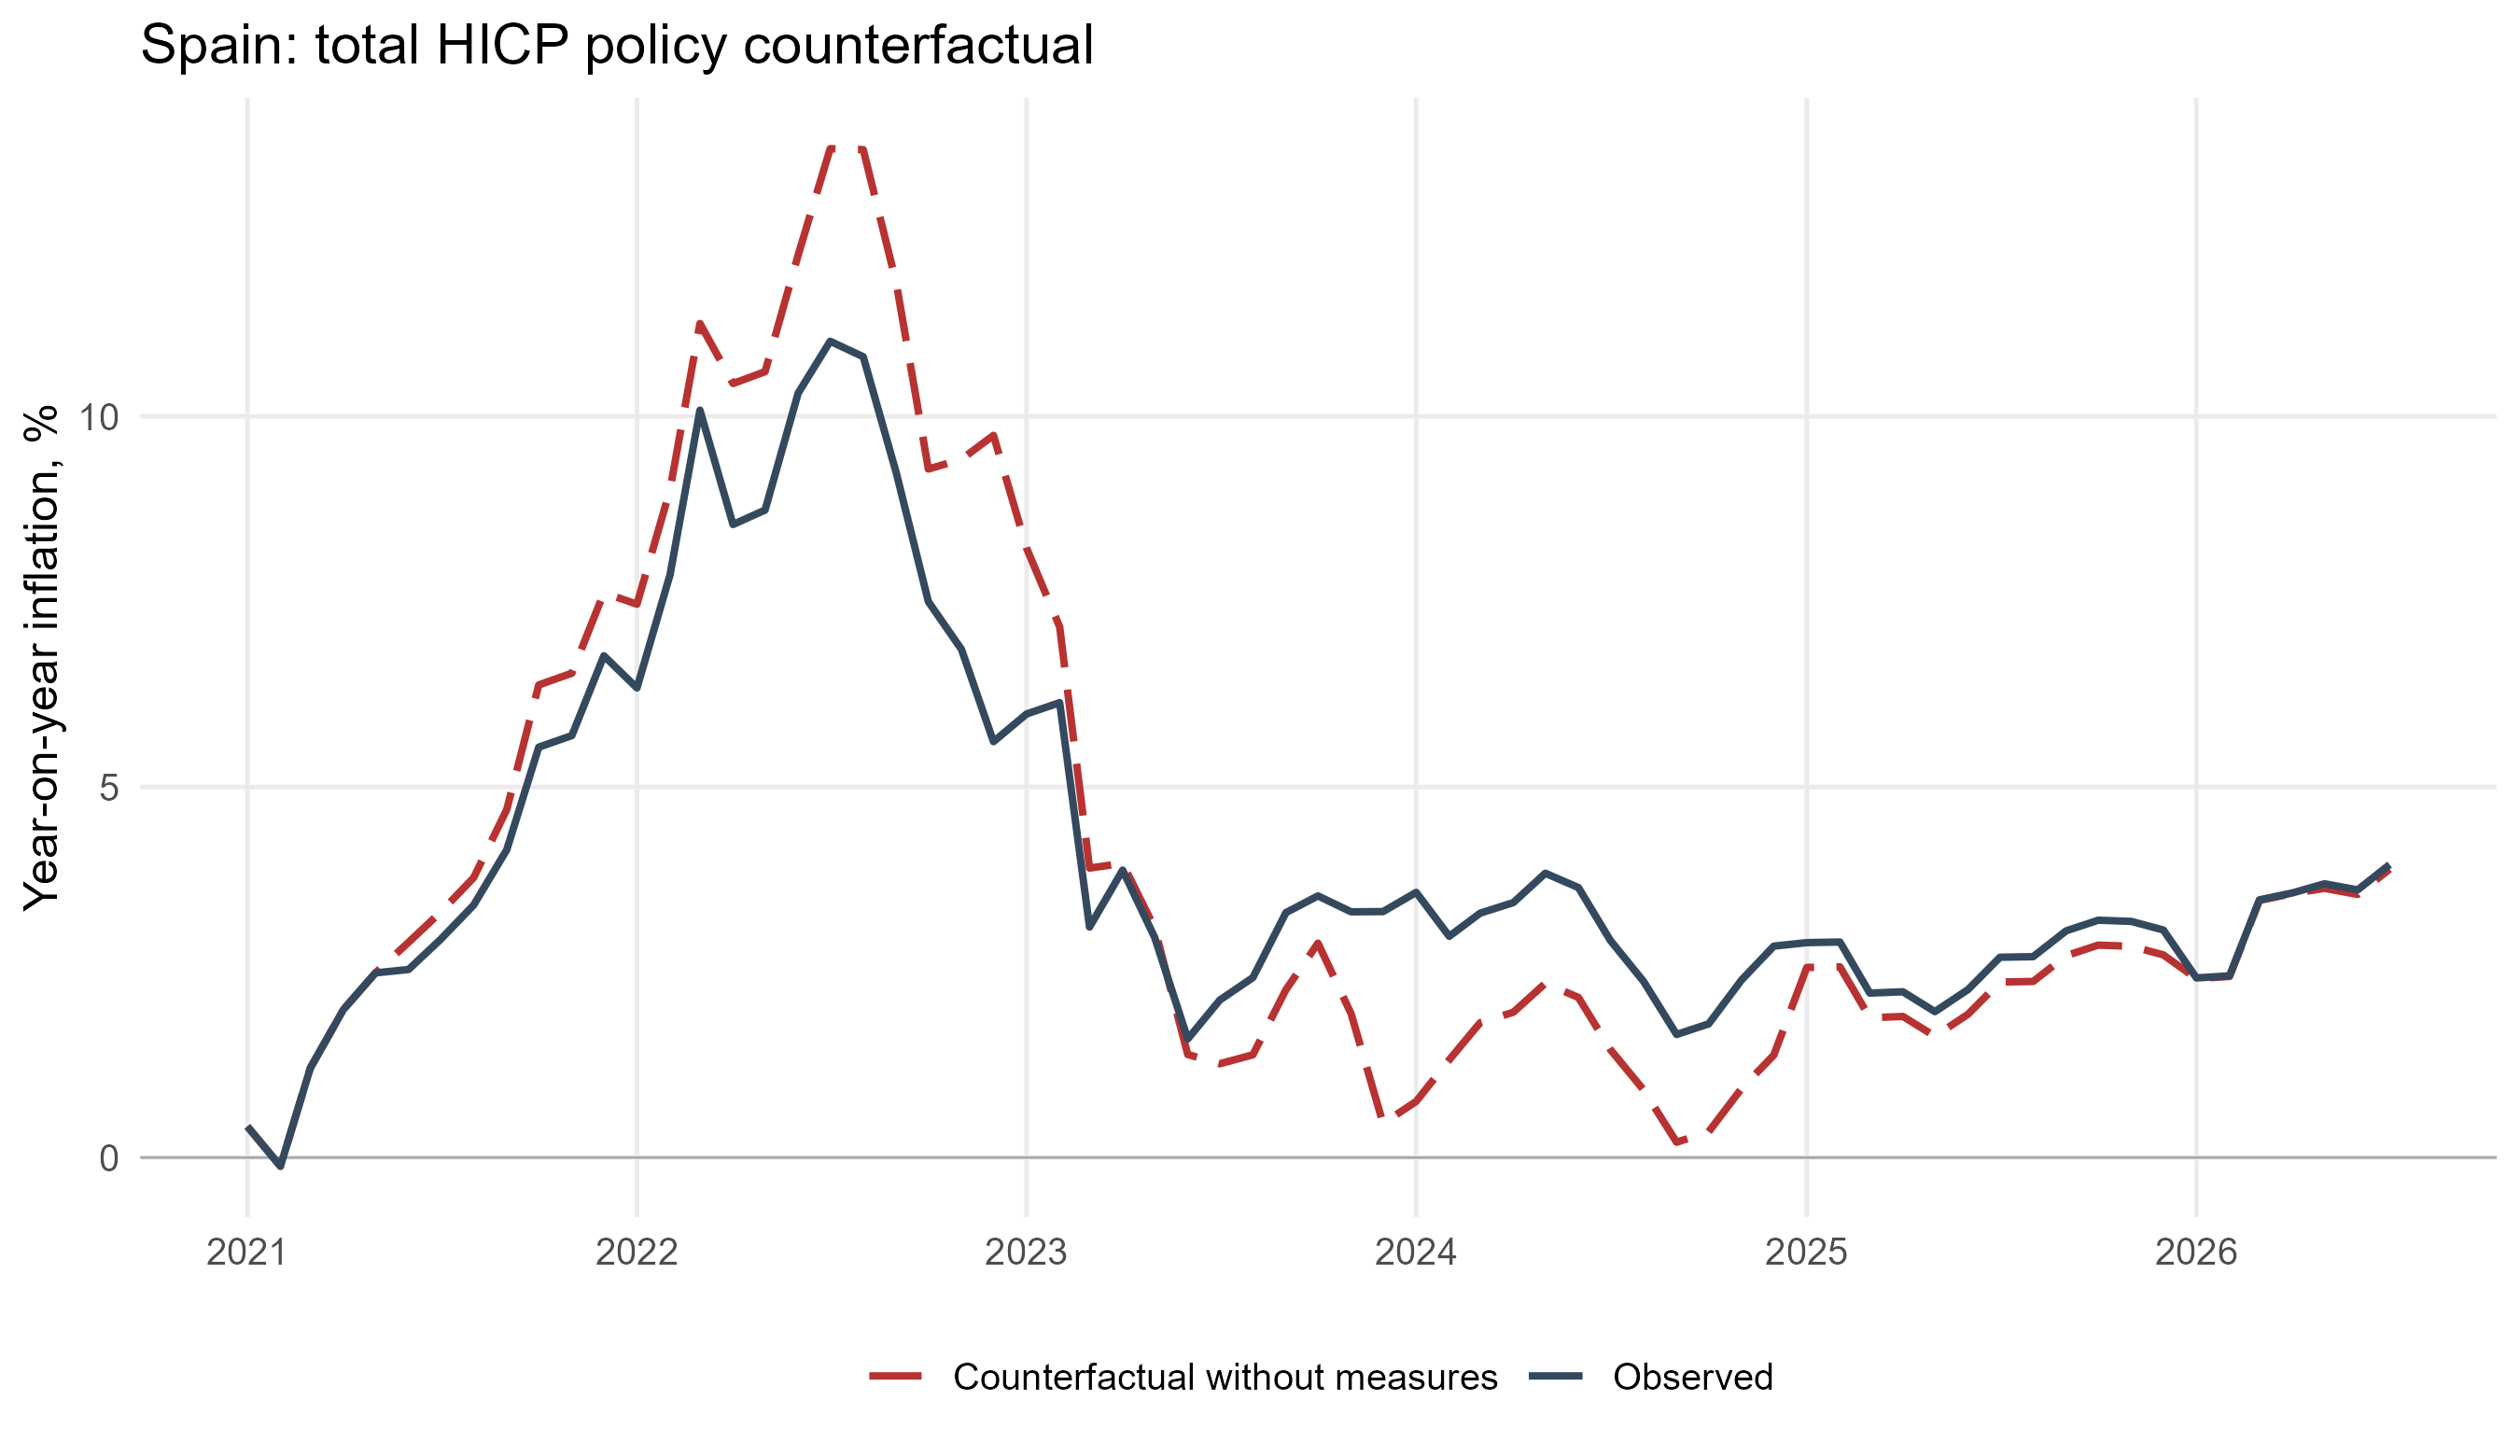
\includegraphics[width=\linewidth,height=0.225\textheight,keepaspectratio]{fig/policy_total_cpi_counterfactual_inflation_ES_spain.png}\\[-0.4em]\textbf{(a) Spain}
\end{minipage}\hfill
\begin{minipage}[t]{0.485\textwidth}\centering
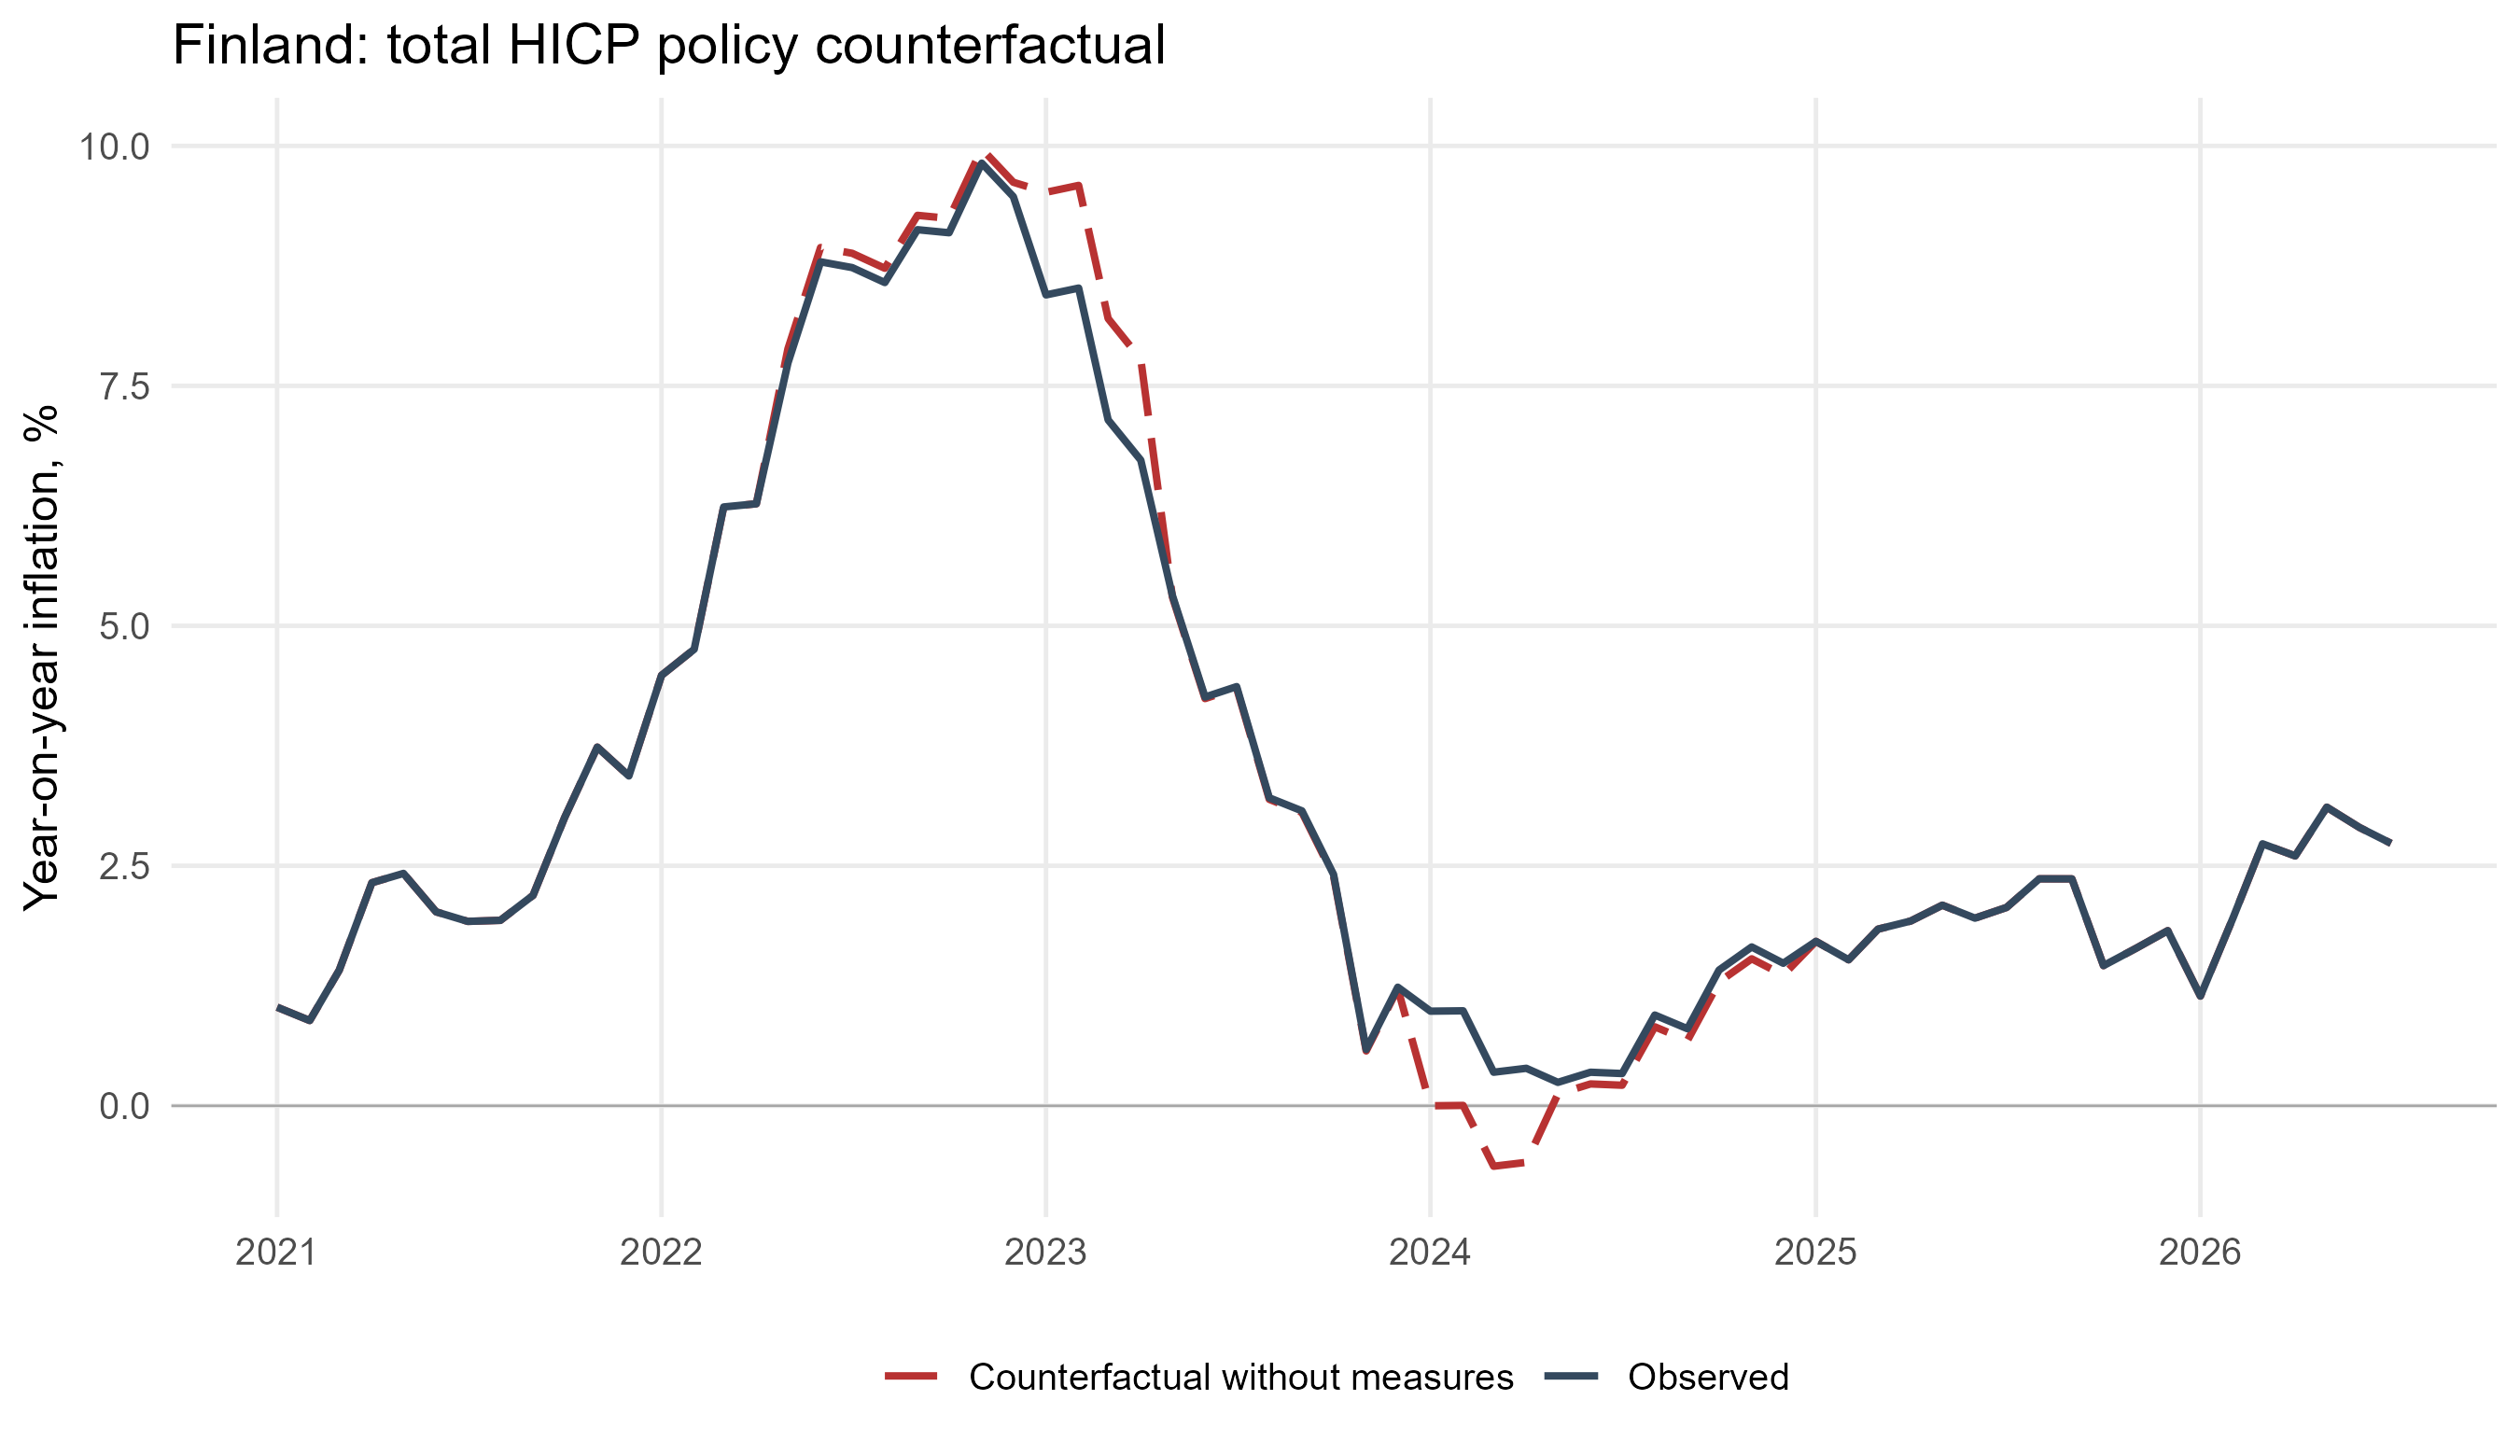
\includegraphics[width=\linewidth,height=0.225\textheight,keepaspectratio]{fig/policy_total_cpi_counterfactual_inflation_FI_finland.png}\\[-0.4em]\textbf{(b) Finland}
\end{minipage}

\vspace{0.25em}
\begin{minipage}[t]{0.485\textwidth}\centering
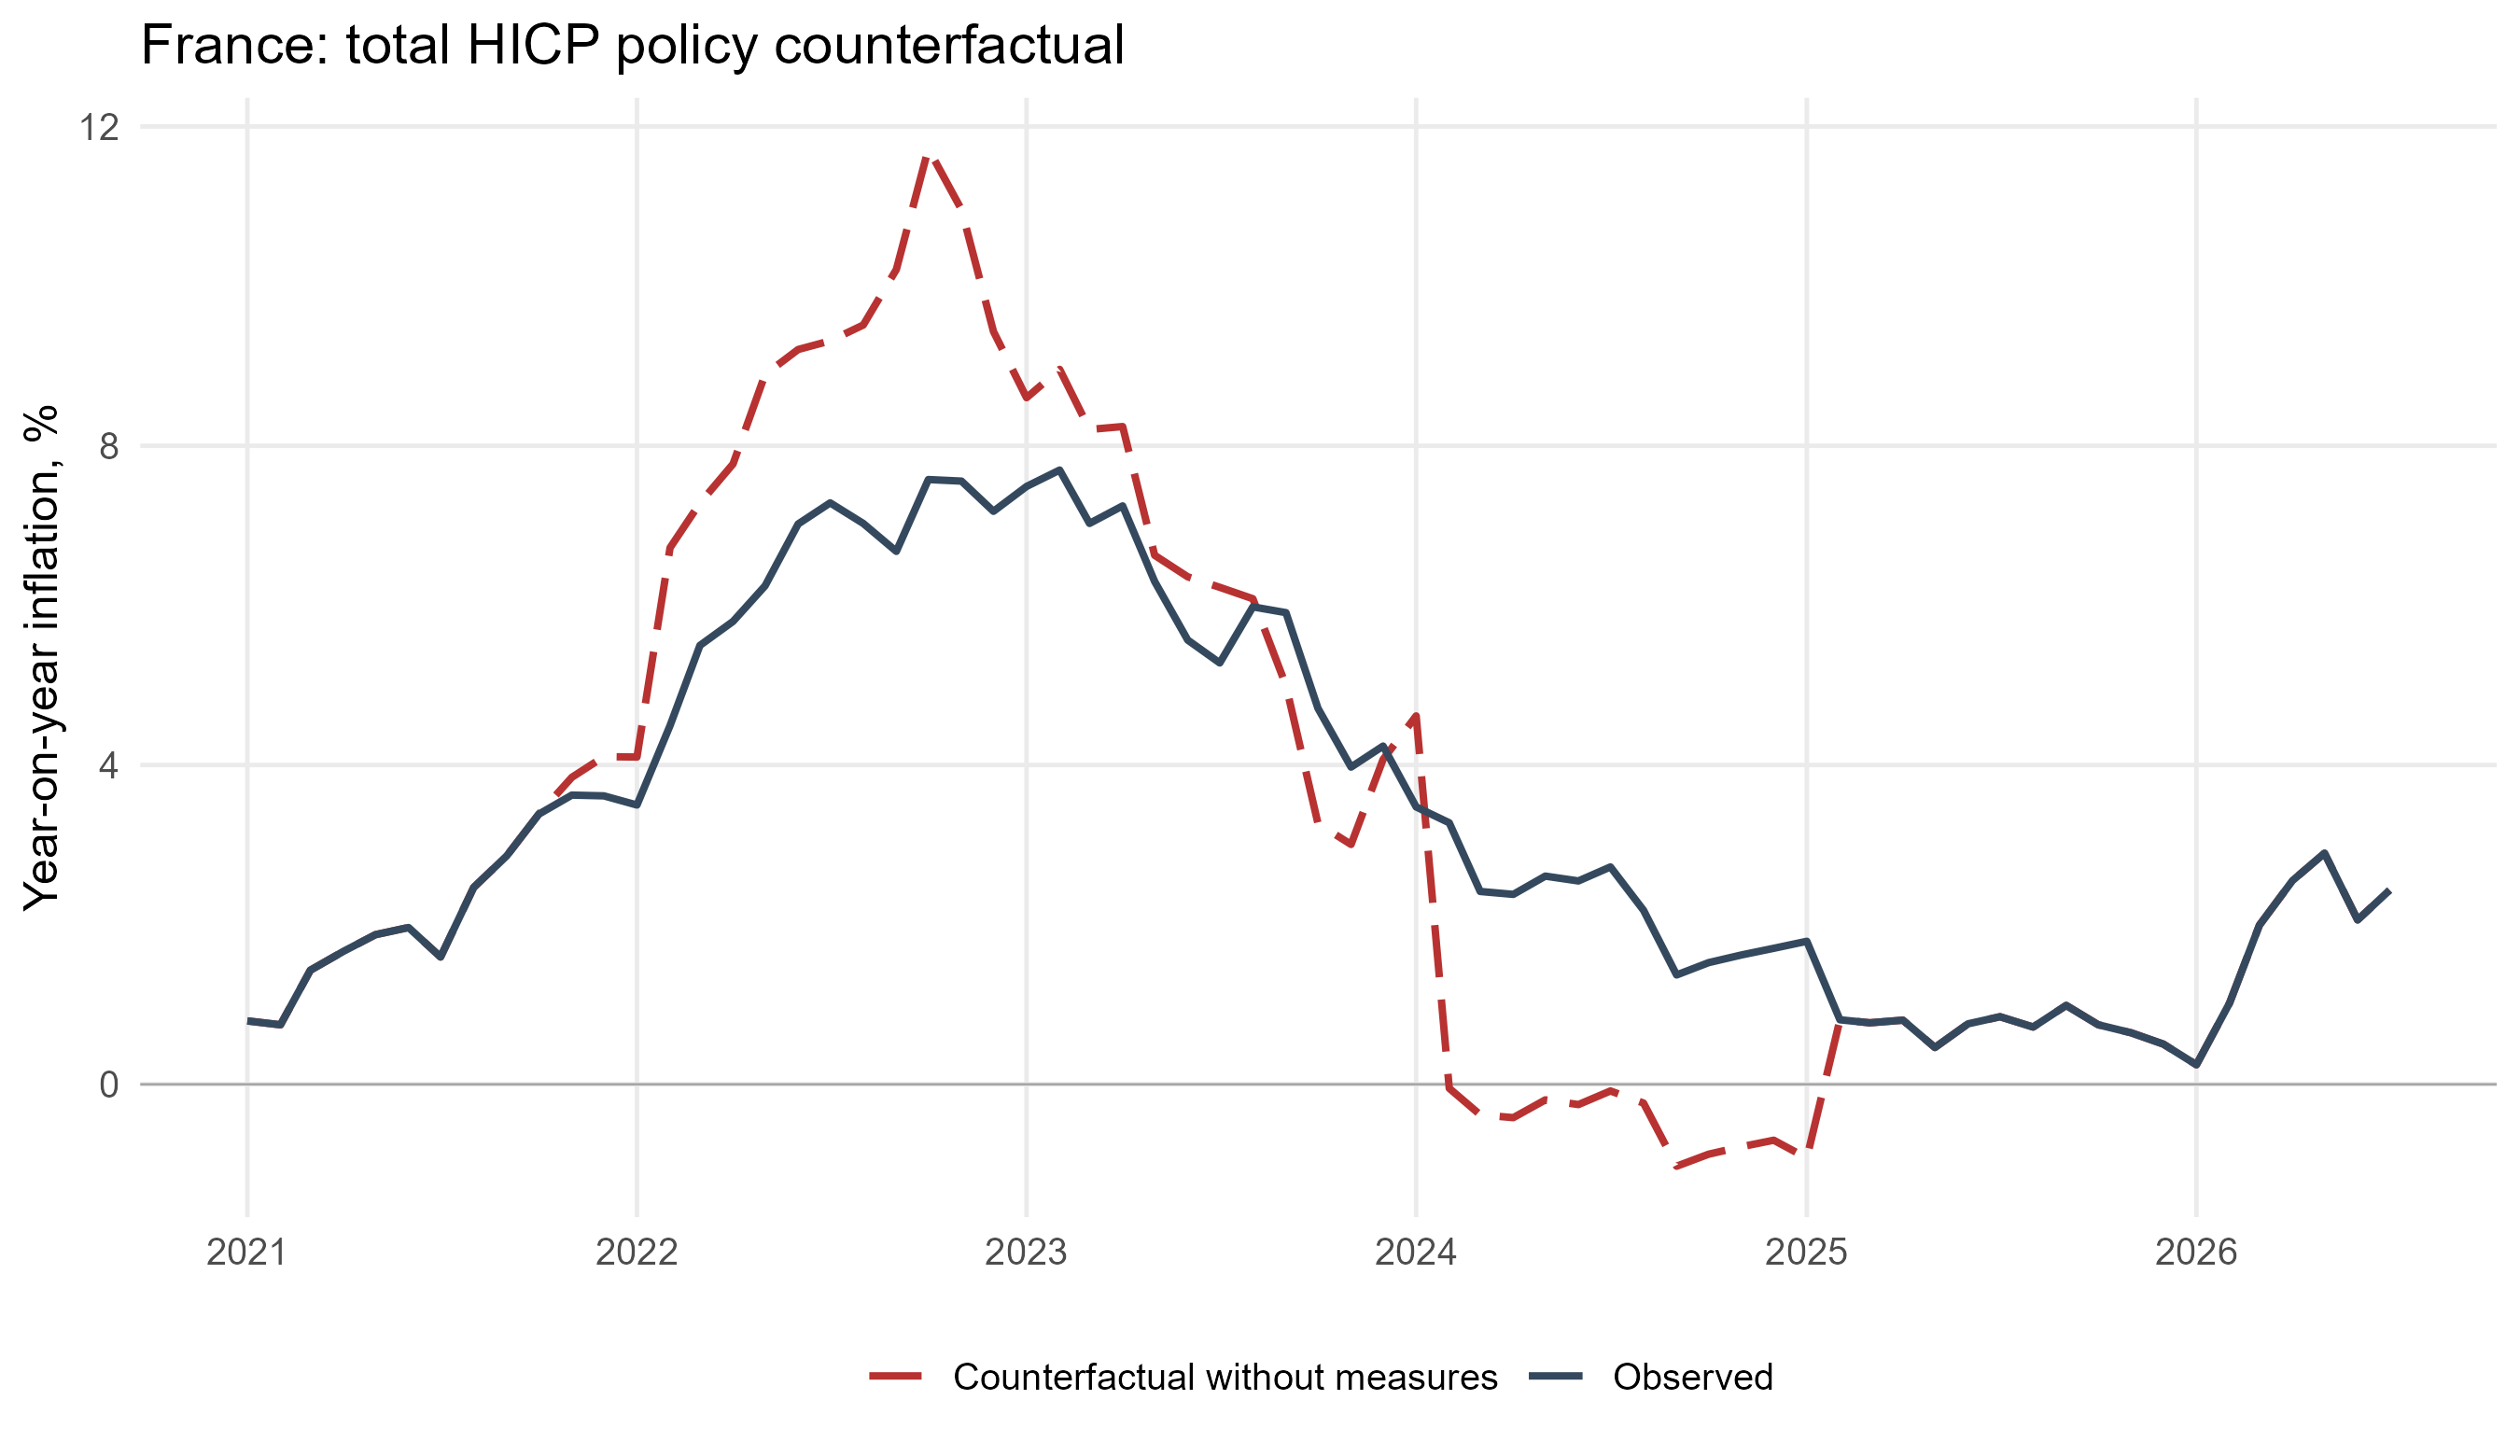
\includegraphics[width=\linewidth,height=0.225\textheight,keepaspectratio]{fig/policy_total_cpi_counterfactual_inflation_FR_france.png}\\[-0.4em]\textbf{(c) France}
\end{minipage}\hfill
\begin{minipage}[t]{0.485\textwidth}\centering
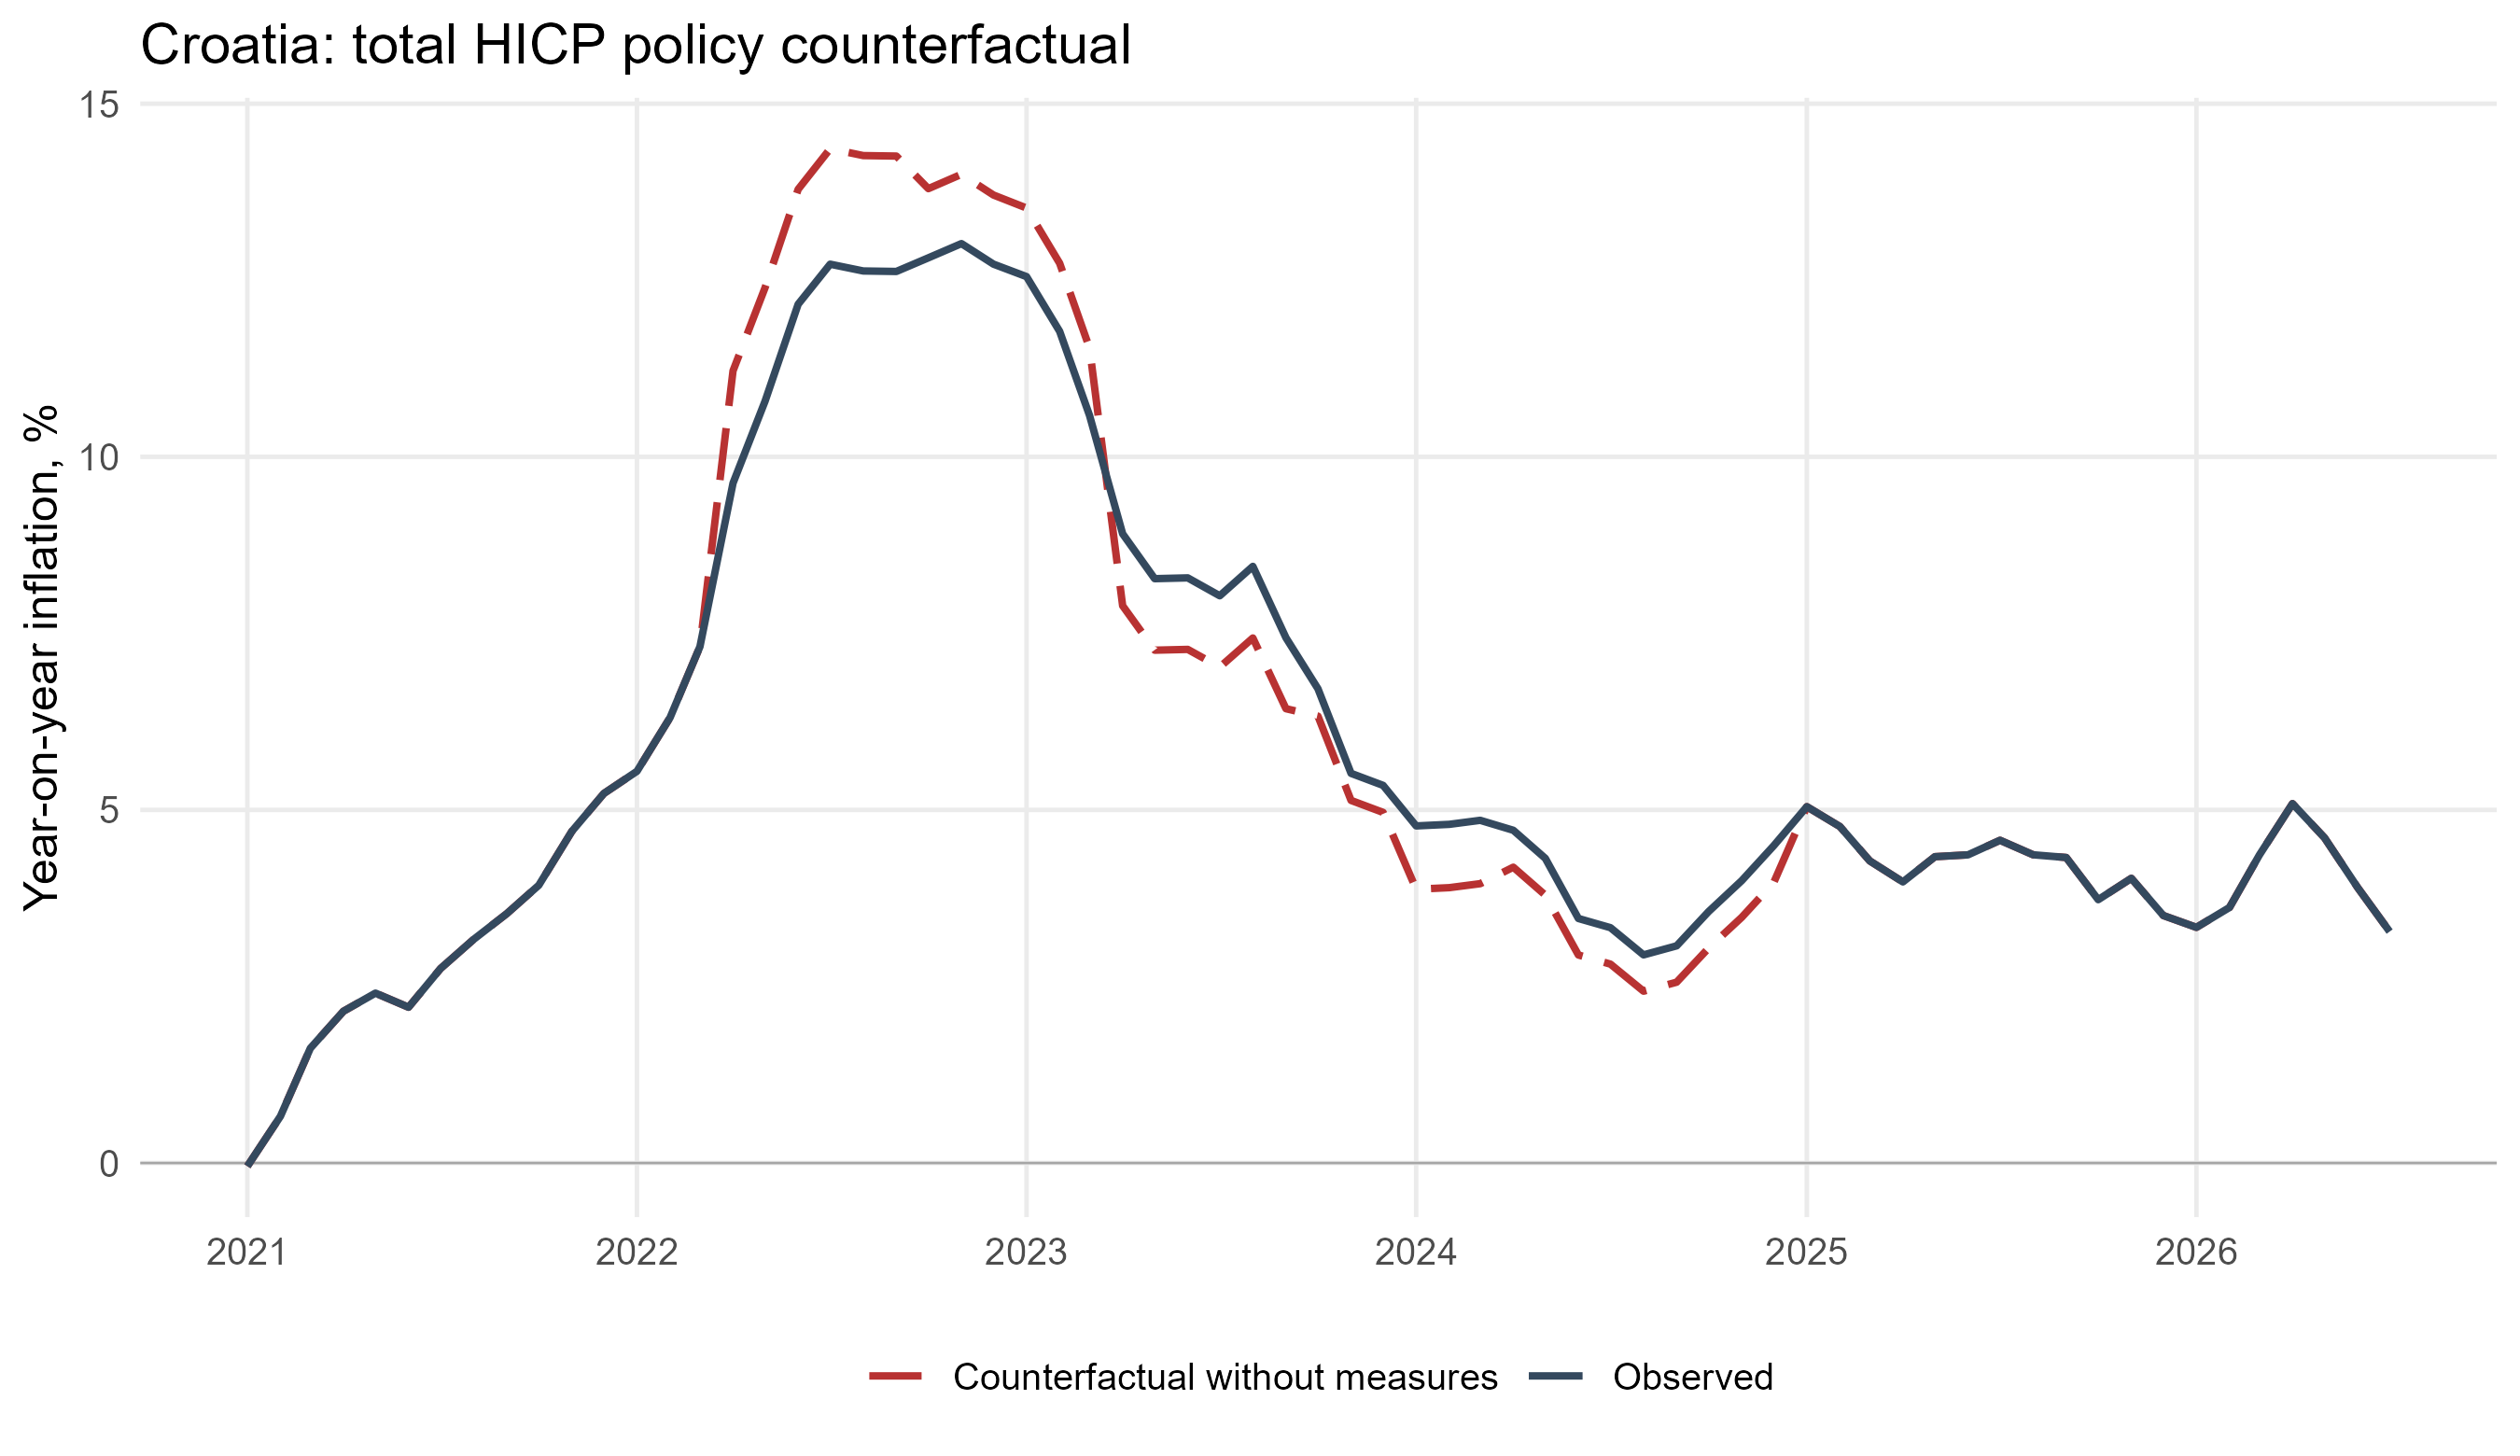
\includegraphics[width=\linewidth,height=0.225\textheight,keepaspectratio]{fig/policy_total_cpi_counterfactual_inflation_HR_croatia.png}\\[-0.4em]\textbf{(d) Croatia}
\end{minipage}

\vspace{0.25em}
\begin{minipage}[t]{0.485\textwidth}\centering
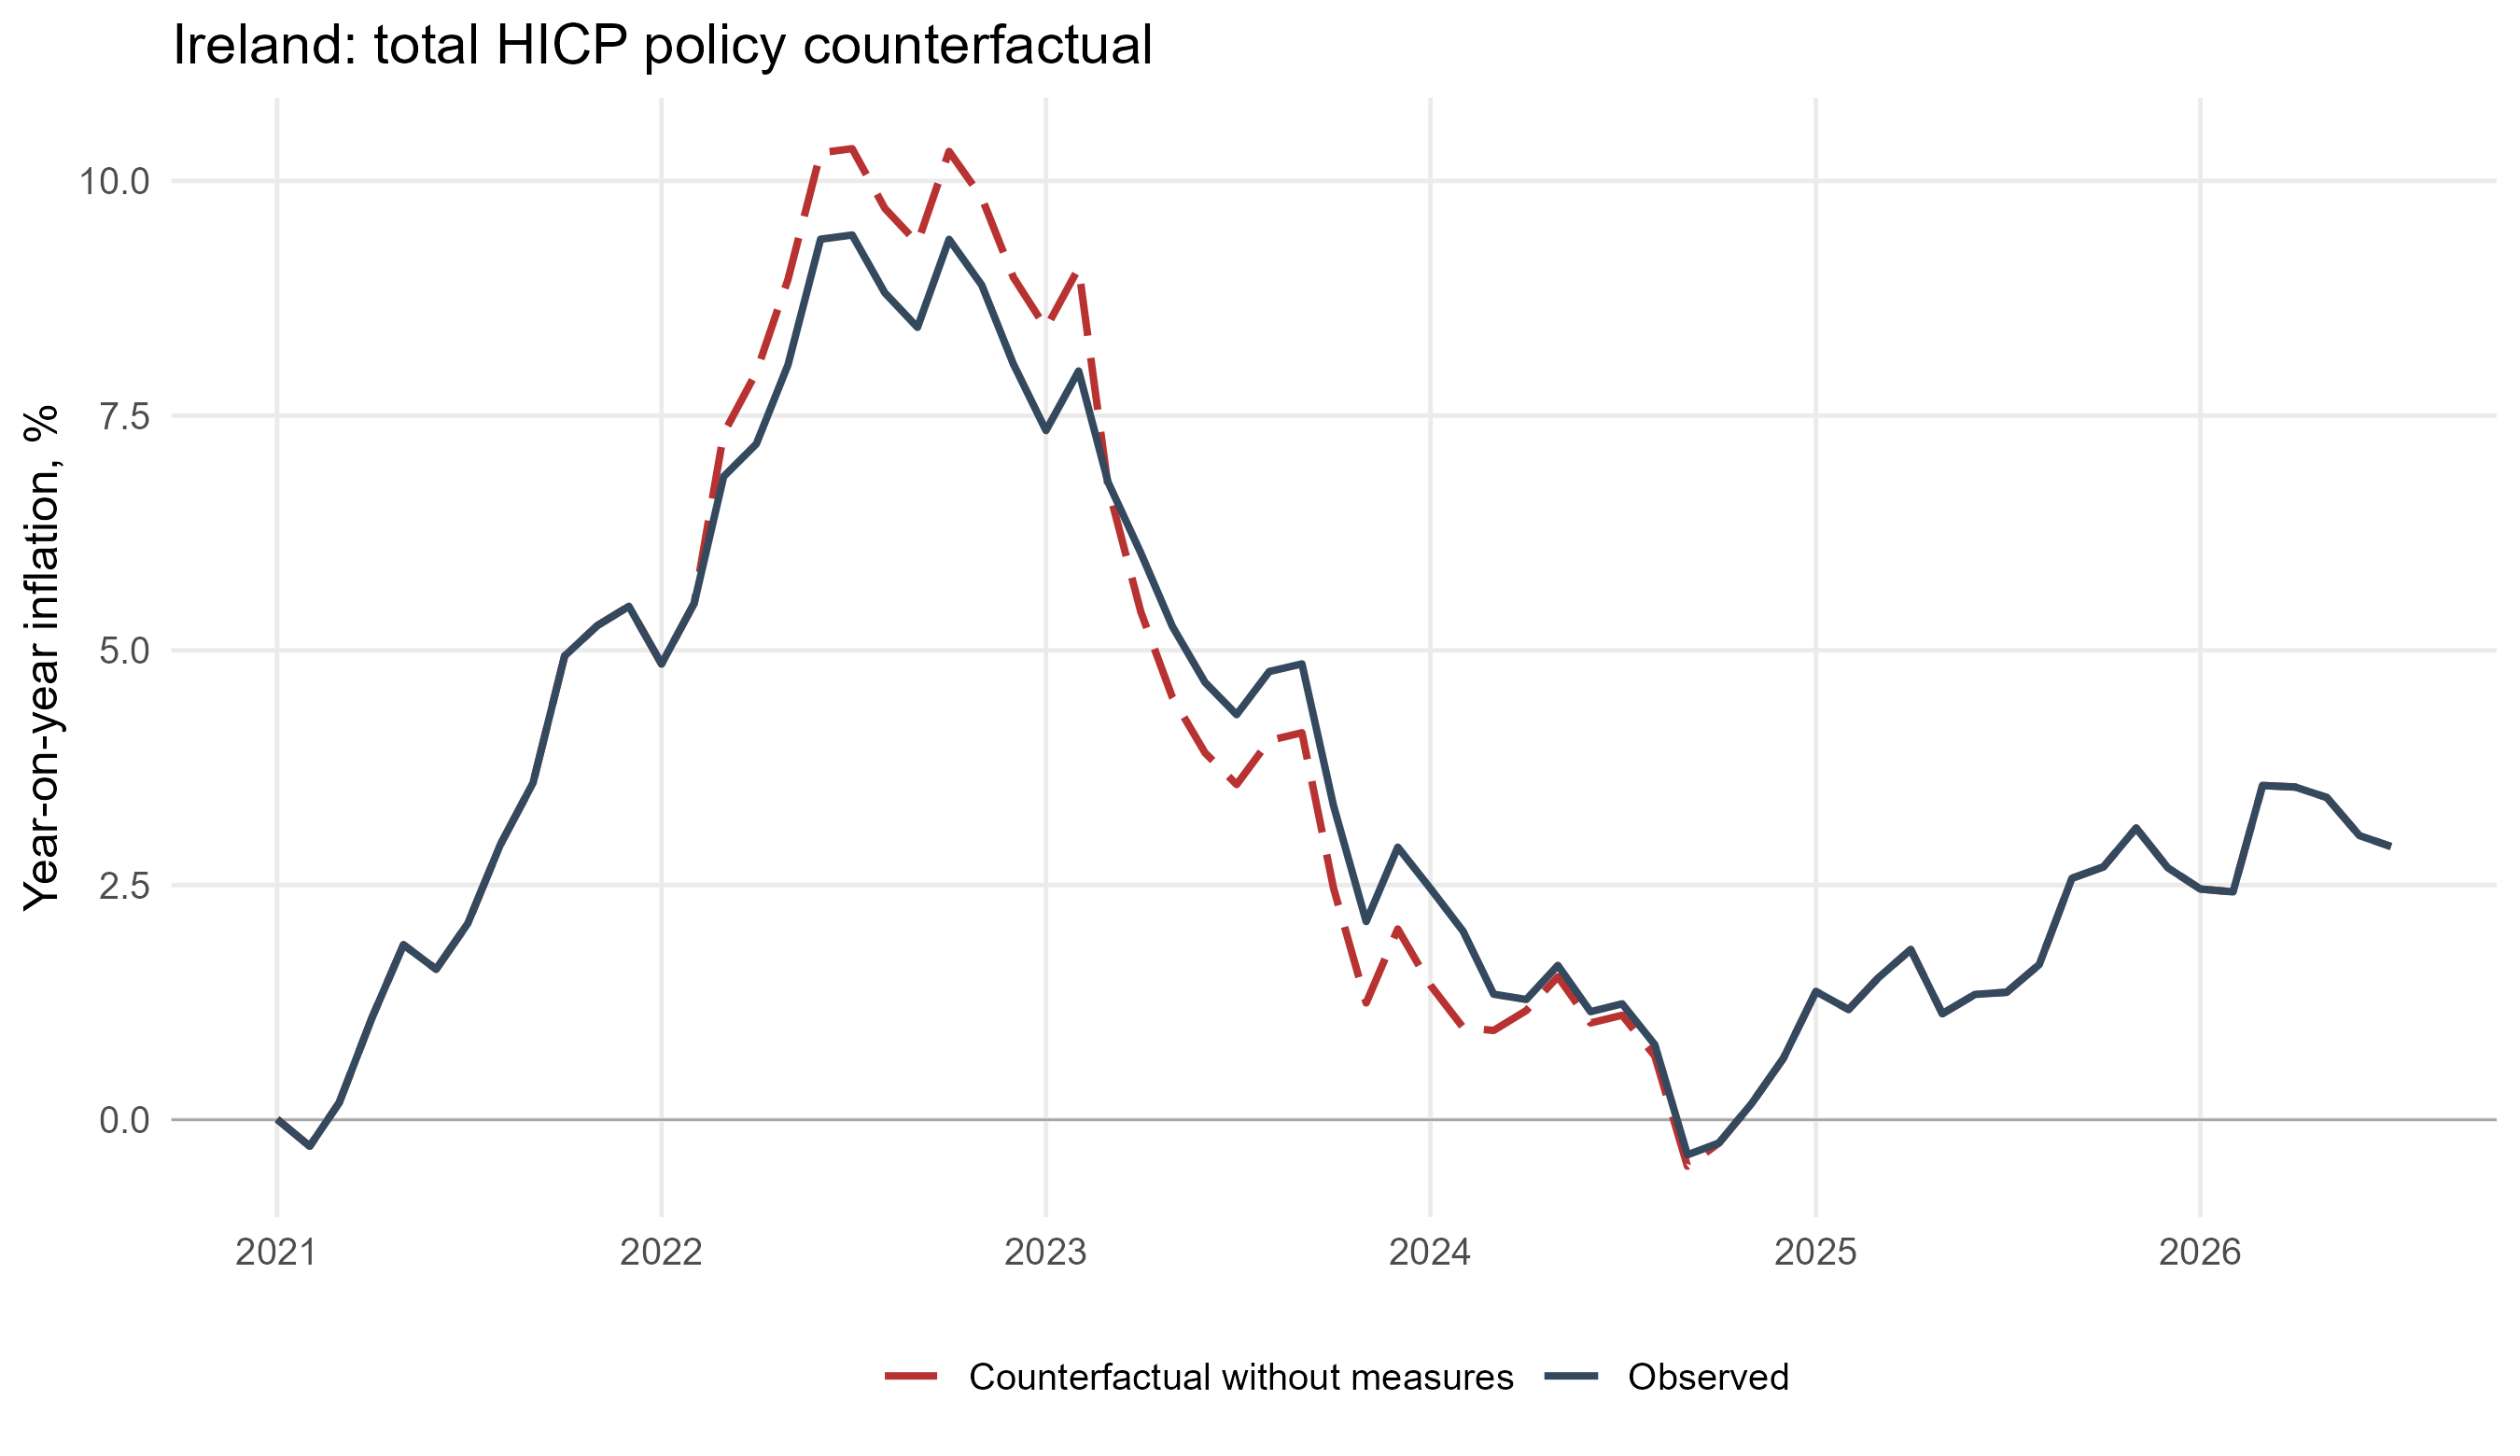
\includegraphics[width=\linewidth,height=0.225\textheight,keepaspectratio]{fig/policy_total_cpi_counterfactual_inflation_IE_ireland.png}\\[-0.4em]\textbf{(e) Ireland}
\end{minipage}\hfill
\begin{minipage}[t]{0.485\textwidth}\centering
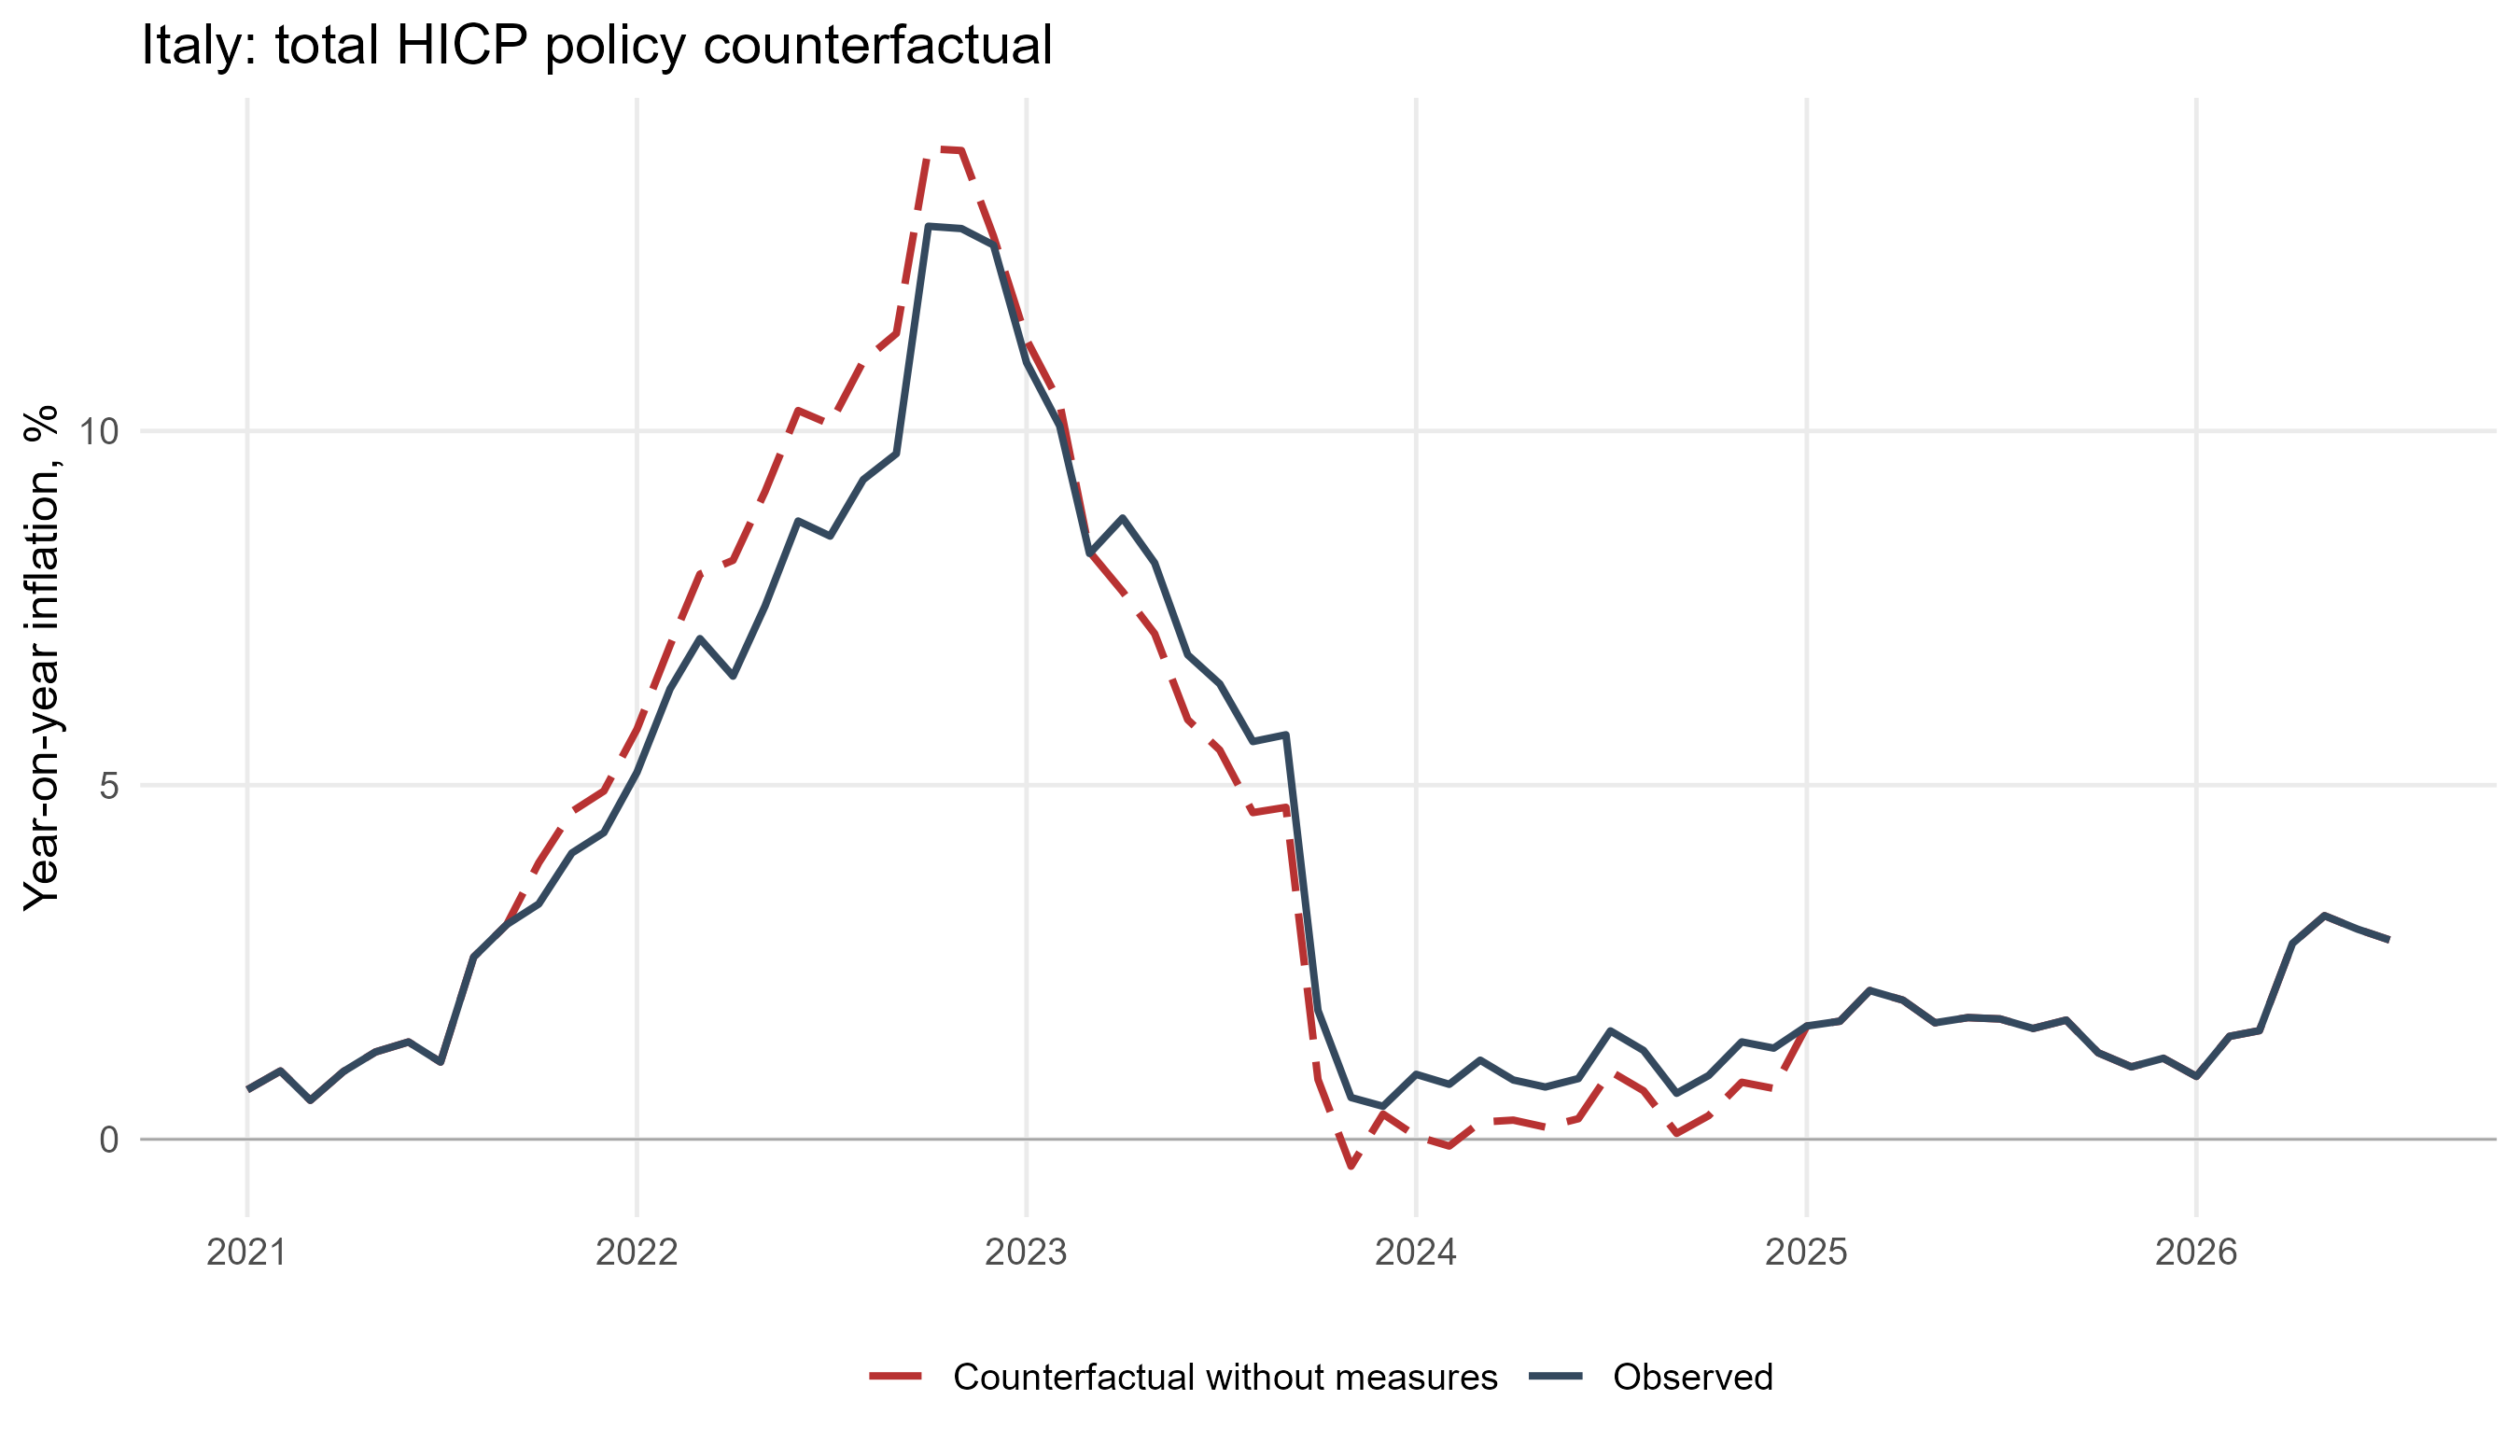
\includegraphics[width=\linewidth,height=0.225\textheight,keepaspectratio]{fig/policy_total_cpi_counterfactual_inflation_IT_italy.png}\\[-0.4em]\textbf{(f) Italy}
\end{minipage}
\caption{Observed and counterfactual inflation: Spain, Finland, France, Croatia, Ireland, Italy}
\label{fig:country-counterfactuals-2}
\end{figure}
\clearpage

\begin{figure}[H]
\centering
\begin{minipage}[t]{0.485\textwidth}\centering
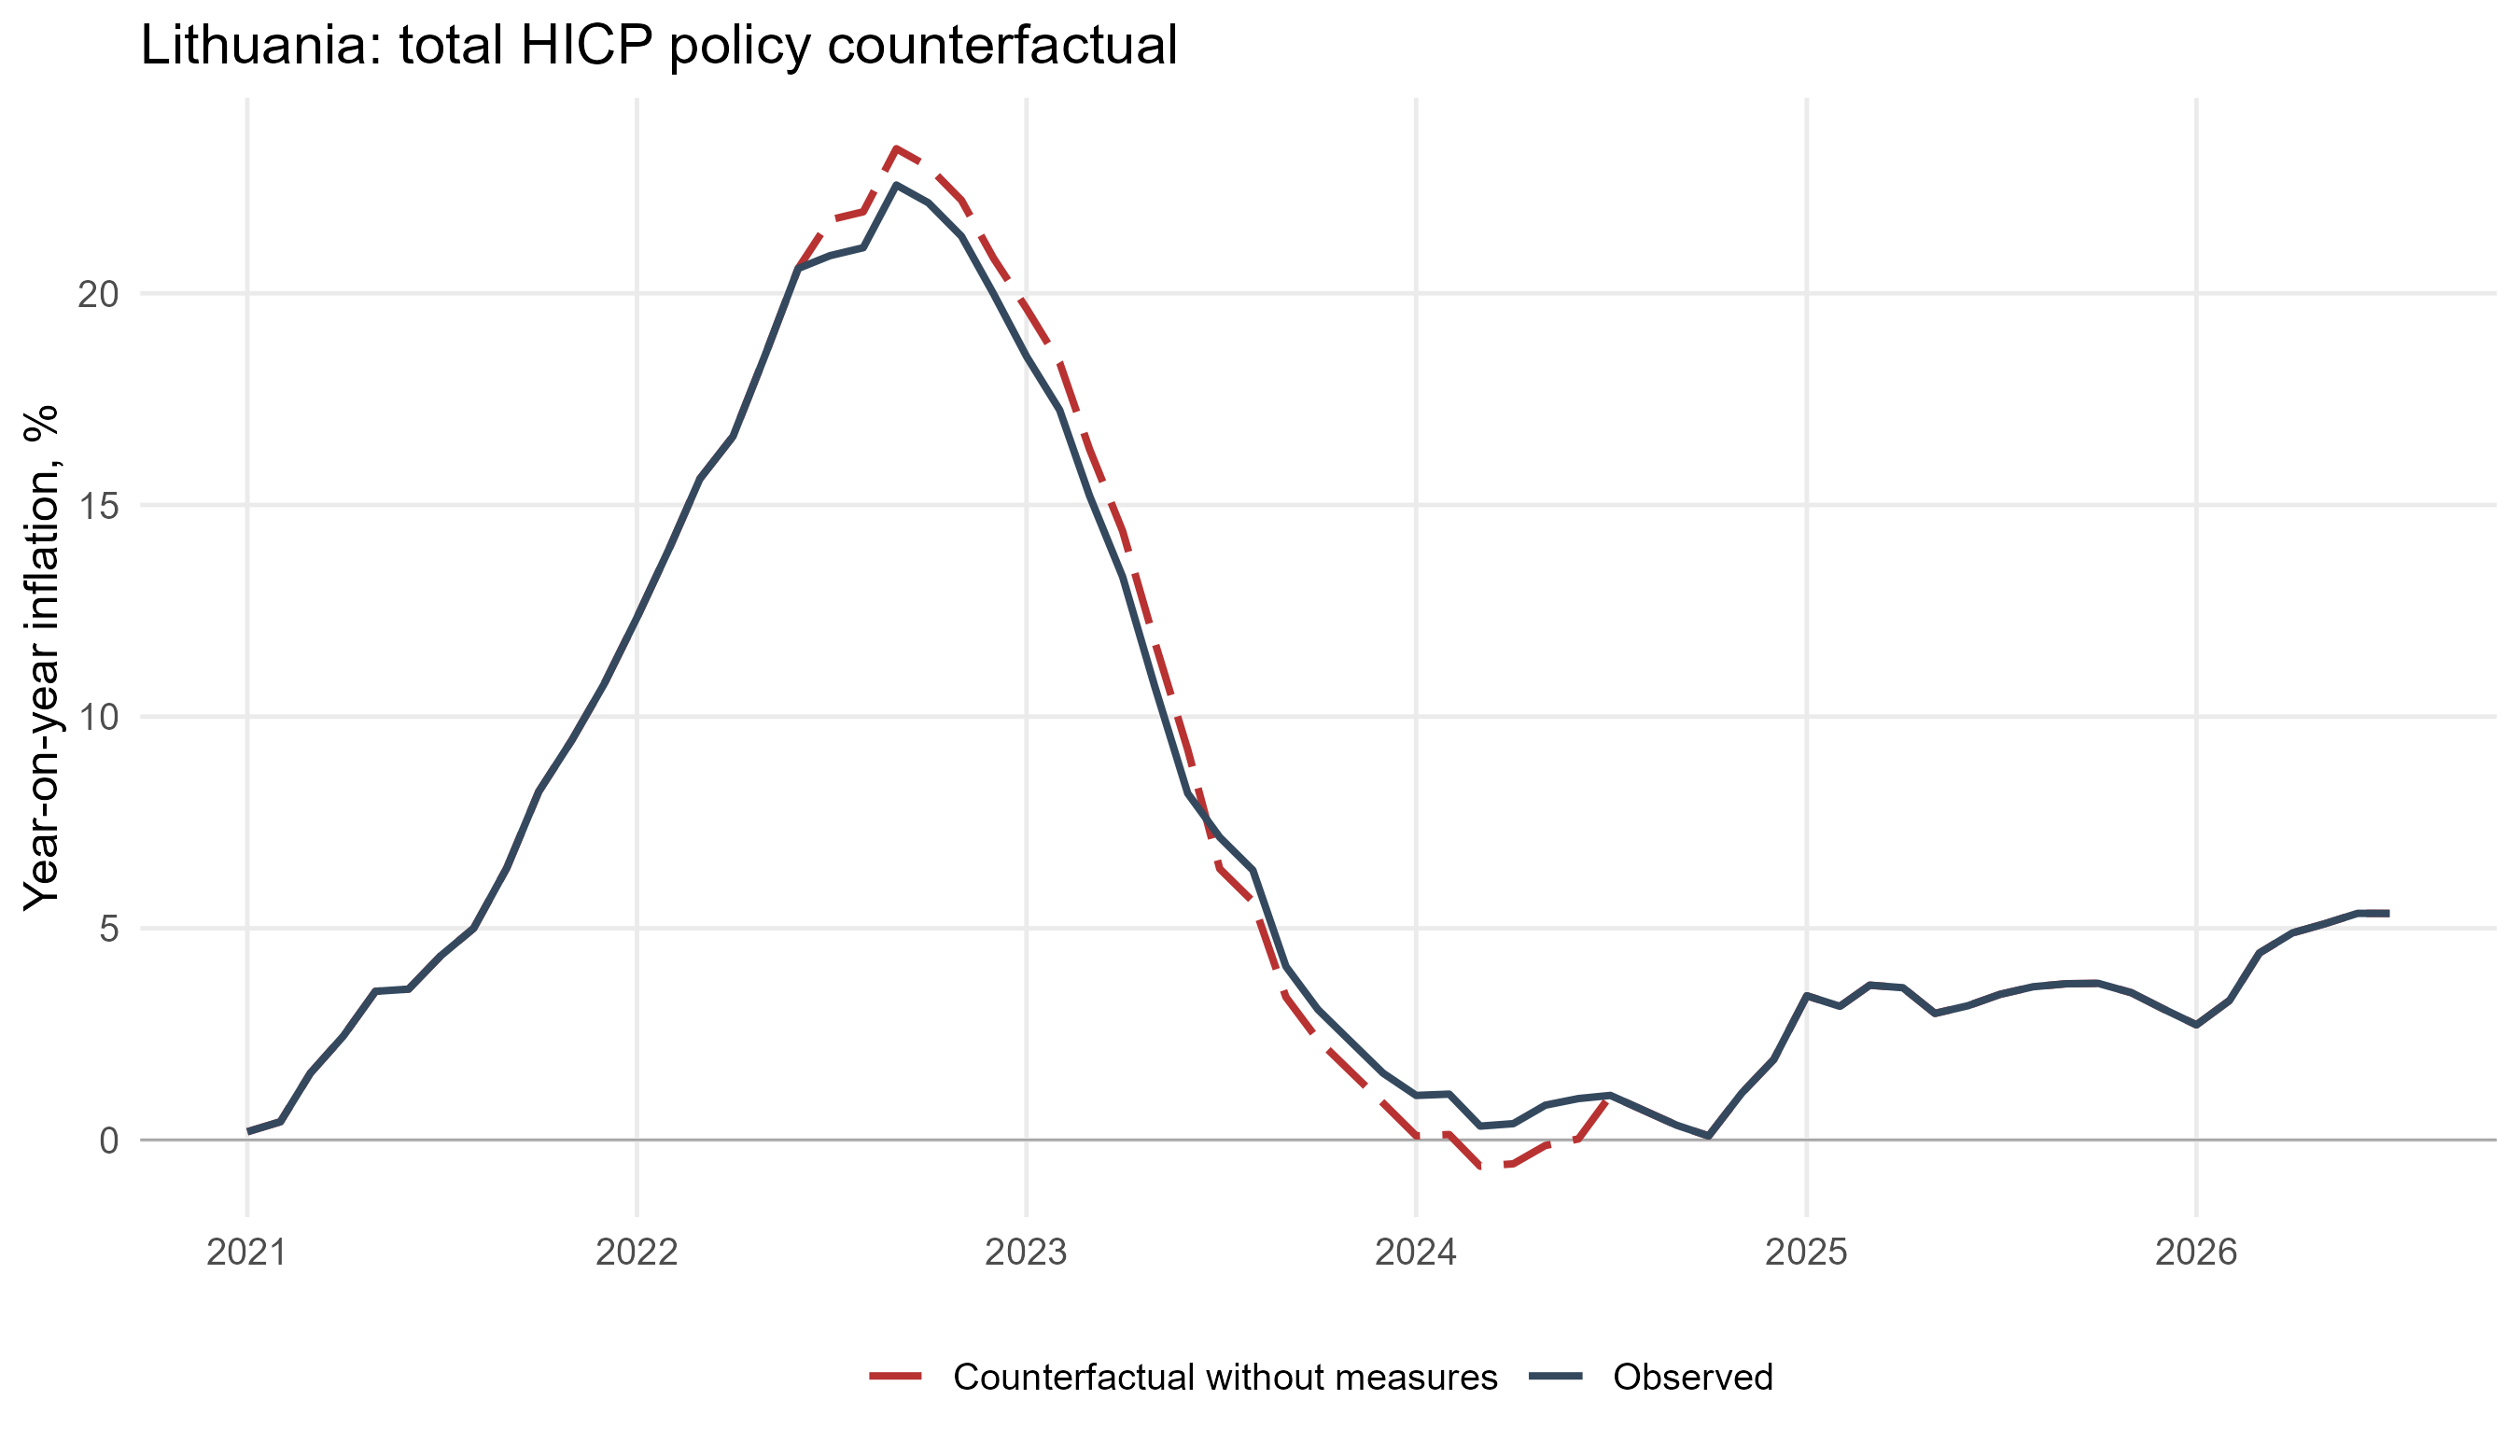
\includegraphics[width=\linewidth,height=0.225\textheight,keepaspectratio]{fig/policy_total_cpi_counterfactual_inflation_LT_lithuania.png}\\[-0.4em]\textbf{(a) Lithuania}
\end{minipage}\hfill
\begin{minipage}[t]{0.485\textwidth}\centering
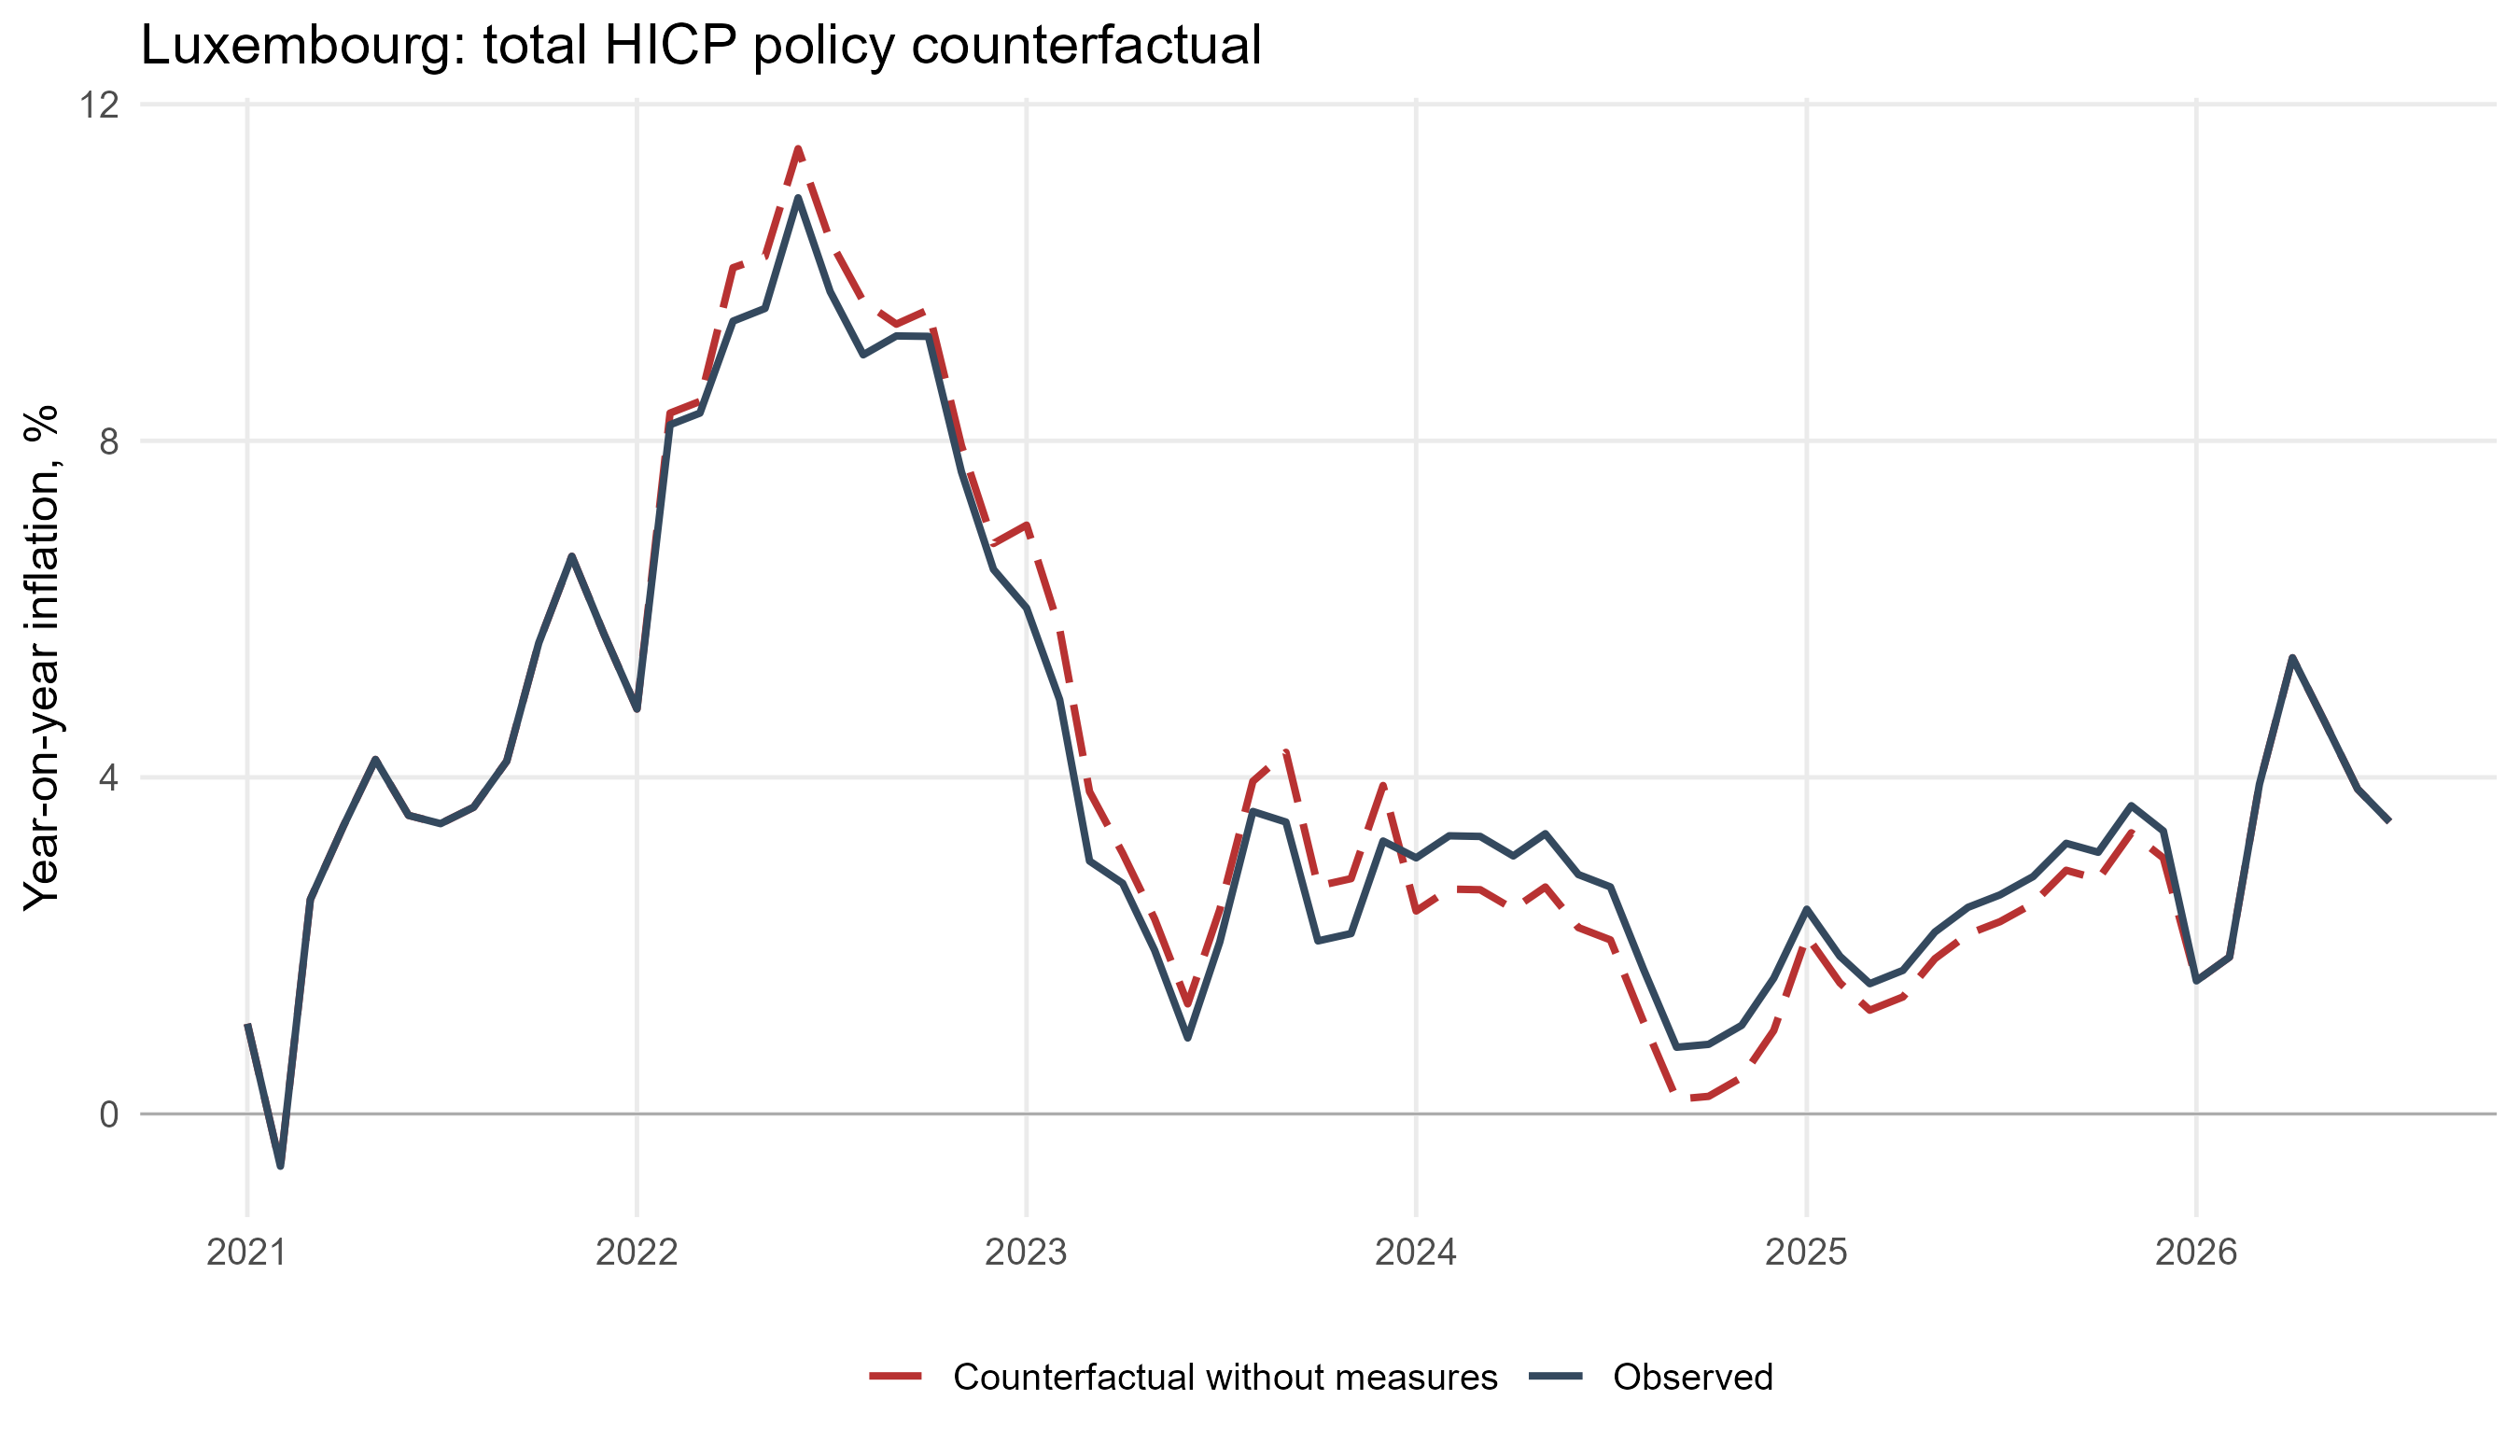
\includegraphics[width=\linewidth,height=0.225\textheight,keepaspectratio]{fig/policy_total_cpi_counterfactual_inflation_LU_luxembourg.png}\\[-0.4em]\textbf{(b) Luxembourg}
\end{minipage}

\vspace{0.25em}
\begin{minipage}[t]{0.485\textwidth}\centering
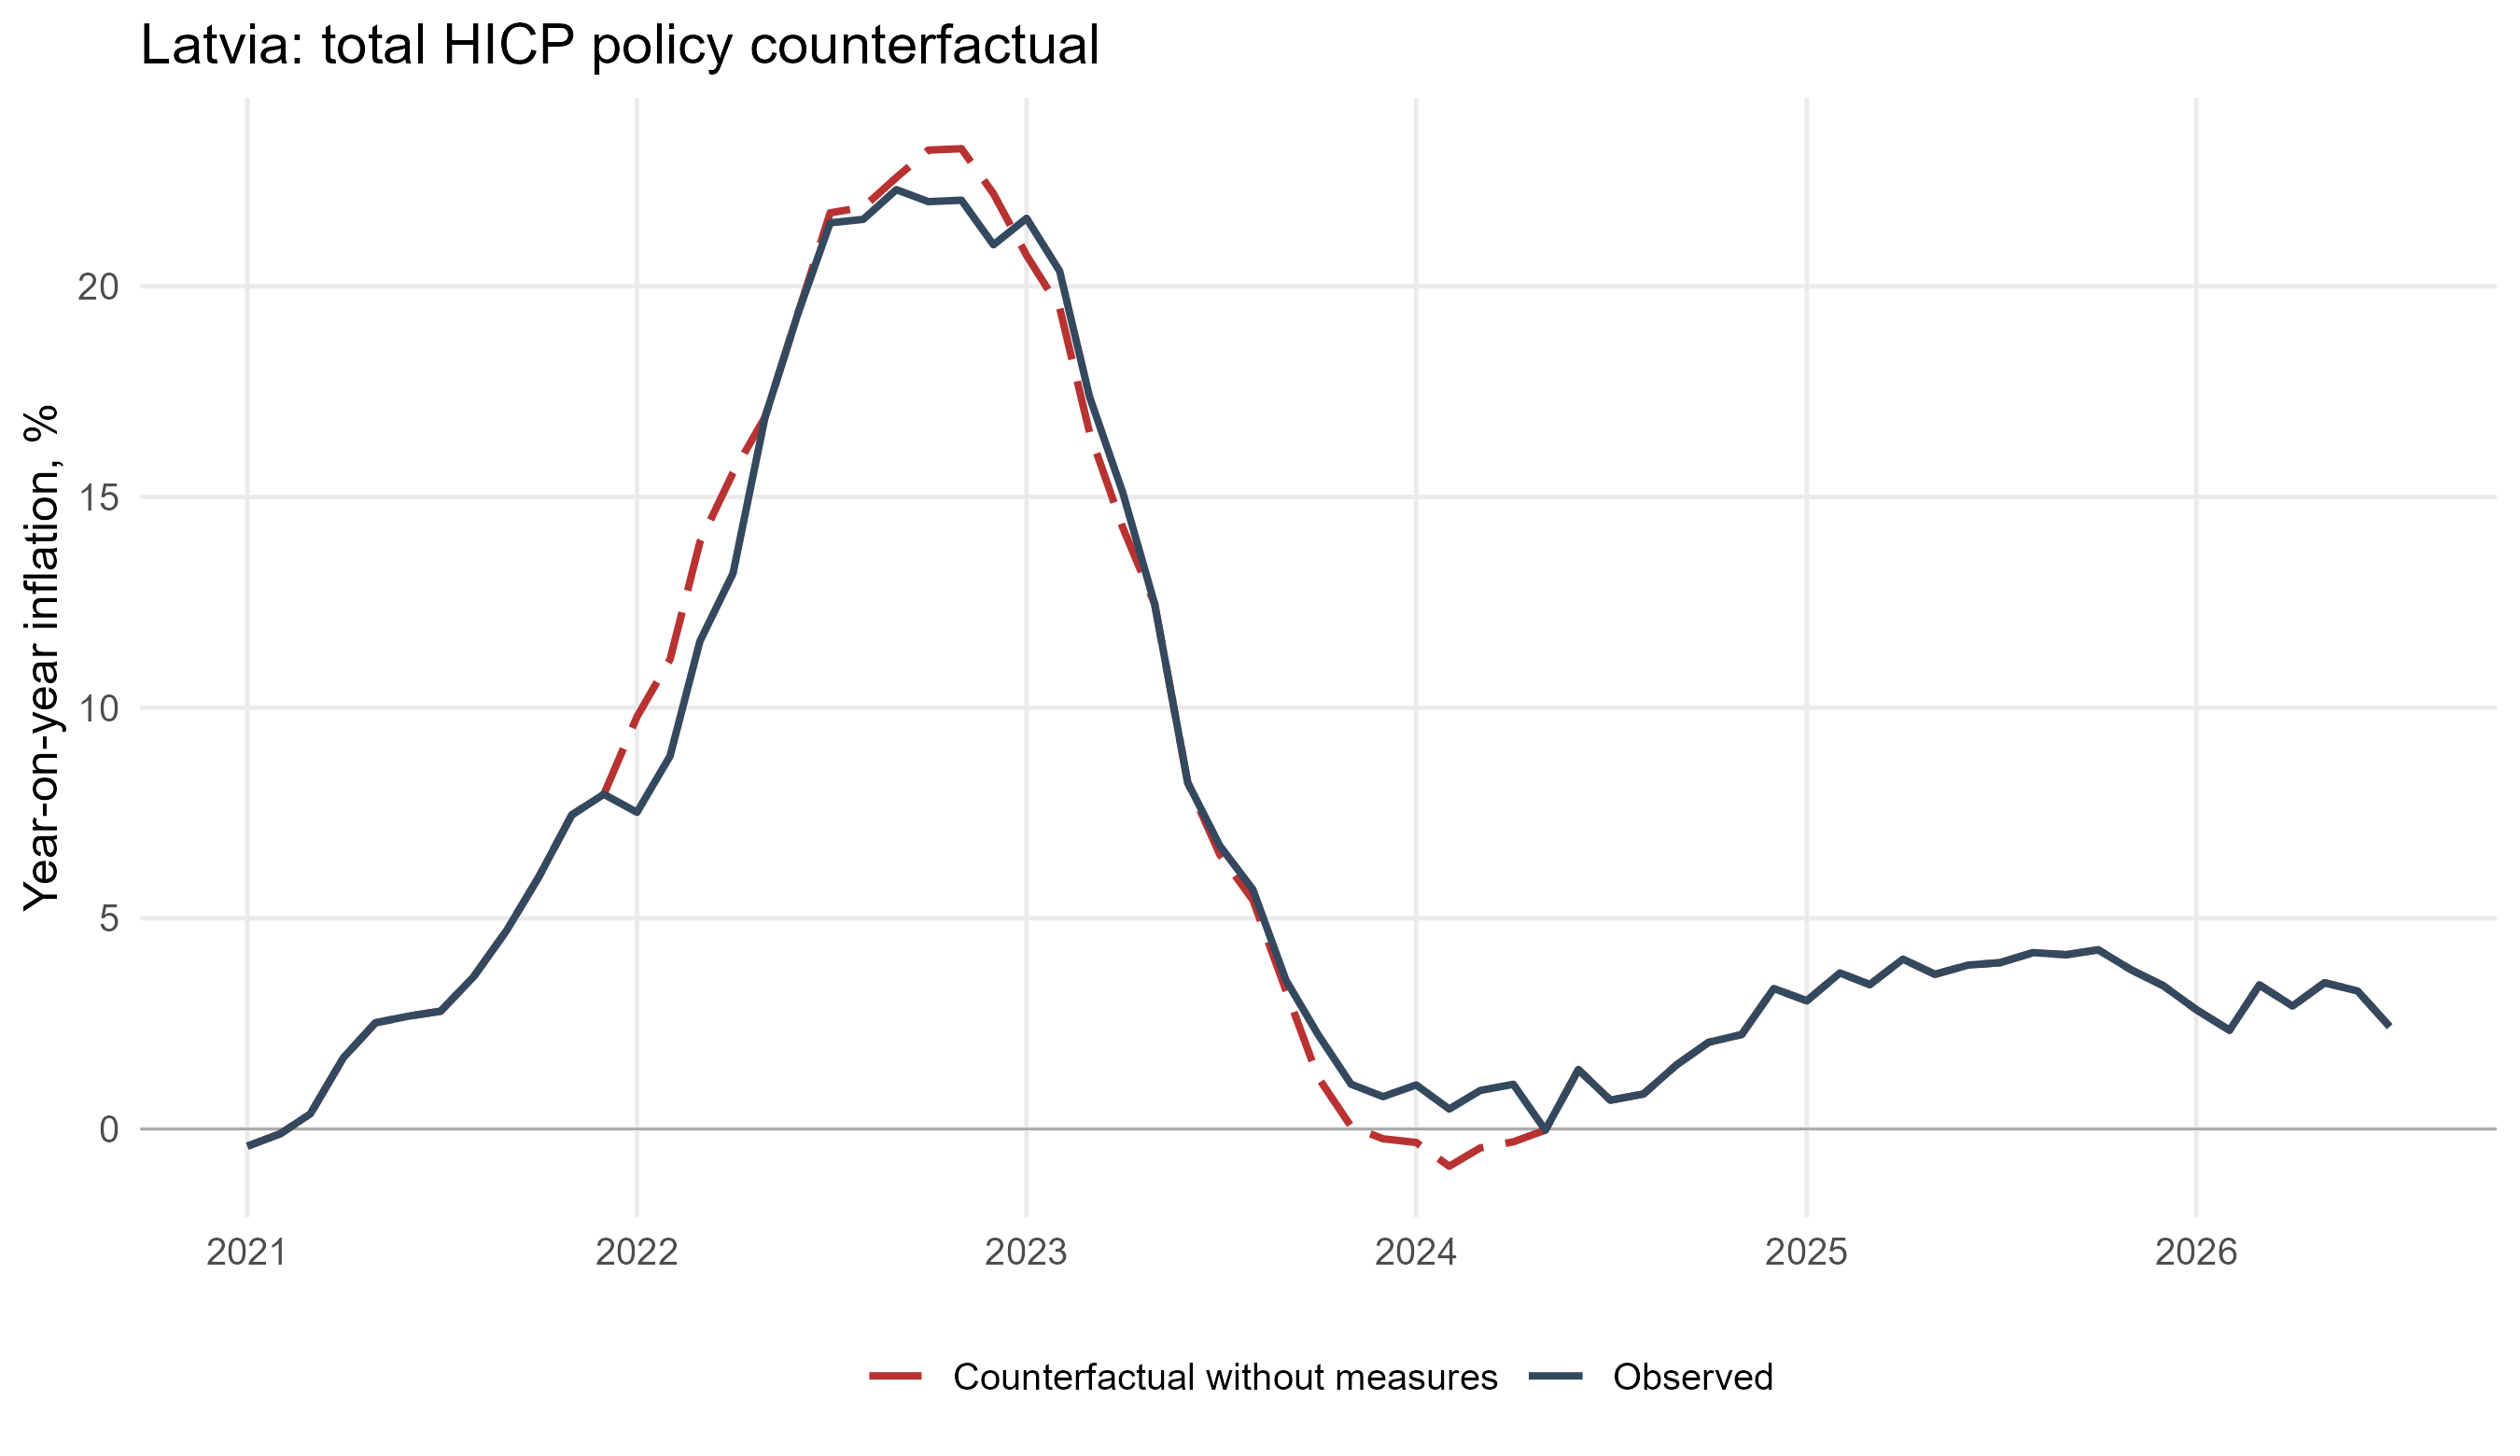
\includegraphics[width=\linewidth,height=0.225\textheight,keepaspectratio]{fig/policy_total_cpi_counterfactual_inflation_LV_latvia.png}\\[-0.4em]\textbf{(c) Latvia}
\end{minipage}\hfill
\begin{minipage}[t]{0.485\textwidth}\centering
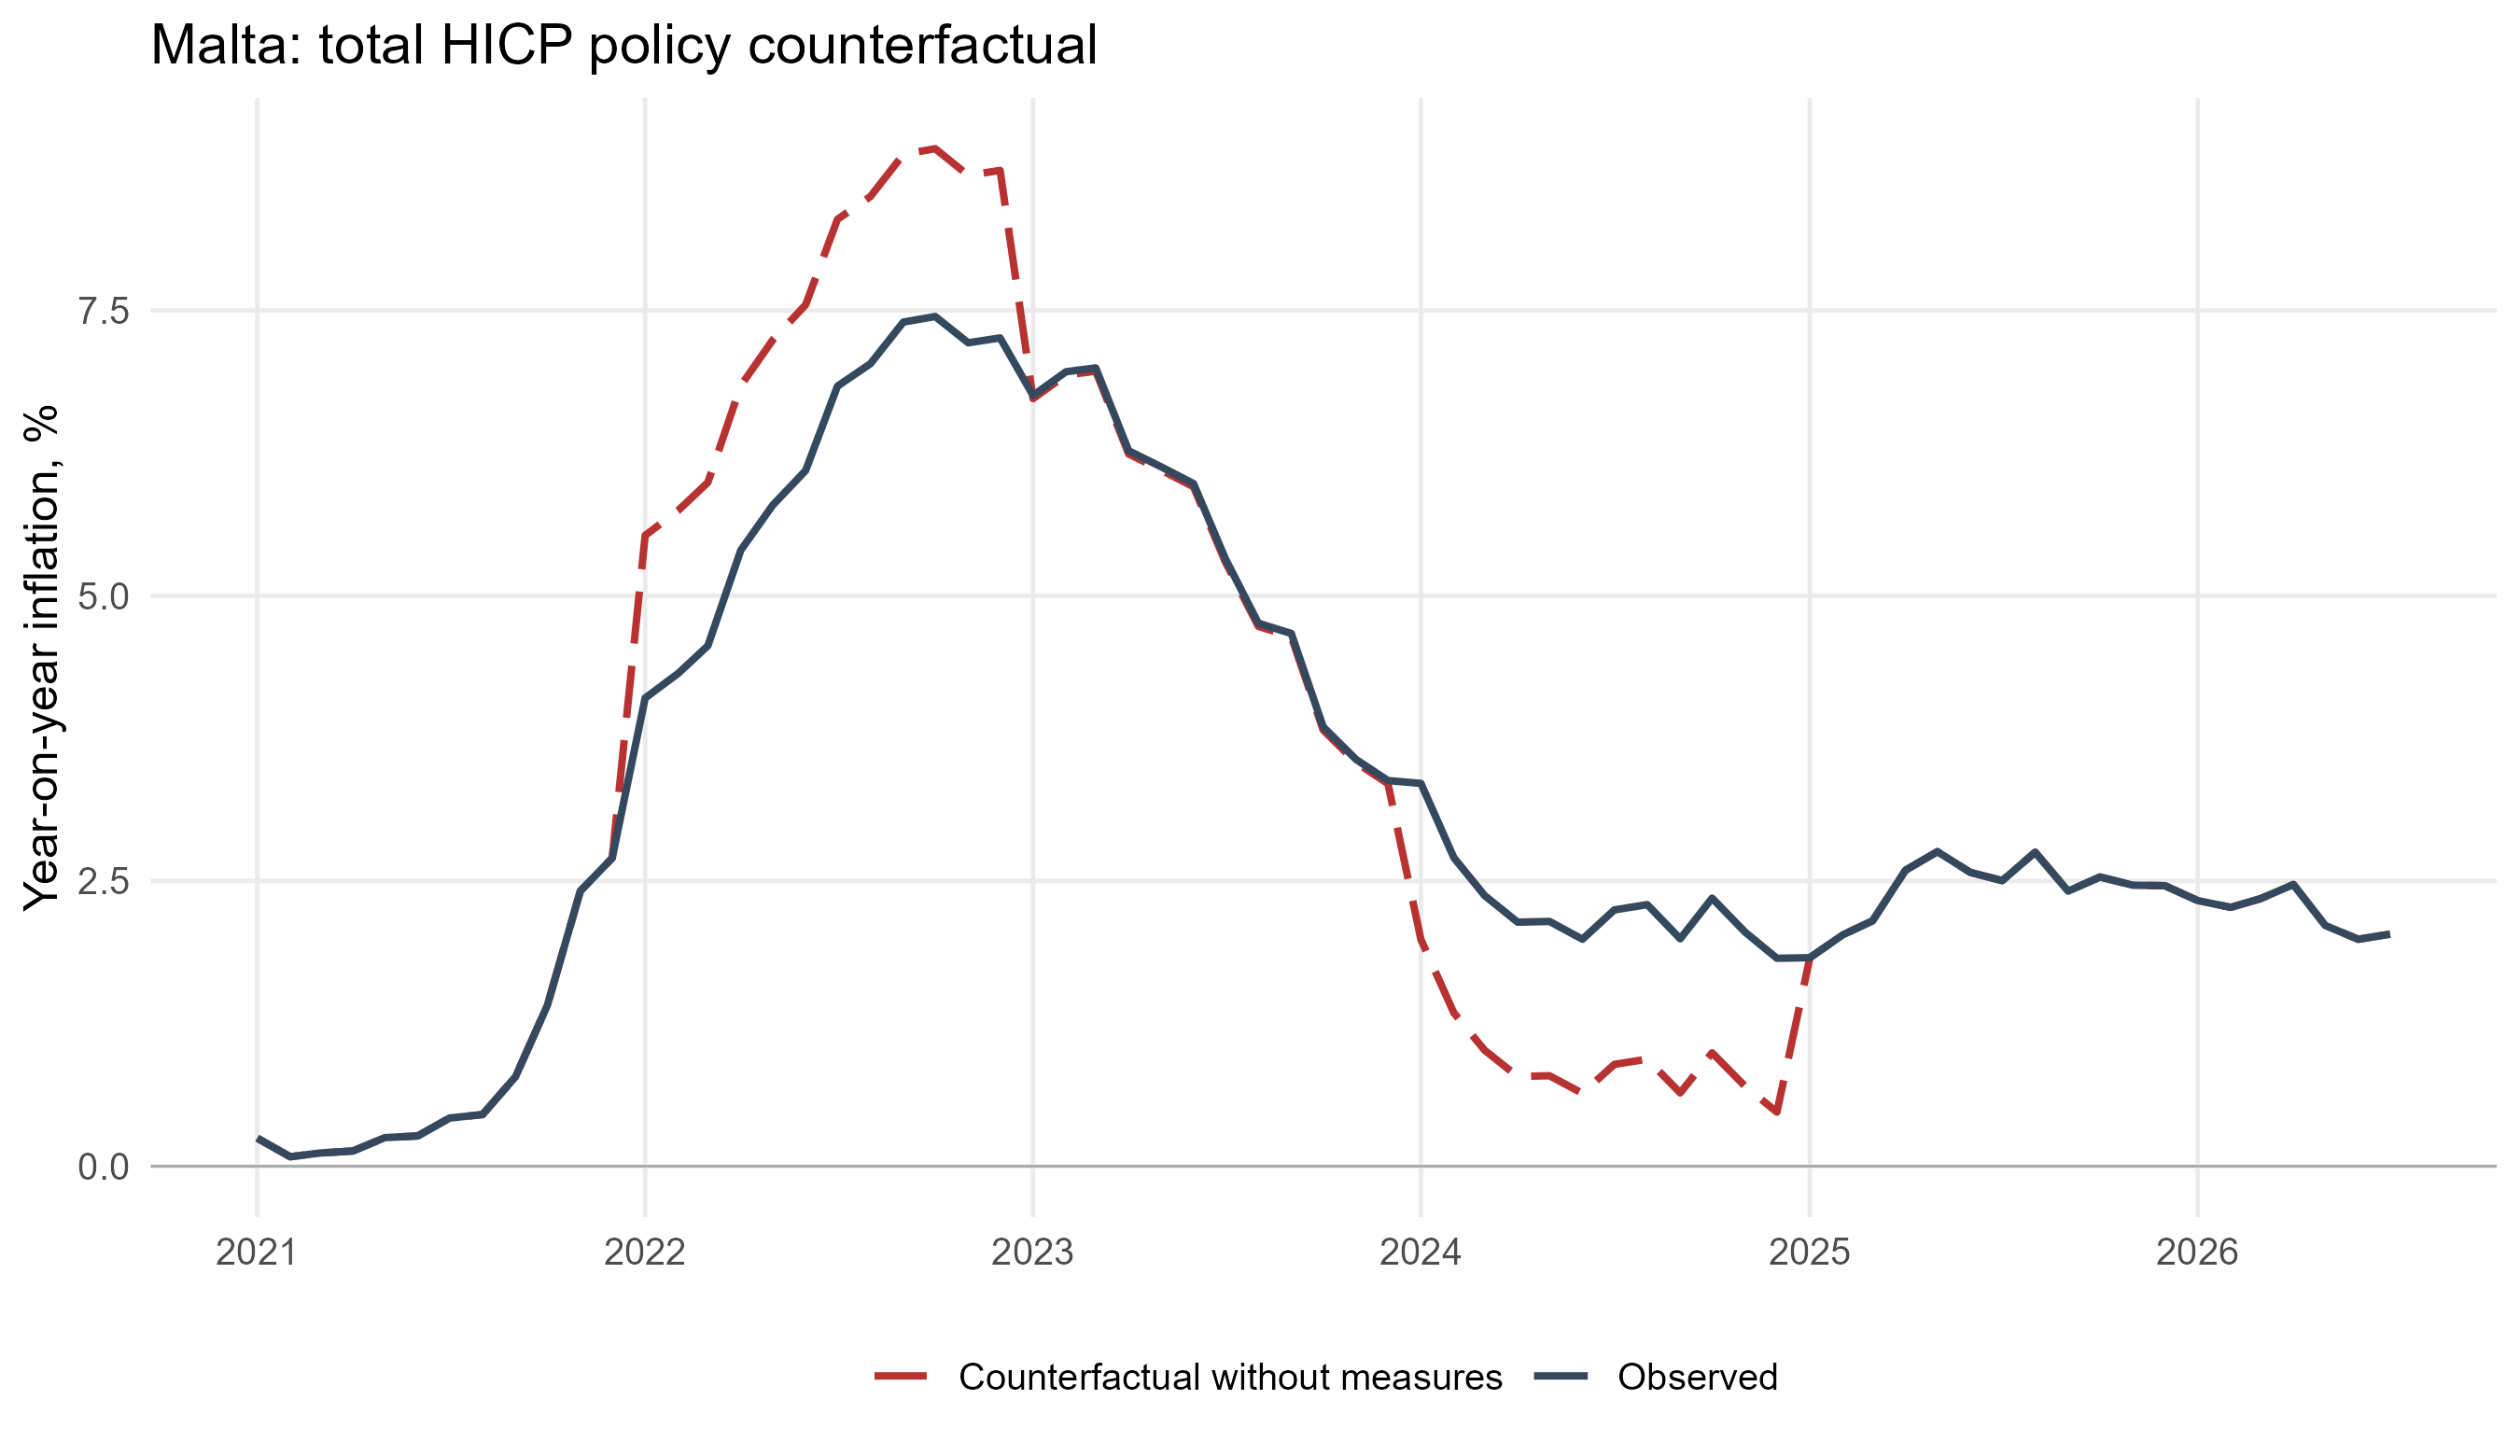
\includegraphics[width=\linewidth,height=0.225\textheight,keepaspectratio]{fig/policy_total_cpi_counterfactual_inflation_MT_malta.png}\\[-0.4em]\textbf{(d) Malta}
\end{minipage}

\vspace{0.25em}
\begin{minipage}[t]{0.485\textwidth}\centering
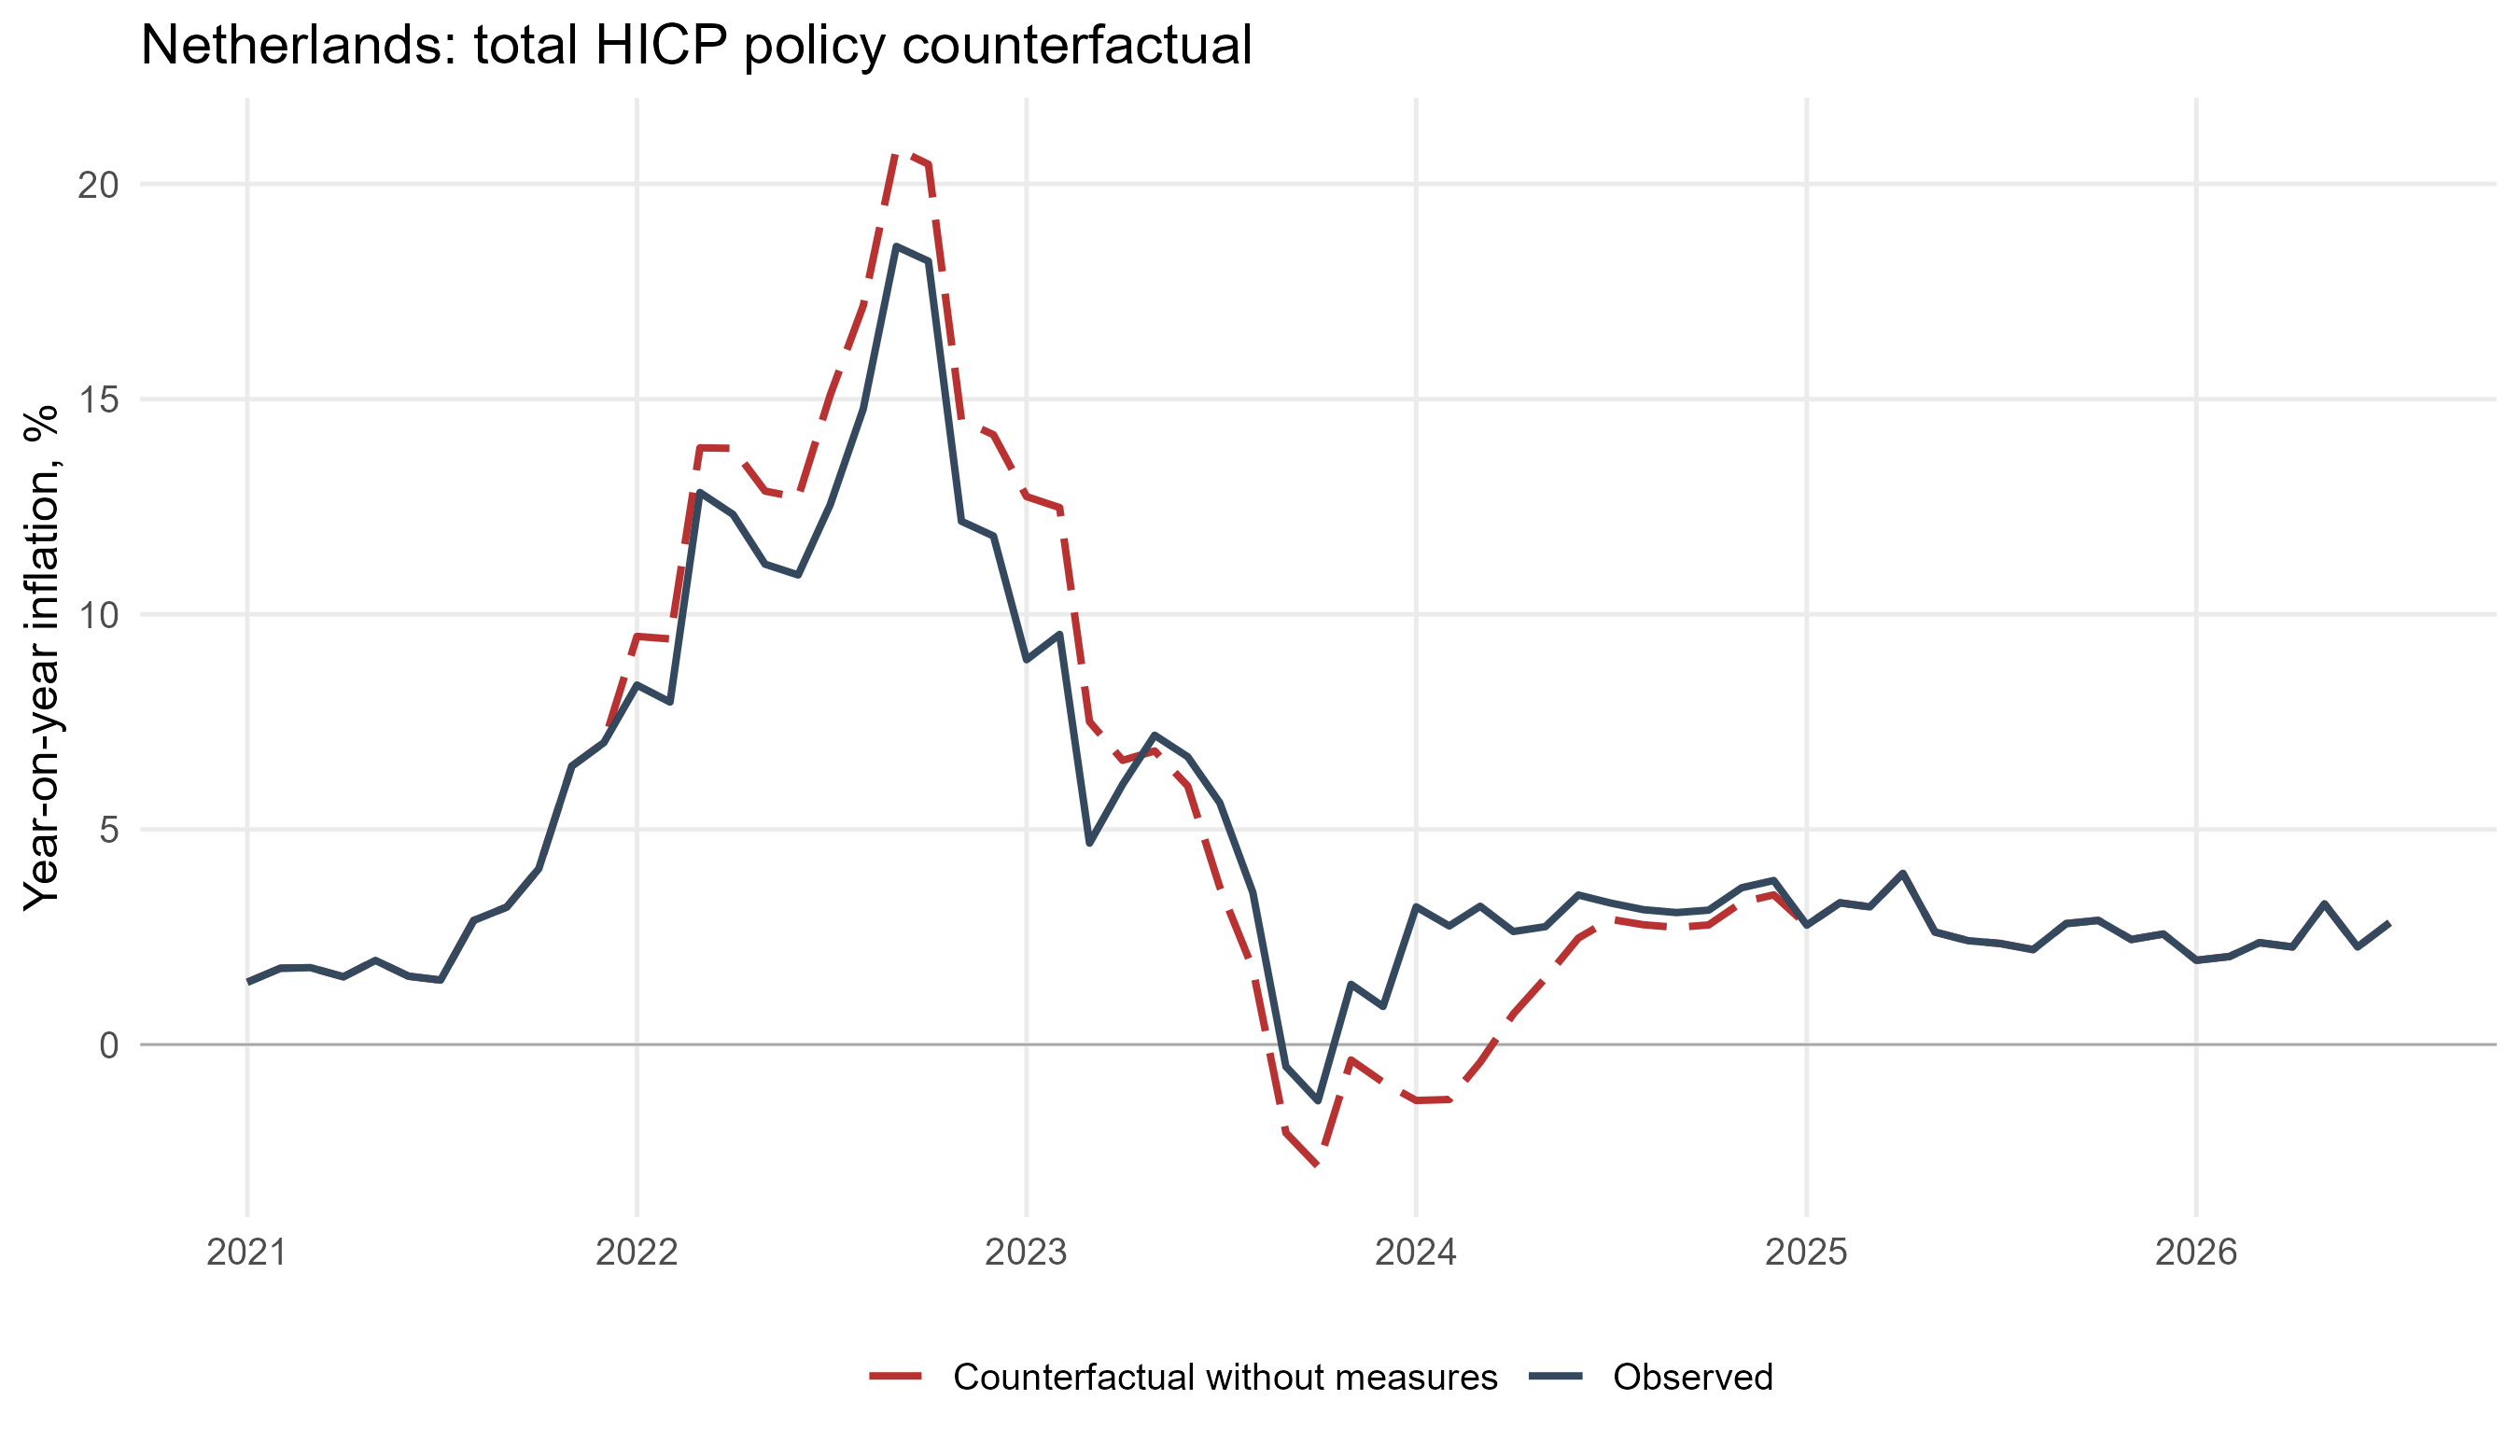
\includegraphics[width=\linewidth,height=0.225\textheight,keepaspectratio]{fig/policy_total_cpi_counterfactual_inflation_NL_netherlands.png}\\[-0.4em]\textbf{(e) Netherlands}
\end{minipage}\hfill
\begin{minipage}[t]{0.485\textwidth}\centering
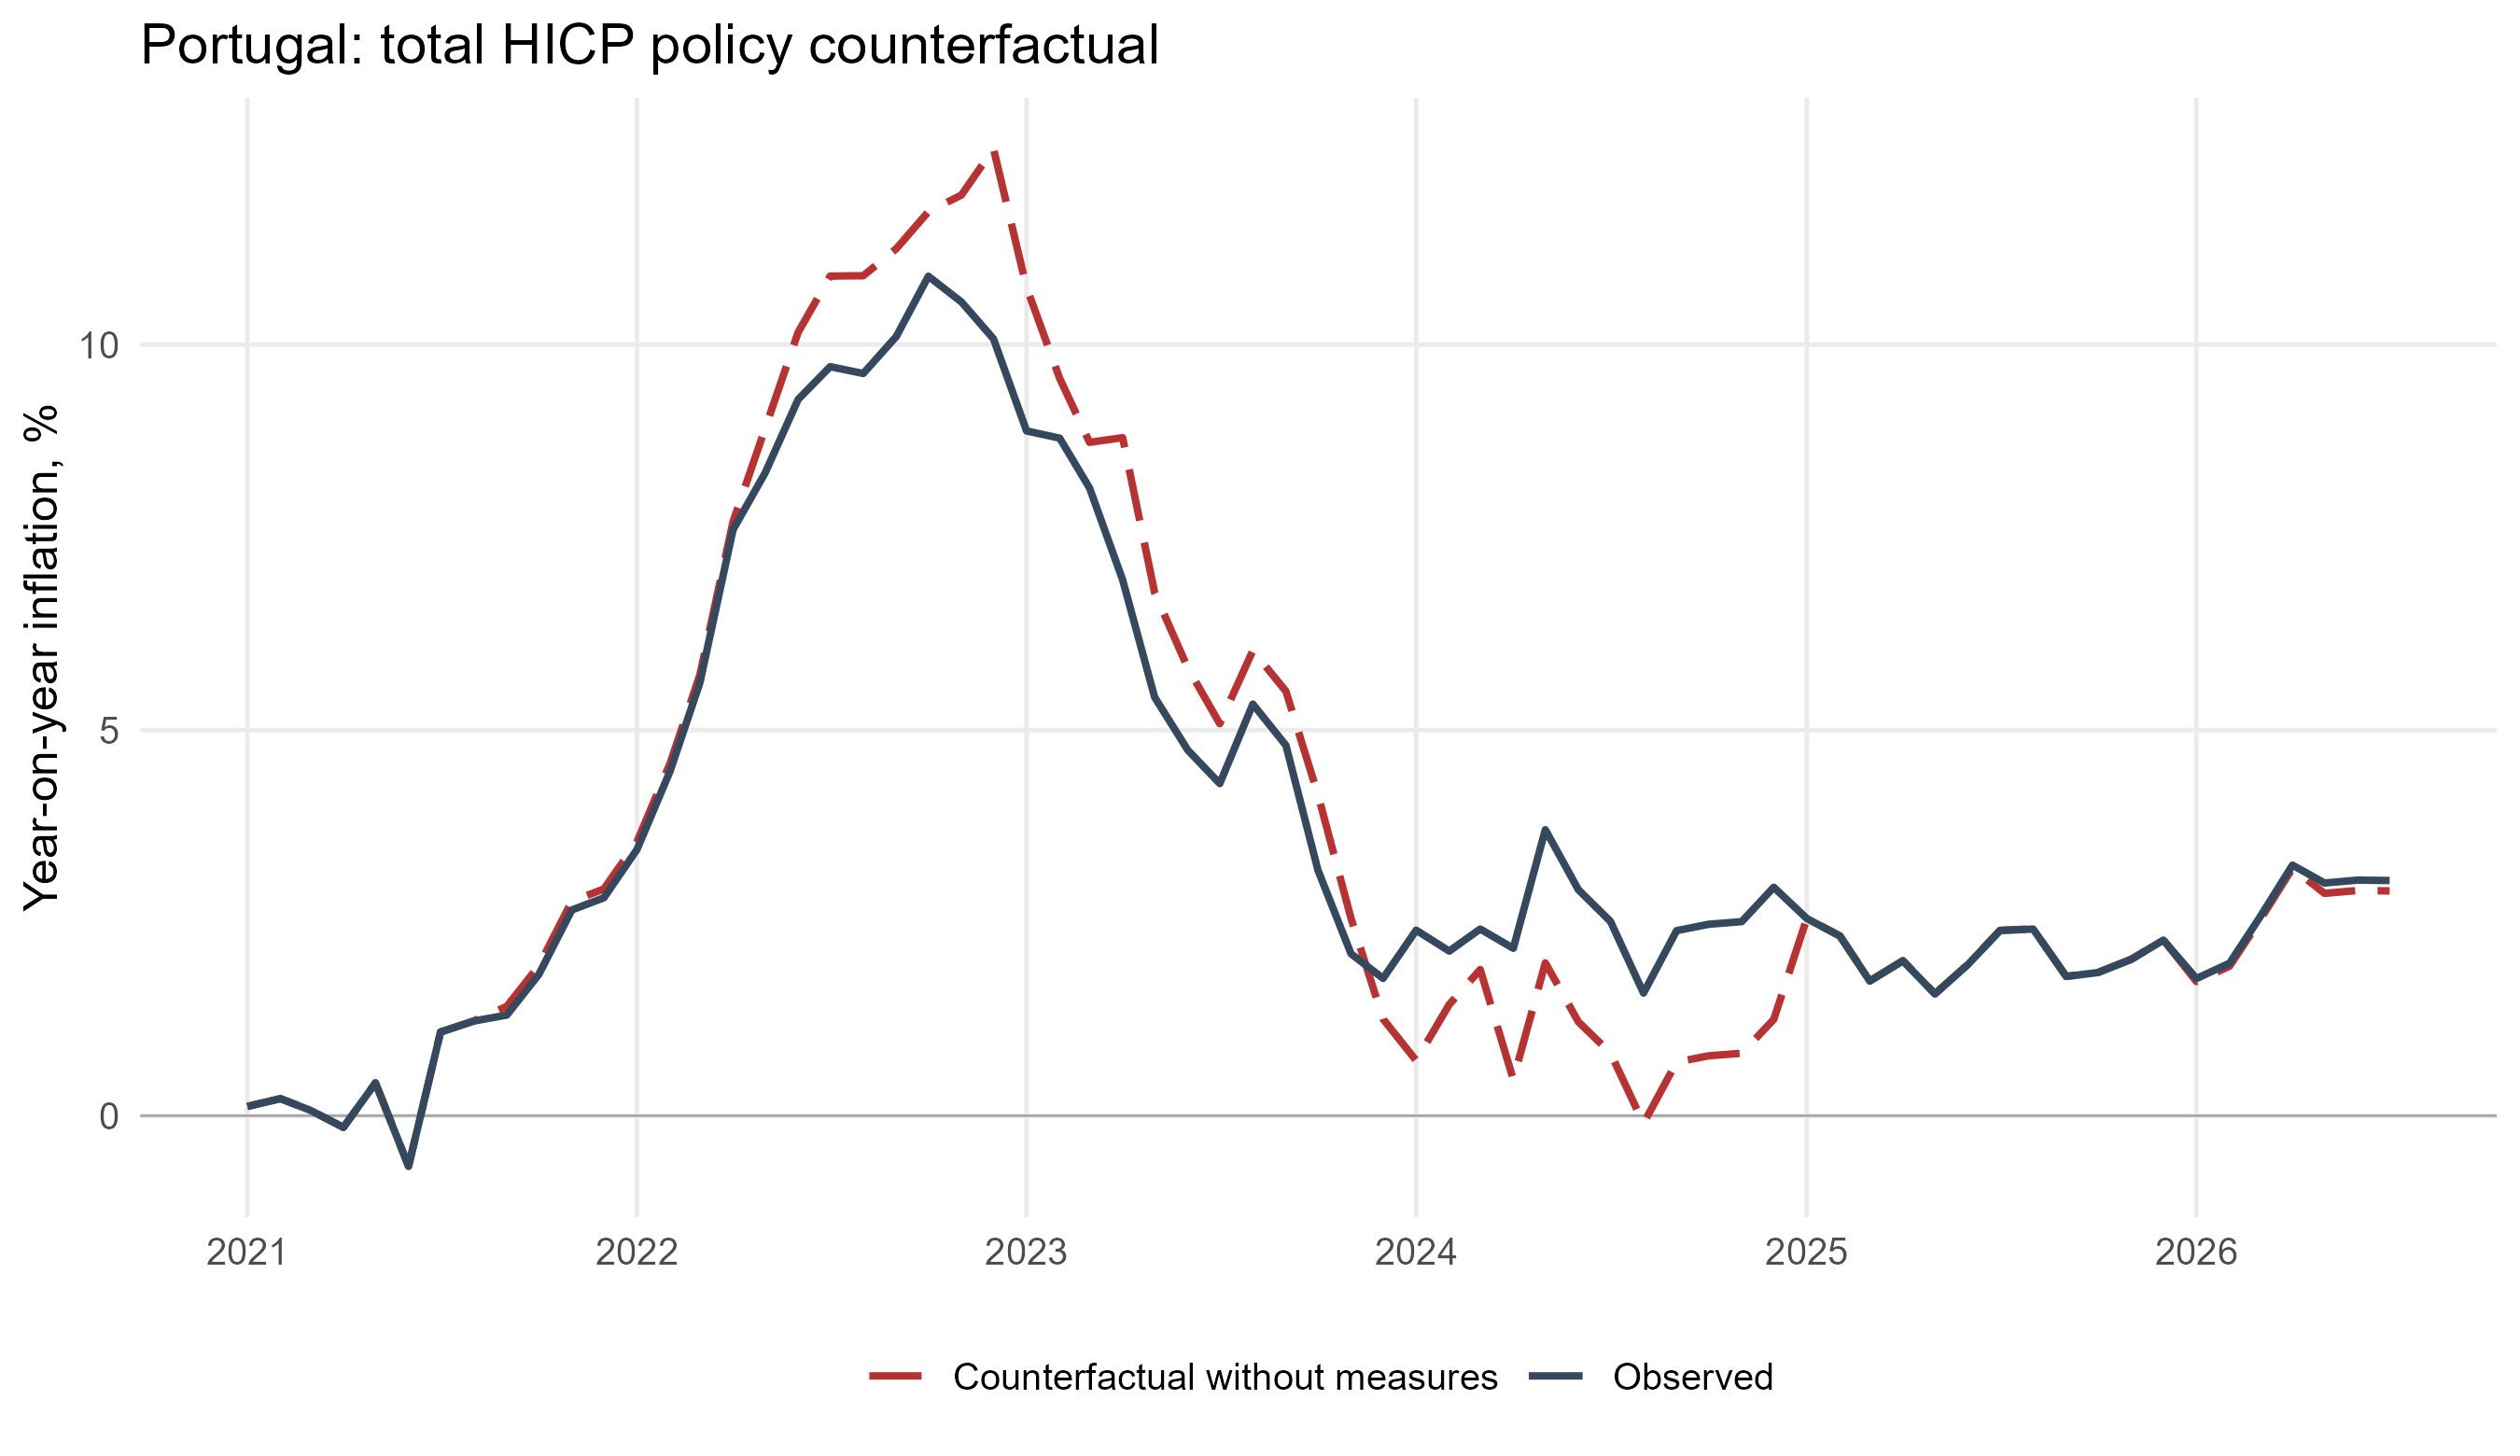
\includegraphics[width=\linewidth,height=0.225\textheight,keepaspectratio]{fig/policy_total_cpi_counterfactual_inflation_PT_portugal.png}\\[-0.4em]\textbf{(f) Portugal}
\end{minipage}
\caption{Observed and counterfactual inflation: Lithuania, Luxembourg, Latvia, Malta, Netherlands, Portugal}
\label{fig:country-counterfactuals-3}
\end{figure}
\clearpage

\begin{figure}[H]
\centering
\begin{minipage}[t]{0.485\textwidth}\centering
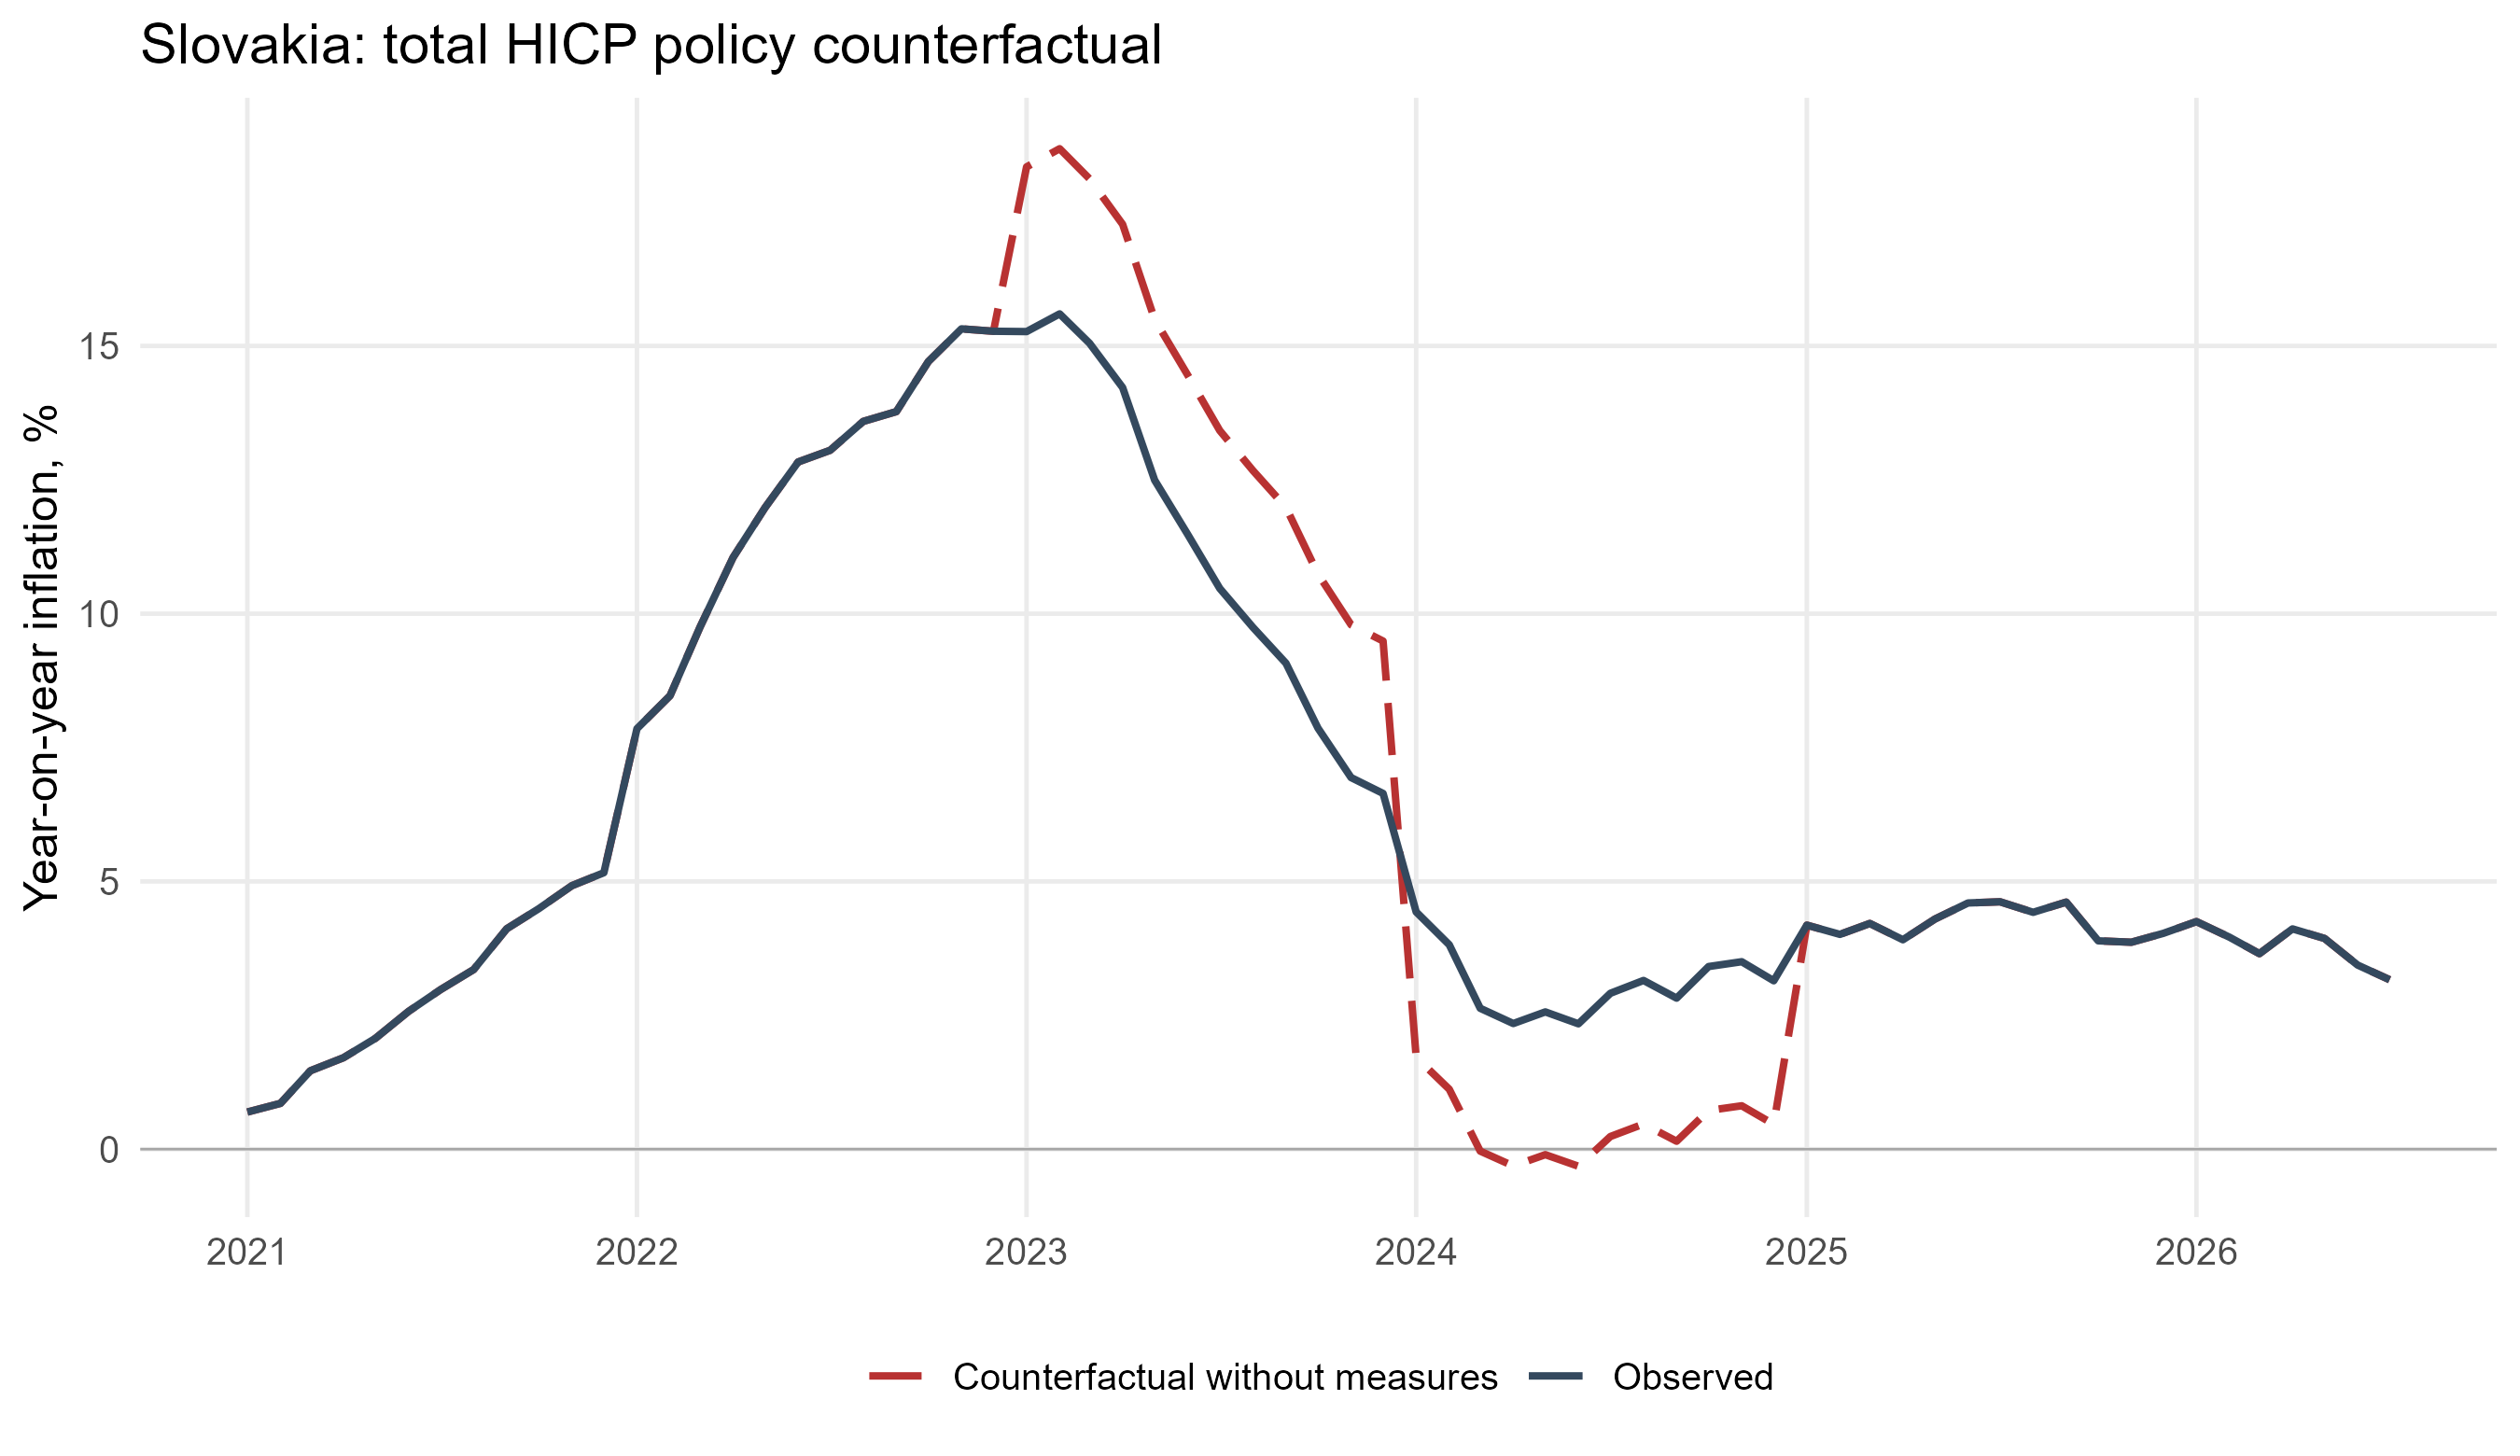
\includegraphics[width=\linewidth,height=0.225\textheight,keepaspectratio]{fig/policy_total_cpi_counterfactual_inflation_SK_slovakia.png}\\[-0.4em]\textbf{(a) Slovakia}
\end{minipage}\hfill
\begin{minipage}[t]{0.485\textwidth}\centering
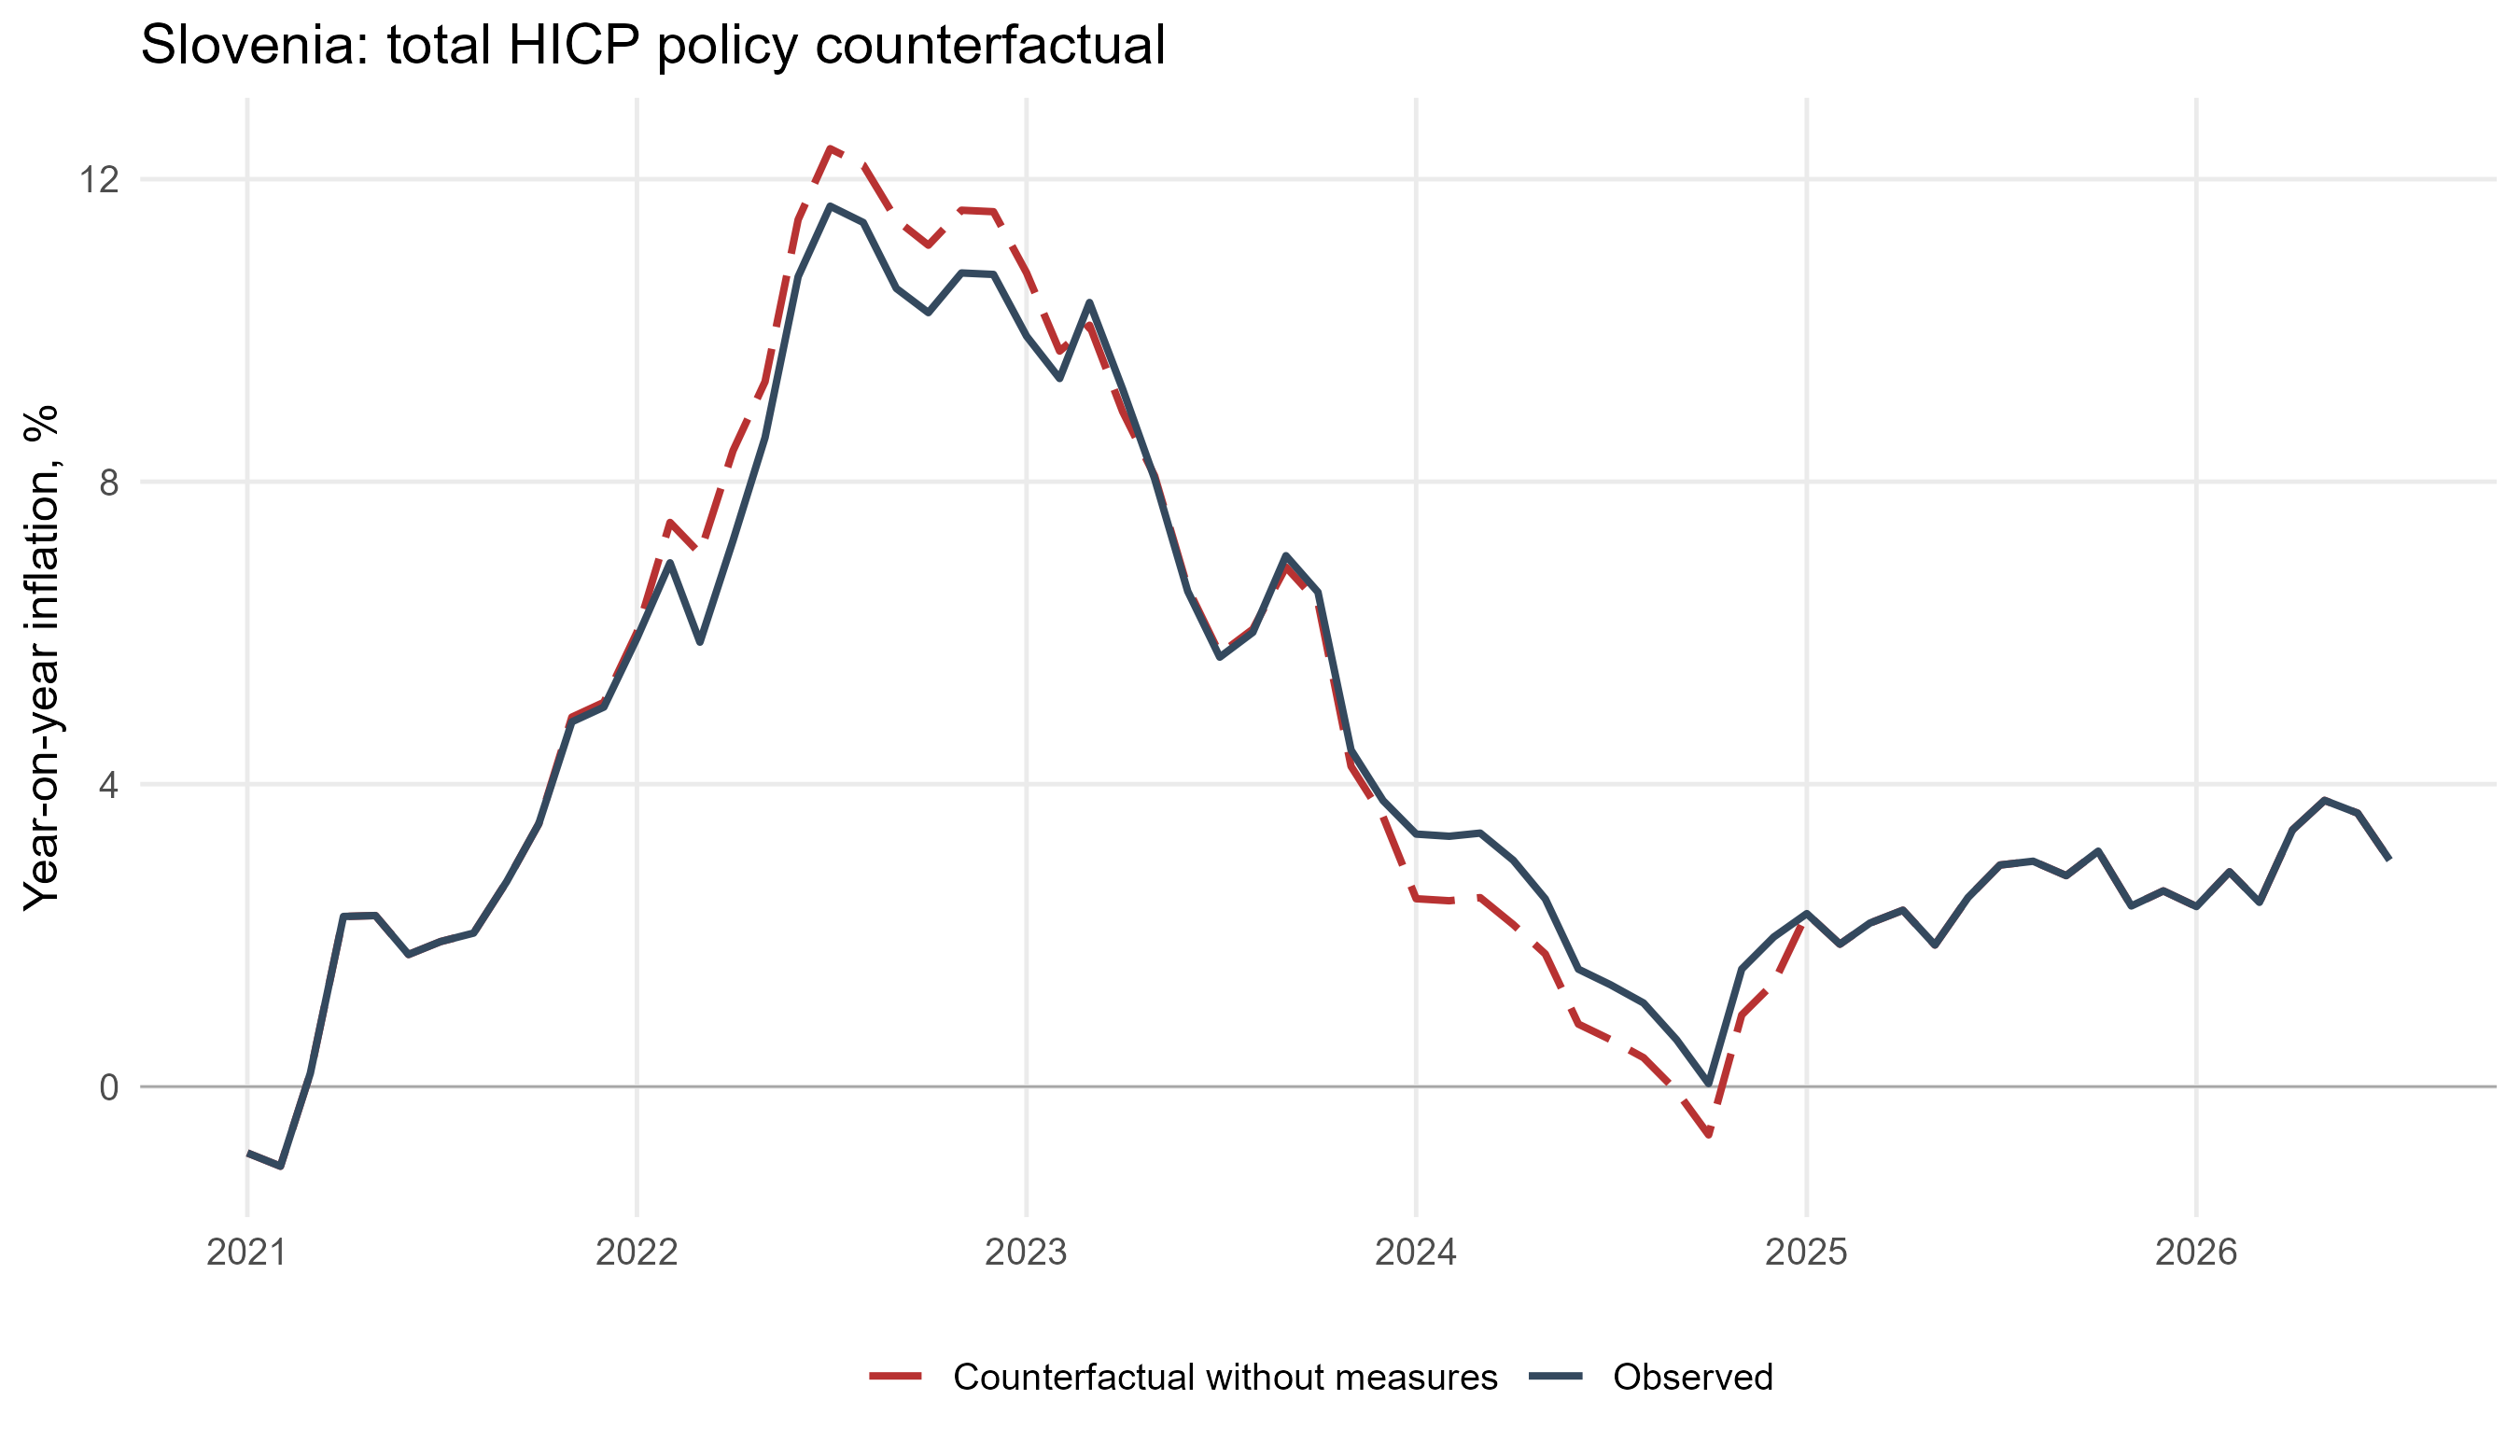
\includegraphics[width=\linewidth,height=0.225\textheight,keepaspectratio]{fig/policy_total_cpi_counterfactual_inflation_SI_slovenia.png}\\[-0.4em]\textbf{(b) Slovenia}
\end{minipage}
\caption{Observed and counterfactual inflation: Slovakia, Slovenia}
\label{fig:country-counterfactuals-4}
\end{figure}
\clearpage

\subsection{Product Decomposition of Policy Effects}
\label{sec:app-policy-product-differences}

Table~\ref{tab:ea20-counterfactual-income-gap-product-contributions} decomposes the aggregate effects by product group. Housing energy accounts for most of the reduction, while vehicle-operation expenditure partly offsets the fall in individual dispersion.

\begin{table}[H]
\small
\setlength{\tabcolsep}{8pt}

\caption{\label{tab:ea20-counterfactual-income-gap-product-contributions}Product-group contributions of household price policies to individual P20--P80 inflation dispersion and Q1--Q5 inflation inequality, 2021--2023}
\centering
\resizebox{\textwidth}{!}{%
\begin{tabular}[t]{l>{\centering\arraybackslash}p{1.45cm}*{6}{>{\centering\arraybackslash}p{1.25cm}}}
\toprule
Product group & \shortstack{Weight\\(2022, \%)} & \multicolumn{6}{c}{Inflation inequality}\\
\cmidrule(lr){3-8}
 &  & \multicolumn{3}{c}{Individual P20--P80} & \multicolumn{3}{c}{Income Q1--Q5}\\
\cmidrule(lr){3-5} \cmidrule(lr){6-8}
 &  & 2021 & 2022 & 2023 & 2021 & 2022 & 2023\\
\midrule
Food and non-alcoholic beverages & 17.8 & -0.2 & -0.3 & 0.3 & 0.0 & 0.0 & 0.0\\
Alcoholic beverages, tobacco and narcotics & 4.6 & 0.0 & 0.2 & -0.4 & 0.0 & 0.0 & 0.0\\
Clothing and footwear & 5.6 & -0.1 & -0.1 & 0.0 & 0.0 & 0.0 & 0.0\\
Housing maintenance and furnishings & 8.0 & 0.1 & 0.3 & 0.5 & 0.0 & 0.0 & 0.0\\
Water, electricity, gas and other fuels & 6.8 & -0.8 & -4.3 & -1.1 & -0.1 & -0.7 & -0.5\\
\addlinespace
Operation of personal transport equipment & 6.3 & 0.0 & 2.0 & -0.1 & 0.0 & 0.1 & 0.0\\
Transport (excluding vehicle operation) & 9.6 & 0.3 & -1.2 & -0.2 & 0.0 & 0.0 & 0.0\\
Other & 41.1 & 0.6 & 1.6 & 0.3 & 0.0 & 0.0 & 0.0\\
\midrule
\textbf{Total} & \textbf{100.0} & \textbf{-0.1} & \textbf{-1.8} & \textbf{-0.7} & \textbf{-0.1} & \textbf{-0.6} & \textbf{-0.6}\\
\bottomrule
\end{tabular}
}%
\vspace{-0.4em}
\begin{flushleft}
\footnotesize{Notes. Policy effects are observed minus counterfactual product contributions, in percentage points. The first block decomposes the effect on the P80 minus P20 range of annual household inflation, evaluating each scenario at its own national percentile households and averaging national contributions with annual HICP country weights over the 19-country household sample; Portugal is excluded. The second block decomposes the Q1 minus Q5 gap for all 20 euro-area countries. Annual rates compare annual-average indices. Product weights are 2022 EA20 expenditure shares. Sources: Eurostat, HBS 2020 microdata, national statistical institutes, authors' calculations.}
\end{flushleft}
\end{table}

\clearpage

